\chapter{Survey of Surveys (SoS)} 
\label{chap:SoS}
\bibentry{mcnabb2017sos} \cite{mcnabb2017sos} \\
\chapterquote{
But nowadays there's lots of other journals and it takes more and more effort to make sure that you know what's happening.}
{Jim Blinn, 1998}

\newpage
{\footnotesize \hypersetup{linkcolor=black}
\minitoc}
\newpage

% \begin{figure}
%   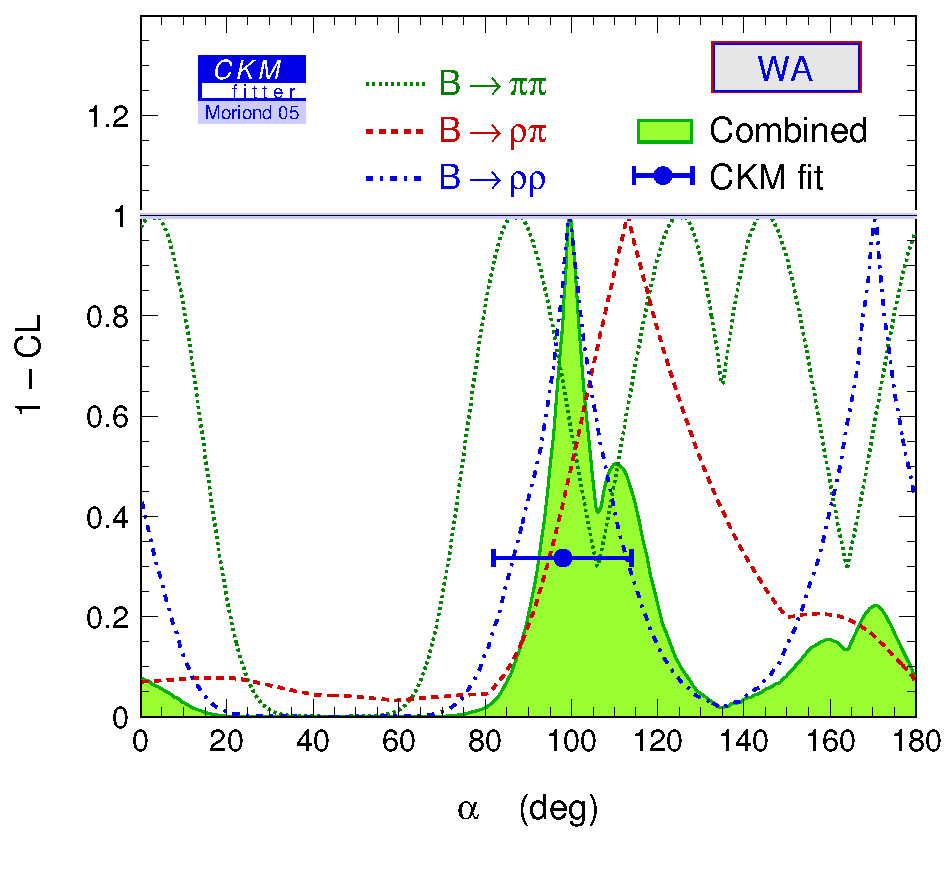
\includegraphics[width=\largefigwidth]{ckmfitter-alpha-combined}
%   \caption[CKM Fitter constraints on \alphaCKM.]%
%   {CKM Fitter constraints on \alphaCKM from combined \BToPiPi,
%     \BToRhoPi and \BToRhoRho decay analyses.}
%   \label{fig:CKMFitter}
% \end{figure}

\topskip0pt
\vspace*{4cm}
\section*{Chapter Abstract}
%\begin{abstract}
Information visualization as a field is growing rapidly in popularity since the first information visualization conference in 1995. However, as a consequence of its growth, it is increasingly difficult to follow the growing body of literature within the field. Survey papers and literature reviews are valuable tools for managing the great volume of previously published research papers, and the quantity of survey papers in visualization  has reached a critical mass.  To this end, this survey paper takes a quantum step forward by surveying and  classifying literature survey papers in order to help researchers understand the current landscape of Information Visualization. It is, to our knowledge, the first survey of survey papers (SoS) in Information Visualization. This paper classifies survey papers into natural topic clusters which enables readers to find relevant literature and develops the first classification of classifications. The paper also enables researchers to identify both mature and less developed research directions as well as identify future directions. It is a valuable resource for both newcomers and experienced researchers in and outside the field of Information Visualization and Visual Analytics.
%\end{abstract}
\newpage

%-------------------------------------------------------------------------
\section{Introduction and Motivation}
When we first reviewed potential survey papers, we looked at Smart City Visualization. After a small search, we found a book that fit our decided niche \cite{ciuccarelli2014depicting}. Due to this, we changed our views on writing a survey on car movement and found a paper by Chen et al.\ \cite{chen2015survey}. At this point, we tried two different avenues including geospatial and human movement, where we found papers for each \cite{nusrat2016state,gavrila1999visual}. At this point, we decided that a survey of surveys would be a good avenue forward. We looked at the benefits of surveying different survey papers which would allow us to gain a good understanding of unsolved problems found across the whole landscape, specifically for scale and zooming problems which we discuss throughout the paper.


\textit{"It used to be that SIGGRAPH was the only place that would publish computer graphics papers, and so all you had to do was read the SIGGRAPH Conference Proceedings and you knew you were up to date. But nowadays there's lots of other journals and it takes more and more effort to make sure that you know what's happening."} This quote is taken from Jim Blinn's renowned keynote speech at SIGGRAPH 98 \cite{blinn1998ten}. Decades later this theme is still considered one of the most important challenges for research in any field.

 Information Visualization is a rapidly evolving research field defined as "the communication of abstract data through the use of interactive visual interfaces" \cite{keim2006challenges}. Because of this, many researchers spend countless hours on research and development of Information Visualization techniques only to discover that research on a given topic has already been published. Survey papers and literature reviews are valuable and critical tools for managing the great number of previously published research papers. However even the number of survey papers themselves has reached a critical mass, thus inspiring a quantum step forward.

In this first undertaking of a survey of surveys (SoS), we aim to present the landscape of rapidly evolving research within Information Visualization. In order to emphasize open directions for future work, we present literature reviews of papers that survey research topics, and extract essential information from them systematically as a guide for both newcomers and experts in the field and beyond. We then classify over 80 survey papers to examine trends and themes that have recently been published. Our contributions to the field include:
\begin{itemize}
\item  A quantum step in literature review papers presenting the first meta-survey, i.e. a `Survey of Surveys' (SoS).
\item A novel classification of survey literature in the field of Information Visualization, which can be used as a guide for new researchers or a tool for field experts.
\item The first classification of literature classification schemes.
\item A structured overview of both mature and less developed future research directions that cover the domain of Information Visualization.
\end{itemize}

\begin{table}[t]
\ra{1.2}
\footnotesize
\centering
\rowcolors{1}{white}{black!05}
\begin{tabularx}{0.7\textwidth}{|X|c|}
\hline \rowcolor{black!15}
\textbf{Conferences \& Journals} & \textbf{Related Papers} \\ \hline
%\rowcolor{black!30}  &  Papers \\ 
The Annual EuroVis Conference & 20  \\
IEEE TVCG Journal & 18 \\
IEEE Pacific Visualization Symposium & 2 \\
IEEE VAST Conference & 3 \\
The Annual Eurographics Conference & 3 \\
Journal of Visual Languages \& Computing & 2 \\
Information Visualization Journal & 5 \\
Computer Graphics Forum & 3 \\
ACM Computing Surveys & 0 \\
Other & 30 \\ 
\hline
\rowcolor{black!15} \centering 
Total: & 86 \\
\hline
\end{tabularx}
\caption{A list of literature sources we search for survey papers, with the quantity of papers identified from each. For paper searching, we use IEEE Xplore  \cite{ieeexplore}, ACM Digital Library \cite{acmdigitallibrary}, Google Scholar \cite{scholar}, and Vispubdata \cite{isenberg2017VPD}} \label{table:searchTable}
\end{table}

\subsection{Literature-based Challenges in the Field}
There are at least three major difficult challenges within this field:
\begin{enumerate}
\item \textit{Understanding what has been already been done}: Many researchers end up losing time due to challenges associated with literature searches. As the Information Visualization landscape grows, so does the number of papers, conferences, and journals. This makes it increasingly difficult to find topic related papers. 
\item \textit{Understanding what areas in the domain have yet to be explored}: A researcher may not be truly sure whether a paper does not exist. This is a logical uncertainty. Until the point a paper is discovered, a researcher may still be unsure whether their development has been explored or not.
\item \textit{Making sure your discoveries are not ignored}: Papers are published to present discoveries in their field. However, due to the volume of published material, papers can be missed, forgotten, or reinvented. This challenge is also highlighted by Jim Blinn \cite{blinn1998ten}.
\end{enumerate}

The SoS aims to address these challenges by surveying a collection of over 80 survey papers to enable a quick overview of the scope of research directions, what has already been done, and which directions are more open for research. We provide systematic summaries of these survey papers for those with interest in the field. This serves as a valuable starting point for young researchers and a practical reference guide for field experts. We also believe this survey of surveys will reach audiences beyond the field of information visualization and visual analytics, and entice more researches towards the area.

\subsection{Literature Search Methodology}
Our survey search methodology includes a combination of linear-search and relation-search. Our starting point includes reviewing previous EuroVis State-of-the-Art (STAR) papers. The linear search focuses on looking at each journal or conference and checking each paper that includes keywords such as 'Survey', 'Taxonomy', or 'State-of-the-Art'. The relation-search includes searching the references of each survey paper for related survey papers. 

Sources that are searched within our SoS following this methodology are summarized in Table \ref{table:searchTable}. Our survey paper search lasted over a year.


\subsection{Classification Overview}
In order to classify each survey, we develop categorical dimensions. The dimensions are derived from previously published and well-known literature based on: 
\begin{enumerate}
\item An adapted Information Visualization pipeline model originally presented by Card et al.\ \cite{card1999readings}. A visual aid to this pipeline can be found in Figure \ref{fig: originalPipeline}.
\item Subject-based clusters guided by SurVis \cite{beck2016visual} and the survey paper topics themselves.
\end{enumerate}
Both of these dimensions are explained in greater detail in Sections \ref{sec:infovispip} and \ref{sec:subbasedclusters}.
\subsubsection{The Information Visualization Pipeline} \label{sec:infovispip}
The Information Visualization pipeline model we use to classify the surveys is based on that presented by Card et al.\ in their classic book \textit{'Readings in Information Visualization'} \cite{card1999readings} (See Figure \ref{fig: originalPipeline}). The pipeline describes the transition of raw data into a visualization which is visible to a user. This consists of (1) raw data transformed into data tables via the use of data transformations. (2) Data tables transformed into visual structures via the use of visual mappings. (3) Visual structures transformed into views via the use of view transformations. The final step is (4) User input manipulating the data in order to feed back into the pipeline.
\begin{figure}
\begin{center}
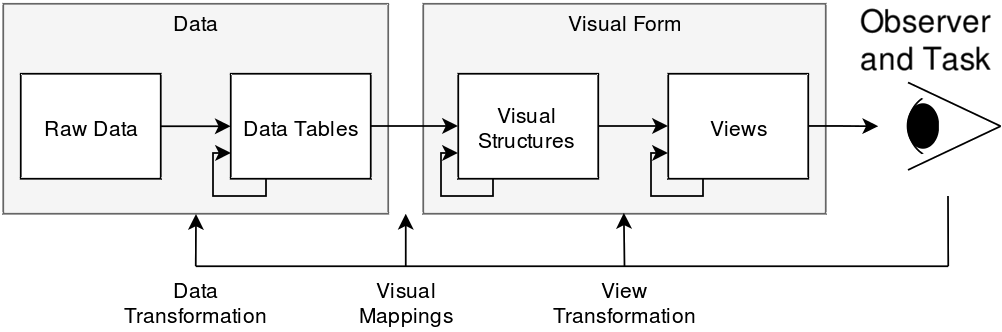
\includegraphics[width=0.9\textwidth]{images/customPipeline}
\caption{The original Information Visualization Pipeline model created by Card et al. \cite{card1999readings} which we adapt to design our modified classification.} \label{fig: originalPipeline}
\end{center}
\end{figure}
For the purpose of the SoS, the pipeline is adapted in order to facilitate the categorization process.
The following pipeline stages are used.
\begin{enumerate}

\item \textbf{Data Enhancement \& Transformation} - Data Enhancement and Transformation is used to describe the raw data that is transformed or enhanced in order to derive a data structure(s) that can be used for visualization. The classification also includes how the data is captured and how the data is classified. Survey papers that are data-centric are placed in this category. \label{class1}

\item \textbf{Visual Mapping \& Structure} - Visual Mapping and Structure defines the techniques to visualise data or data structures. This section also examines how a visualization is structured, such as how the mapping is used or the facets that are included. This category involves mapping the enhanced data to visual primitives, for example, color, opacity, textures, and geometry such as points, edges, as well as 2D and 3D shapes. Survey papers with an emphasis on visual mapping and structure are categorized here. \label{class2}

\item \textbf{Exploration and Rendering} - The three common types of view transformation are location probes that use location to reveal additional information, viewpoint controls which are used to scale or translate a view, and distortions which modify the visual structure \cite{card1999readings}. Exploration and Rendering looks at these transformations along with the rendered representation views and projections. This is the presented state a visualization takes upon completion and aims to present the data to the user. Survey papers with a focus on rendering and exploration are classified here. \label{class3}

\item \textbf{Interactive Analysis} - Analysis refers to how the user provides feedback to a visualization. A user can connect with a visualization manually, by modifying or transforming a view state, or by reviewing the use, effectiveness, and their knowledge on the visualization. This also includes selection protocols and mapping techniques such as task taxonomy or other viariations of selection. Survey papers with a focus on interactive analysis or tasks are placed here. \label{class4}

\item \textbf{Perception} - Perception examines the cognitive interperatation of a visualization from the perspective of a user. Perception can be viewed through the design and creation of user studies or papers relating the visual system to Information Visualization. Survey papers emphasizing perception and user-studies are placed in this category. \label{class5}

\end{enumerate}
These components form the basis of the first dimension of our classification. Figure \ref{fig: yearbreakdown} provides a breakdown of these classification by year.

\begin{figure*}
\begin{center}
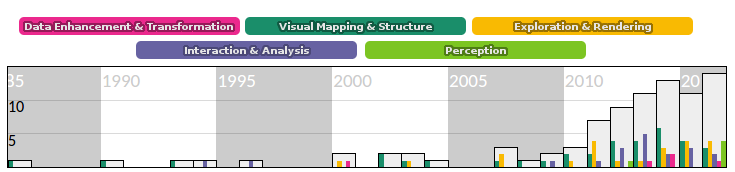
\includegraphics[width=1\textwidth]{images/yearbreakdownv2}
\caption{A histogram providing the frequency of surveys found for each year mapped along the x-axis. each bar represents one year whilst the y-axis provides the amount of survey papers found for each year that meet our scope (Section \ref{sec:scope}). The colored bars represent a further breakdown of the survey papers based on their given classification dimension (discussed in Section \ref{sec:infovispip}). The visualization is taken from the SoS literature browser \cite{surVis}.} \label{fig: yearbreakdown}
\end{center}
\end{figure*}

\subsubsection{Subject-based Clusters} \label{sec:subbasedclusters}
Literature and subject-based clusters group similarly focused survey papers. SurVis \cite{beck2016visual} is used as an aid in order to discover and diagnose suitable clusters, exploring keywords related to each paper. Survey papers that cite previous survey papers create natural topic clusters that are taken into account within our subject-based clusters. The subject clusters %for paper topics are found in Table \ref{table:clusters}.
are as follows --
\begin{table}[h!]
\scriptsize
\ra{1.42}
\centering
\begin{tabular}{|m{2cm}|p{3.5cm}|}
\hline
\multirow{2}{2cm}{\raggedright \textbullet ~Data-Centric} & $\diamond$ ~Data-Types\\ \cline{2-2}
& $\diamond$ ~Text-Focus\\ \hline \hline
\multirow{5}{2cm}{\raggedright \textbullet ~Multivariate \& Hierarchical} &$\diamond$ ~Hierarchical\\  \cline{2-2}
&$\diamond$ ~High-Dimensional \\&~~~~Overview\\ \cline{2-2}
&$\diamond$ ~Parallel Coordinates\\ \cline{2-2}
&$\diamond$ ~Glyphs\\ \hline \hline
\multirow{2}{2cm}{\raggedright \textbullet ~Graphs \& Networks} &$\diamond$ ~Graphs\\ \cline{2-2}
&$\diamond$ ~Networks\\ \hline \hline
\multirow{2}{2cm}{\raggedright \textbullet ~Geospace + Time} &$\diamond$ ~Temporal\\ \cline{2-2}
&$\diamond$ ~Geospatial\\ \hline \hline
\multicolumn{2}{|l|}{\textbullet ~~Coordinated Multiple Views}\\ \hline \hline
\multirow{6}{2cm}{\raggedright \textbullet ~Real-World \& ~~~~~Applications} &$\diamond$ ~Finance\\ \cline{2-2}
&$\diamond$ ~Healthcare\\ \cline{2-2}
&$\diamond$ ~Security\\ \cline{2-2}
&$\diamond$ ~Systems\\ \cline{2-2}
&$\diamond$ ~SoftVis\\ \cline{2-2}
&$\diamond$ ~Frameworks\\ \hline \hline
\multirow{3}{2cm}{\raggedright \textbullet ~~Overview} & $\diamond$~Focus+Context\\ \cline{2-2}
 & $\diamond$~Provenance\\ \cline{2-2}
& $\diamond$~General\\ \hline
\end{tabular}
\caption{Hierarchy of subject-based clusters.}
 \label{table:clusters}
\vspace{-0.6cm}
\end{table}
Data-Centric contains literature that focus on types of data, or data itself. Multivariate \& Hierarchical focus on structured data, or data that visualizes many dimensions. Graphs and Networks focus on literature that discusses nodes and edges used in visualization, usually standard 2D views. Geospace+Time review surveys with that look at dimensional data.  Coordinated Multiple Views (CMVs) centers around literature that examines the coordination or linkage between multiples. Real-World and Applications focuses on literature that reviews topics with an emphasis on practical data or with real-world users. Overview contains literature that provide a more broad survey of the information visualization landscape. A full breakdown of the topics can be found in Table \ref{table:clusters}.

%Clusters diagnosed:
%\begin{footnotesize}
%\begin{itemize}
%\item Data-Centric \vspace{-0.2cm}
%\begin{itemize}
%\item Data-Types
%\item Text-Focus \vspace{-0.2cm}
%\end{itemize}
%\item Multivariate \& Hierarchical \vspace{-0.2cm}
%\begin{itemize}
%\item Hierarchical
%\item High-Dimensional Overview
%\item Parallel Coordinates
%\item Glyphs \vspace{-0.2cm}
%\end{itemize}
%\item Graphs \& Networks \vspace{-0.2cm}
%\begin{itemize}
%\item Graphs
%\item Networks \vspace{-0.2cm}
%\end{itemize}
%\item Geospace+Time \vspace{-0.2cm}
%\begin{itemize}
%\item Temporal
%\item Geospatial \vspace{-0.2cm}
%\end{itemize}
%\item Coordinated Multiple Views (CMVs)
%\item Real-World \& Application \vspace{-0.2cm}
%\begin{itemize}
%\item Finance
%\item Healthcare
%\item Security
%\item Systems
%\item SoftVis
%\item Frameworks \vspace{-0.2cm}
%\end{itemize}
%\item Overview \vspace{-0.2cm}
%\begin{itemize}
%\item Focus+Context
%\item Provenance
%\item General
%\end{itemize} 
%\end{itemize}
%\end{footnotesize}

\subsection{SoS Scope} \label{sec:scope}
Restrictions are used in order to define, manage, and constrain the scope of the SoS. 

Firstly, only survey papers with a focus on Information Visualization and Visual Analytics found within the field are included. This means Scientific Visualization does not fall within the scope. There are several recent scientific visualization surveys not included. For purposes of this survey, we define scientific visualization (SciVis) as the following:

"Data that describes a physical phenomenon is defined as scientific data. Examples of this are fluid flow, living organisms, and data from the natural world."  For the purpose of this survey, Euclidean space-time coordinate data is considered Scientific Visualization. Lipsa et al.\ survey visualization in physical sciences, this does not meet the criteria of our survey \cite{lipsa2012visualization}. Edmunds et al.\ present a framework for flow visualization \cite{edmunds2012surface}. Flow visualization is considered SciVis. Blascheck et al.\ 's survey on Eye-Tracking data is a review of literature focused on data from a physical phenomenon and can therefore be classed as SciVis\cite{blascheck2014state}.

Papers that focus on Computer Vision are not considered within scope. Datondji et al.\ present a survey focused on vision based traffic monitoring of road intersections. This is considered a computer vision topic and therefore does not meet the scope of the paper \cite{datondji2016survey}.

Computer graphics and Graph theory literature surveys are not considered in the scope of the SoS. Ghosh and Goswami present a paper reviewing unsolved problems in visibility graphs \cite{ghosh2013unsolved}. Although the paper works on graphs, the review focuses on the mathematics of graph theory and not visualization. Biomedical and computational biology are beyond the scope of this SoS. They are covered in an affiliated SoS called the SoS-MDV \cite{alharbi2017molecular}. 

Secondly, publication date is considered. This enables a clear emphasis on recent advancements, and what can be done at this time to increase our advancement in the field of Information Visualization. This is important as it allows us to provide a clearer message about future research fields, as the older survey papers may discuss research areas that are now mature. The emphasis for the SoS is between the years 2010 and 2016. As prior papers are still important, we include surveys that fall out of this time-frame onto our classification table, however, we do not include a detailed description of them. Older surveys that are included in the table only can shed historical light on where authors chose to publish visualization paper before the visualization community developed (prior to 1990).

Finally, the SoS emphasizes literature reviews, as opposed to comparison-oriented papers. Shneiderman et al.\ look at the innovation trajectories of treemaps, conemaps, and hyperbolic trees, but focus on the global state of each techniques' citations and papers, rather than a comparison of individual papers \cite{schneiderman2012innovation}. Sedlmair et al.\ look at scatter-plot and dimension reduction technique choices, as well as multiple reduction techniques for scatter-plots. These techniques are compared as abstractions\cite{sedlmair2013empirical}. Papers such as these are not given a detailed summary, however, we include these in the classification table for completeness.




\begin{table*}[p]
\tiny
\centering
\newcommand{\multitext}[1]{\multirow{2}{*}[1.5ex]{\rotcell{#1}}}
\ra{1}
\begin{tabularx}{1\textwidth}{|m{1.3cm}|r|C|C|C|C|C|}
\hhline{~~|-----|}
\multicolumn{2}{c|}{~}&\multicolumn{5}{c|}{\textbf{\fillCellTitle Information Visualization Pipeline}}\\
\hhline{~~|-----|}
\rowcolor{black!02} \multicolumn{2}{c|}{\cellcolor{white}} & Data Enhancement \& Transformation & Visual Mapping \& Structure & Exploration \& Rendering & Interaction \& Analysis & Perception \\  \hline
%-------------------------------------------------------------------------------------------------------%
\fillCellTitle &
\fillCellSubHeader Data-Types&
&
\colorbox{lime}{\cite{sedlmair2012taxonomy}} \colorbox{yellow}{\cite{sedlmair2013empirical}} \colorbox{lime}{\cite{zhou2015survey}}&
\colorbox{pink}{\cite{de2003visual}} \colorbox{lime}{\cite{isaacs2014state}} &
&
\\ \hhline{|>{\arrayrulecolor{black!15}}->{\arrayrulecolor{black}}|------|}

%-------------------------------------------------------------------------------------------------------%
\multirow{-4}{1.3cm}{\centering \fillCellTitle \textbf{Data-Centric}} & \fillCellSubHeader Text-Focus &
\colorbox{lime}{\cite{wanner2014state}} &
\colorbox{yellow}{\cite{silic2010visualization}} \colorbox{yellow}{\cite{nualart2014we}} \colorbox{yellow}{\cite{gan2014document}} \colorbox{lime}{\cite{janicke2015on}} \colorbox{yellow}{\cite{janicke2016visual}} &
\colorbox{lime}{\cite{kucher2015text}} &
\colorbox{yellow}{\cite{alencar2012seeing}}  \colorbox{lime}{\cite{federico2016survey}}&
\\ \hline
%-------------------------------------------------------------------------------------------------------%
\fillCellTitle &
\fillCellSubHeader Hierarchical &
\colorbox{lime}{\cite{alsallakh2014visualising}}&
\colorbox{lime}{\cite{elmqvist2010hierarchical}} \colorbox{lime}{\cite{schulz2011design}} \colorbox{yellow}{\cite{schneiderman2012innovation}}&
&
&
\\ \hhline{|>{\arrayrulecolor{black!15}}->{\arrayrulecolor{black}}|------|}
%-------------------------------------------------------------------------------------------------------%

\fillCellTitle&
\fillCellSubHeader High-Dimensional Overview&
&
&
\colorbox{lime}{\cite{bertini2011quality}} \colorbox{lime}{\cite{liu2015visualising}} &
\colorbox{pink}{\cite{buja1996interactive}} &
\\ \hhline{|>{\arrayrulecolor{black!15}}->{\arrayrulecolor{black}}|------|}
%-------------------------------------------------------------------------------------------------------%
\fillCellTitle &
\fillCellTitle\fillCellSubHeader Parallel Coordinates &
&
\colorbox{lime}{\cite{heinrich2013state}} &
&
\colorbox{yellow}{\cite{dasgupta2012conceptualizing}} &
\colorbox{lime}{\cite{johansson2016evaluation}} \\ \hhline{|>{\arrayrulecolor{black!15}}->{\arrayrulecolor{black}}|------|}
%-------------------------------------------------------------------------------------------------------%
\multirow{-7}{1.3cm}{\centering \fillCellTitle \textbf{Multivariate \& Hierarchical}} &
\fillCellSubHeader Glyphs &
&
\colorbox{pink}{\cite{ward2002taxonomy}} \colorbox{lime}{\cite{borgo2013glyph}} &
&
&
\colorbox{lime}{\cite{fuchs2016systematic}} \\ \hline
%-------------------------------------------------------------------------------------------------------%
\fillCellTitle &
\fillCellSubHeader Graphs &
\colorbox{yellow}{\cite{kobourov2004force}} &
\colorbox{lime}{\cite{von2011visual}} \colorbox{lime}{\cite{beck2014state}} \colorbox{lime}{\cite{kerracher2014design}} \colorbox{lime}{\cite{vehlow2015state}} &
\colorbox{pink}{\cite{herman2000graph}} \colorbox{yellow}{\cite{zhou2013edge}}&
\colorbox{yellow}{\cite{archambault2013map}} \colorbox{lime}{\cite{kerracher2015task}} \colorbox{lime}{\cite{kerracher2015visual}}&
\\ \hhline{|>{\arrayrulecolor{black!15}}->{\arrayrulecolor{black}}|------|}
%-------------------------------------------------------------------------------------------------------%
\multirow{-5}{1.3cm}{\centering \fillCellTitle \textbf{Graphs \& Networks}} &
\fillCellSubHeader Networks &
&
\colorbox{yellow}{\cite{zaidi2014analysis}}&
\colorbox{lime}{\cite{behrisch2016matrix}} &
\colorbox{lime}{\cite{ahn2014task}}&
\\ \hline
%-------------------------------------------------------------------------------------------------------%

\fillCellTitle &
\fillCellSubHeader Temporal &
&
\colorbox{lime}{\cite{cottam2012watch}}   &
\colorbox{lime}{\cite{bach2014review}} &
 &
\\ \hhline{|>{\arrayrulecolor{black!15}}->{\arrayrulecolor{black}}|------|}
%-------------------------------------------------------------------------------------------------------%
\multirow{-2}{1.3cm}{\centering \fillCellTitle \textbf{Geospace + Time}}&
\fillCellSubHeader Geospatial &
&
\colorbox{pink}{\cite{tobler2004thirty}} \colorbox{pink}{\cite{dodge2008towards}} \colorbox{lime}{\cite{nusrat2016state}} &
\colorbox{lime}{\cite{chen2015survey}} &
\colorbox{lime}{\cite{nusrat2015task}}&
\\ \hhline{|+->{\arrayrulecolor{black}}|------|}
%-------------------------------------------------------------------------------------------------------%
\multicolumn{2}{|c|}{\fillCellTitle \textbf{Coordinated Multiple Views (CMVs)}}&
&
\colorbox{lime}{\cite{javed2012exploring}}  \colorbox{lime}{\cite{hadlak2015survey}} &
\colorbox{pink}{\cite{roberts2007state}} \colorbox{yellow}{\cite{gleicher2011visual}}&
&
\\ \hline
%-------------------------------------------------------------------------------------------------------%
\fillCellTitle &
\fillCellSubHeader Finance &
\colorbox{lime}{\cite{ko2016survey}} &
&
\colorbox{yellow}{\cite{flood2016application}}&
&
\\ \hhline{|>{\arrayrulecolor{black!15}}->{\arrayrulecolor{black}}|------|}
%-------------------------------------------------------------------------------------------------------%
\fillCellTitle &
\fillCellSubHeader Healthcare &
&
\colorbox{pink}{\cite{kosara2002visualization}} \colorbox{yellow}{\cite{west2015innovative}}&
\colorbox{yellow}{\cite{rind2011interactive}} &
&
\\ \hhline{|>{\arrayrulecolor{black!15}}->{\arrayrulecolor{black}}|------|}
%-------------------------------------------------------------------------------------------------------%
\fillCellTitle &
\fillCellSubHeader Security &
&
&
\colorbox{lime}{\cite{shiravi2012survey}} \colorbox{lime}{\cite{wagner2015survey}}  &
&
 \\ \hhline{|>{\arrayrulecolor{black!15}}->{\arrayrulecolor{black}}|------|}
%-------------------------------------------------------------------------------------------------------%
\fillCellTitle &
\fillCellSubHeader Systems &
&
\colorbox{yellow}{\cite{grammel2013survey}}&
&
\colorbox{lime}{\cite{gao2011performance}} \colorbox{yellow}{\cite{zhang2012visual}}&
 \\ \hhline{|>{\arrayrulecolor{black!15}}->{\arrayrulecolor{black}}|------|}
%-------------------------------------------------------------------------------------------------------%
\fillCellTitle &
\fillCellSubHeader SoftVis &
&
\colorbox{pink}{\cite{myers1986visual}} \colorbox{pink}{\cite{myers1990taxonomies}} \colorbox{pink}{\cite{kienle2007requirements}}&
\colorbox{pink}{\cite{price1993principled}} \colorbox{lime}{\cite{caserta2011visualization}}
 &
\colorbox{yellow}{\cite{Shaffer:2010:AVS:1821996.1821997}} &
\colorbox{pink}{\cite{hundhausen2002meta}} \colorbox{yellow}{\cite{mattila2016software}} \\ \hhline{|>{\arrayrulecolor{black!15}}->{\arrayrulecolor{black}}|------|}
%-------------------------------------------------------------------------------------------------------%
\multirow{-11}{1.3cm}{\centering \fillCellTitle \textbf{Real-World \& Applications}} &
\fillCellSubHeader Frameworks &
&
\colorbox{lime}{\cite{sun2014five}} &
\colorbox{lime}{\cite{hall2016formalizing}} \colorbox{yellow}{\cite{liang2010highlighting}} &
&
\\ \hline
%-------------------------------------------------------------------------------------------------------%
\fillCellTitle &
\fillCellSubHeader Focus+Context &
&
\colorbox{pink}{\cite{kosara2003interaction}}&
\colorbox{lime}{\cite{tominski2014survey}} \colorbox{yellow}{\cite{tominski2016interactive}}&
\colorbox{pink}{\cite{leung1994review}}&
\\ \hhline{|>{\arrayrulecolor{black!15}}->{\arrayrulecolor{black}}|------|}
%-------------------------------------------------------------------------------------------------------%
\fillCellTitle &
\fillCellSubHeader Provenance &
&
&
&
 \colorbox{pink}{\cite{gotz2009characterizing}} &
\\ \hhline{|>{\arrayrulecolor{black!15}}->{\arrayrulecolor{black}}|------|}
%-------------------------------------------------------------------------------------------------------%
\multirow{-3}{1.3cm}{\centering \fillCellTitle \textbf{Overview}} &
 \fillCellSubHeader General &
\colorbox{pink}{\cite{chi2000taxonomy}}&
\colorbox{pink}{\cite{draper2009survey}} \colorbox{yellow}{\cite{wang2016survey}} &
\colorbox{pink}{\cite{ellis2007taxonomy}} \colorbox{lime}{\cite{liu2014survey}} &
\colorbox{yellow}{\cite{sun2013survey}} \colorbox{yellow}{\cite{brehmer2013multi}} \colorbox{yellow}{\cite{schulz2013design}} \colorbox{yellow}{\cite{isenberg2013systematic}} \colorbox{yellow}{\cite{lu2016recent}} &
\colorbox{yellow}{\cite{lam2012empirical}} \colorbox{yellow}{\cite{blumensteinevaluating}}\\ \hline
%-------------------------------------------------------------------------------------------------------%


\end{tabularx}
\caption{\scriptsize A 3-Dimensional hierarchical classification table depicting the categorization of all the survey papers. \colorbox{lime}{Green Highlighting} represents survey's summarised within the SoS. \colorbox{yellow}{Yellow Highlighting} represents surveys that were not summarised in detail due to prioritization of journals or size constraints. \colorbox{pink}{Pink Highlighting} represents survey's not reviewed in detail within the paper due to year constraints discussed in the Scope (Section \ref{sec:scope}). }\label{table: classificationTableClusters}
\end{table*}

\subsection{Background}
To the best of our knowledge, there are no previous papers that attempt to review literature in this way. Other papers use alternative methods to address the literature explosion challenge. Laramee et al.\ provide an in depth review of unsolved problems in human-centered visualization \cite{laramee2007challenges}. The review provides an in-depth understanding of challenges identified for each paper which differs from the solution our paper uses, that appropriates important research challenges by looking at the frequency of each challenge across papers. Henry et al.\ review 20 years of conference publications from CHI, UIST, AVI and InfoVis \cite{henry200720}.

Isenberg et al.\ present a novel visualization of a database of papers across InfoVis, SciVis, VAST and Vis \cite{isenberg2017VPD}. We provide a different view of the data by clustering papers together to quickly understand domains, with a focus on survey papers. Isenberg et al.\ present topic popularity using research paper keywords across four conferences and provide related papers \cite{isenberg2017visualization}. Our paper differs by providing analysis of related papers with a focus on surveys to provide an overview and explore possible research areas in the field.

\subsection{Organization of The SoS} 
Survey Literature is organized using a 2D matrix that incorporates the two classifications discussed in Section \ref{sec:subbasedclusters} and \ref{sec:infovispip}. Each survey paper is placed at the most relevant intersection of each classification criteria matched. Color is used to signify the depth of which the literature is reviewed in the paper. This is shown in Table \ref{table: classificationTableClusters}.

The SoS is structured using the subject-based clusters as the primary organization. This groups related papers together. The modified pipeline classification is ignored in favor of chronological order within the paper's organization. This enables us to describe a natural progression within each section for papers that are intrinsically related. 


\section{A Classification of Classifications}

Classifications are an integral and important part of a survey paper. Table \ref{table:coc} systematically indicates how each survey paper's classification of literature is represented.
We provide three characteristics of classifications: \textbf{dimension}, \textbf{structure}, and \textbf{mapping schema}. For this discussion {\color{red} C} denotes a classification topic.

The \textbf{dimensionality} organizes the space in which the classification is laid out. We sub-divide the dimensionality in three ways. One-dimensional (1D) classification presents the classification topics ({\color{red} C}) in linear fashion. Two-dimensional classifications (2D) usually present more than one classification dimension, one on each axis ({\color{red} C}), and are usually presented in the form of a table. The third category represents classification topics ({\color{red} C}) with three or more dimensions. Common ways to represent additional attributes are through the use of  color, shape, or symbols.

\textbf{Structure }represents the organization of the classification. This category is sub-divided into two columns, flat or hierarchical. Flat structures usually represent classification topics ({\color{red} C}) with a discrete linear ranking or order. A hierarchy provides the classification topics ({\color{red} C}) with a more complex structure by grouping similar items together.

\textbf{Mapping schema} describes how the survey's reviewed literature ({\color{blue} L}) is mapped to classification topics ({\color{red} C}). We introduce {\color{blue} L} to refer to a reviewed item (in most cases, the literature being reviewed). This is split into two categories, Unique-mapping and 1-N mapping. Unique-mapping schema map each reviewed item ({\color{blue} L}) once for every topic ({\color{red} C}). This mapping schema is best for finding areas in the field with extensive or limited work, which may guide researchers to immature areas for new research possibilities. Figure \ref{table:uniqueMappingExamples} presents some examples of \textbf{unique mapping}.

\begin{table*}[]
\tiny
\ra{1.2}
\centering
\rowcolors{1}{black!05}{}
\begin{tabularx}{1\linewidth}{|r|C|C|C!{\vrule width 1.5pt}C|C!{\vrule width 1.5pt}C|C|C|}
\hline
\fillCellTitleTop & \multicolumn{3}{c!{\vrule width 1.5pt}}{\fillCellTitleTop \textsc{Dimensions}} & \multicolumn{2}{c!{\vrule width 1.5pt}}{\fillCellTitleTop \textsc{Structure}} &\multicolumn{3}{c|}{\fillCellTitleTop \textsc{Mapping Schema}}\\ 
\fillCellTitleTop \vspace{-0.2cm}& \multicolumn{3}{c!{\vrule width 1.5pt}}{\fillCellTitleTop} &\multicolumn{2}{c!{\vrule width 1.5pt}}{\fillCellTitleTop }&\multicolumn{3}{c}{\fillCellTitleTop } \\ \hhline{|~|-|-|-|-|-|-|-|-|}

\fillCellTitleTop \textsc{Literature:}&\fillCellTitle \textsc{1D}&\fillCellTitle \textsc{2D}&\multicolumn{1}{c!{\vrule width 1.5pt}}{\fillCellTitle \textsc{3D+}}&\fillCellTitle \textsc{Linear}&\multicolumn{1}{c!{\vrule width 1.5pt}}{\fillCellTitle \textsc{Hierarchical}}&\fillCellTitle \textsc{Indirect Mapping}&\fillCellTitle \textsc{Unique-Mapping} &\fillCellTitle \textsc{1-N Mapping}\\ \hline
%\multicolumn{1}{|c|}{$\star \textbf{SoS} \star$}	&&&\mapItem 	&&\mapItem 		&&\mapItem &\\ \hline
\cite{ahn2014task}					&&\mapItem &	&&\mapItem		&\mapItem && \\
\cite{alsallakh2014visualising}	&&&\mapItem		&&\mapItem		&&&\mapItem \\ 
\cite{bach2014review}				&\mapItem &&	&&\mapItem		&\mapItem &&\\ 
\cite{beck2014state}				&&\mapItem	&	&&\mapItem 		&&\mapItem &\\ 
\cite{behrisch2016matrix}			&\mapItem &&	&\mapItem &		&&\mapItem &\\ 
\cite{bertini2011quality}			&&\mapItem &	&\mapItem &		&&&\mapItem \\ 
\cite{borgo2013glyph}				&&&\mapItem 	&&\mapItem 		&&&\mapItem \\ 
\cite{caserta2011visualization}	&&\mapItem &	&&\mapItem		&&\mapItem &\\
\cite{chen2015survey}				&&\mapItem &	&&\mapItem 		&&\mapItem &\\ 
\cite{cottam2012watch}				&&&\mapItem 	&\mapItem &		&\mapItem &&\\ 
\cite{elmqvist2010hierarchical}	&\mapItem &&	&&\mapItem 		&&&\mapItem \\
\cite{federico2016survey}			&&\mapItem &	&\mapItem &		&\mapItem &&\\
\cite{fuchs2016systematic}			&&\mapItem &	&&\mapItem 		&&&\mapItem \\ 
\cite{gao2011performance}			&\mapItem &&	&&\mapItem 		&&\mapItem &\\ 
\cite{hadlak2015survey}				&&\mapItem &	&\mapItem &		&&\mapItem &\\ 
\cite{hall2016formalizing}			&&&\mapItem 	&\mapItem &		&&&\mapItem \\ 
\cite{heinrich2013state}			&\mapItem &&	&&\mapItem 		&\mapItem &&\\ 
\cite{isaacs2014state}				&&\mapItem &	&\mapItem &		&&&\mapItem \\
\cite{janicke2015on}				&&\mapItem &	&&\mapItem 		&&&\mapItem \\ 
\cite{javed2012exploring}			&\mapItem &&	&\mapItem &		&&\mapItem &\\
\cite{johansson2016evaluation}		&&&\mapItem 	&\mapItem &		&&&\mapItem \\
\cite{kerracher2014design}			&&&\mapItem 	&&\mapItem 		&&\mapItem &\\ 
\cite{kerracher2015task}			&&\mapItem &	&&\mapItem 		&&\mapItem &\\ 
\cite{kerracher2015visual}			&&\mapItem &	&\mapItem &		&\mapItem &&\\ 
\cite{ko2016survey}					&&\mapItem &	&\mapItem &		&&&\mapItem \\ 
\cite{kucher2015text}				&\mapItem &&	&\mapItem &		&\mapItem &&\\ 
\cite{liu2014survey}				&\mapItem &&	&&\mapItem 		&&\mapItem &\\
\cite{liu2015visualising}			&&\mapItem &	&&\mapItem 		&&\mapItem &\\ 
\cite{nusrat2015task}				&&\mapItem &	&\mapItem &		&&\mapItem &\\
\cite{nusrat2016state}				&&\mapItem &	&\mapItem &		&&\mapItem &\\ 
\cite{schulz2011design}				&&\mapItem &	&&\mapItem 		&&&\mapItem \\
\cite{sedlmair2012taxonomy}			&&\mapItem &	&&\mapItem		&\mapItem &&\\
\cite{shiravi2012survey}			&&&\mapItem 	&&\mapItem		&&\mapItem &\\
\cite{sun2014five}					&&\mapItem &	&&\mapItem		&\mapItem &&\\
\cite{tominski2014survey}			&&\mapItem &	&\mapItem &		&&&\mapItem \\ 
\cite{vehlow2015state}				&&&\mapItem 	&&\mapItem 		&\mapItem &&\\ 
\cite{von2011visual}				&\mapItem &&	&&\mapItem 		&\mapItem &&\\
\cite{wagner2015survey}				&&\mapItem &	&\mapItem &		&&&\mapItem \\ 
\cite{wanner2014state}				&&\mapItem &	&\mapItem &		&&&\mapItem \\ 
\cite{zhou2015survey}				&&&\mapItem 	&&\mapItem		&&&\mapItem \\


%-------------------------------------------------------------------------------------------------------%
\hline
\end{tabularx}
\caption{%$*$ Surveys not added are: \cite{blackwell1998taxonomy}. 
\scriptsize
A Categorization of classification tables found within each primary survey paper (highlighted \colorbox{lime}{green} in Table \ref{table: classificationTableClusters}). The table examines how many dimensions each survey table features, the structure of each survey classification, and the type of mapping schema it incorporates. This table uses the paper's visual representation of the classification. If there is more than one classification, the primary classification is shown. This table itself corresponds to the classification example shown in Figure \ref{table:uniqueMappingExamples} (B). }\label{table:coc}
\end{table*}

\begin{figure}[t]
\footnotesize
\begin{tabularx}{1\linewidth}{|c|C|C|C|c|c|C|C|C|C|C|C|}
\hhline{|-|-|-|-|~|-|-|-|-|-|-|-|}
&\multicolumn{3}{c|}{\color{red} C$_1$} &&& \multicolumn{3}{c|}{\color{red} C$_1$} & \multicolumn{3}{c|}{ \color{red} C$_2$}\\ \hhline{|-|-|-|-|~|-|-|-|-|-|-|-|}
&&\color{blue} L$_1$& & &\color{blue} L$_1$&&\mapItem &&\mapItem &&\\ \hhline{|~|-|-|-|~|-|-|-|-|-|-|-|}
&\color{blue} L$_n$&& & &\color{blue} L$_2$&&&\mapItem &&&\mapItem \\ \hhline{|~|-|-|-|~|-|-|-|-|-|-|-|}
\multirow{-3}{0.3cm}{\centering {\color{red} C$_2$}}&&&\color{blue} L$_2$ & &\color{blue} L$_n$&\mapItem &&&&\mapItem &\\ \hhline{|-|-|-|-|~|-|-|-|-|-|-|-|}
\multicolumn{4}{c}{(A)}&\multicolumn{1}{c}{~}&\multicolumn{7}{c}{(B)}\\
\multicolumn{12}{c}{~} \\ \hhline{~~~|-|-|-|-|-|-|-|~~}
\multicolumn{3}{c|}{~}&&\multicolumn{6}{l|}{{\color{blue} L$_1$},{\color{blue} L$_4$},{\color{blue} L$_5$}}\\ \hhline{~~~|~|-|-|-|-|-|-|~~}
\multicolumn{3}{r|}{(C)}&&\multicolumn{6}{l|}{{\color{blue} L$_3$},{\color{blue} L$_6$},{\color{blue} L$_7$},{\color{blue} L$_8$}}\\ \hhline{~~~|~|-|-|-|-|-|-|~~}
\multicolumn{3}{c|}{~}&\multirow{-3}{0.2cm}{\centering {\color{red} C$_1$}}&\multicolumn{6}{l|}{{\color{blue} L$_2$}}\\ \hhline{~~~|-|-|-|-|-|-|-|~~}

\end{tabularx}
\caption{
Examples of classification schemes using \textbf{unique-mapping}. {\color{red} C} refers to a classification topic and {\color{blue} L} refers to a reviewed item (in most cases, the literature reviewed). Examples (A) and (B) map {\color{blue} L} to each of {\color{red} C} once. However, example (A) structures the table such that both classifcation topics are represented by an axis and map {\color{blue} L} to the appropriate intersection. Example (B) maps {\color{blue} L} to the Y-Axis and each classification topic {\color{red} C} on the X-Axis. Example (C) links each of the reviewed items ({\color{blue} L}) to the appropriate classification topic in the form of a list. Examples (A) and (B) show the same information. }\label{table:uniqueMappingExamples}
\end{figure}

Kerracher et al.\ use a unique mapping schema to plot the design space of temporal graphs \cite{kerracher2014design} by mapping classification topics to the x and y axis, and placing {\color{blue} L} at the intersection of the two criteria (Figure \ref{fig: kerracher2014design}). Nusrat and Kobourov present a task taxonomy for cartogram visualization that conveys how different tasks can be classified. The tasks are uniquely mapped to 4 different classification topics (Figure \ref{fig: nusrat2015task}) \cite{nusrat2015task}. Wagner et al.\ present a malware visualization taxonomy and map reviewed literature directly to the appropriate classification category (Figure \ref{fig: wagner})\cite{wagner2015survey}. 
Our main taxonomy (Table \ref{table: classificationTableClusters}) also uses a unique-attribute mapping schema to map our two classification topics, the modified InfoVis pipeline and the subject-based clusters to {\color{blue} L}. The table also displays how the literature is ordered in the SoS by mapping a unique color to each {\color{blue} L}.

\textbf{1-N Mapping} differs from the unique-mapping schema by allowing a reviewed item ({\color{blue} L}) to be mapped up to N times for each classification topic ({\color{red} C}) where N is the number of available attributes. Examples of N-mapping can be found in Figure \ref{table:nMappingExamples}. Multiple-Attribute mapping matrices are most suited to comparing different elements, such as techniques or frameworks, against one another. These papers usually offer a checklist and present the criterion each paper fulfills or does not.

\begin{figure}[t]
\footnotesize
\begin{tabularx}{1\linewidth}{|c|C|C|C|c|c|C|C|C|C|C|C|}
\hhline{|-|-|-|-|~|-|-|-|-|-|-|-|}
&\multicolumn{3}{c|}{\color{red} C$_1$} &&& \multicolumn{3}{c|}{\color{red} C$_1$} & \multicolumn{3}{c|}{ \color{red} C$_2$}\\ \hhline{|-|-|-|-|~|-|-|-|-|-|-|-|}
&&\color{blue} L$_1$&\color{blue} L$_1$, L$_2$ & &\color{blue} L$_1$&&\mapItem &\mapItem &\mapItem &&\mapItem \\ \hhline{|~|-|-|-|~|-|-|-|-|-|-|-|}
&\color{blue} L$_2$ &~\newline &\color{blue} L$_2$ & &\color{blue} L$_2$ &&&\mapItem &\mapItem &\mapItem &\mapItem \\ \hhline{|~|-|-|-|~|-|-|-|-|-|-|-|}
\multirow{-5}{0.3cm}{\centering {\color{red} C$_2$}}&&\color{blue} L$_1$&\color{blue} L$_1$, L$_2$ & &\color{blue} L$_n$&\mapItem &&&&\mapItem &\\ \hhline{|-|-|-|-|~|-|-|-|-|-|-|-|}
\multicolumn{4}{c}{(A)}&\multicolumn{1}{c}{~}&\multicolumn{7}{c}{(B)}\\
\multicolumn{12}{c}{~} \\ \hhline{~~~|-|-|-|-|-|-|-|~~}
\multicolumn{3}{c|}{~}&&\multicolumn{6}{l|}{{\color{blue} L$_1$},{\color{blue} L$_4$},{\color{blue} L$_5$},{\color{blue} L$_6$},{\color{blue} L$_7$}}\\ \hhline{~~~|~|-|-|-|-|-|-|~~}
\multicolumn{3}{r|}{(C)}&&\multicolumn{6}{l|}{{\color{blue} L$_3$},{\color{blue} L$_6$},{\color{blue} L$_7$},{\color{blue} L$_8$}}\\ \hhline{~~~|~|-|-|-|-|-|-|~~}
\multicolumn{3}{c|}{~}&\multirow{-3}{0.2cm}{\centering {\color{red} C$_1$}}&\multicolumn{6}{l|}{{\color{blue} L$_2$}, {\color{blue} L$_6$},{\color{blue} L$_7$}}\\ \hhline{~~~|-|-|-|-|-|-|-|~~}

\end{tabularx}
\caption{
Examples of classification schemes using \textbf{1-N mapping}. {\color{red} C} refers to a classification topic and {\color{blue} L} refers to a reviewed item.\newline
Examples A and B can map {\color{blue} L} to each of {\color{red} C} multiple times. Example A structures the table such that both classifcation topics are represented by the X and Y axes and map the reviewed topics at their appropriate intersection. Example B plots reviewed items to the Y-Axis and each classification topic on the X-Axis. This examples gives a clear comparison of reviewed item's ({\color{blue} L}). Example C links each of the reviewed items ({\color{blue} L}) to the appropriate classification topics in the form of a list. Examples A and B show the same information. }\label{table:nMappingExamples}
\vspace{-0.2cm}
\end{figure}
Borgo et al.\ compare different glyph-based visualization techniques using a multiple-attribute mapping matrix and identify which papers exemplify the proposed design guidelines (Figure \ref{fig: borgo2013glyph}) \cite{borgo2013glyph}. Tominski et al.\ compare different magic lens approaches, and what data or tasks are applicable for each \cite{tominski2014survey} using a N-mapping schema (Figure \ref{fig: tominski2014survey}).


Some papers do not map {\color{blue} L} explicitly in their categorization and choose to display just their classification. We identify these survey papers as incorporating an \textbf{indirect mapping}. Some examples of this can be found with Sedlmair et al.'s  taxonomy \cite{sedlmair2012taxonomy} which classifies data characteristics between two different classification topics, Class-Factors and Influences (Figure \ref{fig: sedlmair2012taxonomy}). Another example of this is Heinrich and Weiskopf's state-of-the art  report for Parallel Coordinates \cite{heinrich2013state}, which presents a hierarchical view of the important topics within the field. This representation does not explicitly show how literature fills the specified topics (Figure \ref{fig: heinrich2013state}). 

The SoS aims to provide researchers with an understanding of open research areas. We use a 2D, Hierarchical, Unique-mapping table which follows the  example found in Figure \ref{table:uniqueMappingExamples} (A). Our table is used to present a taxonomy which clearly conveys what areas are less developed in terms of survey papers (Table \ref{table: classificationTableClusters}). We use a separate table to compare different types of classifications used (Table \ref{table:coc}). This follows the same classification scheme but follows Figure \ref{table:uniqueMappingExamples} (B). 

\section{Survey Papers}
This section provides a collection of summarised survey papers (see Table \ref{table: classificationTableClusters}). Each paper is broken down to present the survey's concept, their classification schema, and open areas of research  discovered.
\subsection{Data-Centric Survey Papers}
The Data-Centric section contains literature that focus on types of data or data itself. Of the survey papers reviewed, two categories were identified within as subtopics which include data-type papers that emphasize the type of data surveys and papers that focus on text.
\subsubsection{Data-Type Focused Surveys}
This subsection presents a diverse collection of survey topics including visual distance measures between images, hardware and software performance, and color maps.


%Title: \textit{Taxonomy of Visual Cluster Separation Factors} by Sedlmair et al.\ \cite{sedlmair2012taxonomy}.
%\begin{enumerate}
%\item \textit{The Concept:}
Sedlmair et al.\ present a taxonomy of visual cluster separation factors in scatter-plots, as well as a qualitative evaluation of recently proposed separation measures \cite{sedlmair2012taxonomy}.
%\item \textit{The Scope:}
They provide a brief introduction to the area of dimension reduction, as well as their motivation behind the literature survey. The paper discusses chosen cluster separation measures: cluster identification and verification. This is followed by a section on related work before discussing their taxonomy which includes a qualitative data study.
The paper presents its taxonomy on visual cluster separation factors, and evaluates them, before discussing the results of the study.
%\item \textit{Classification:}

The proposed taxonomy includes four main categories: scale, point distance, shape, and position. These   categories are examined during different states of observation. Within-class factors is the first state which includes variables such as density, curvature, and clumpiness. The second state is between-class factors which arise from the variance between two or more properties. For example, a variance of size between two time slices.

\begin{figure}[t]
\begin{center}
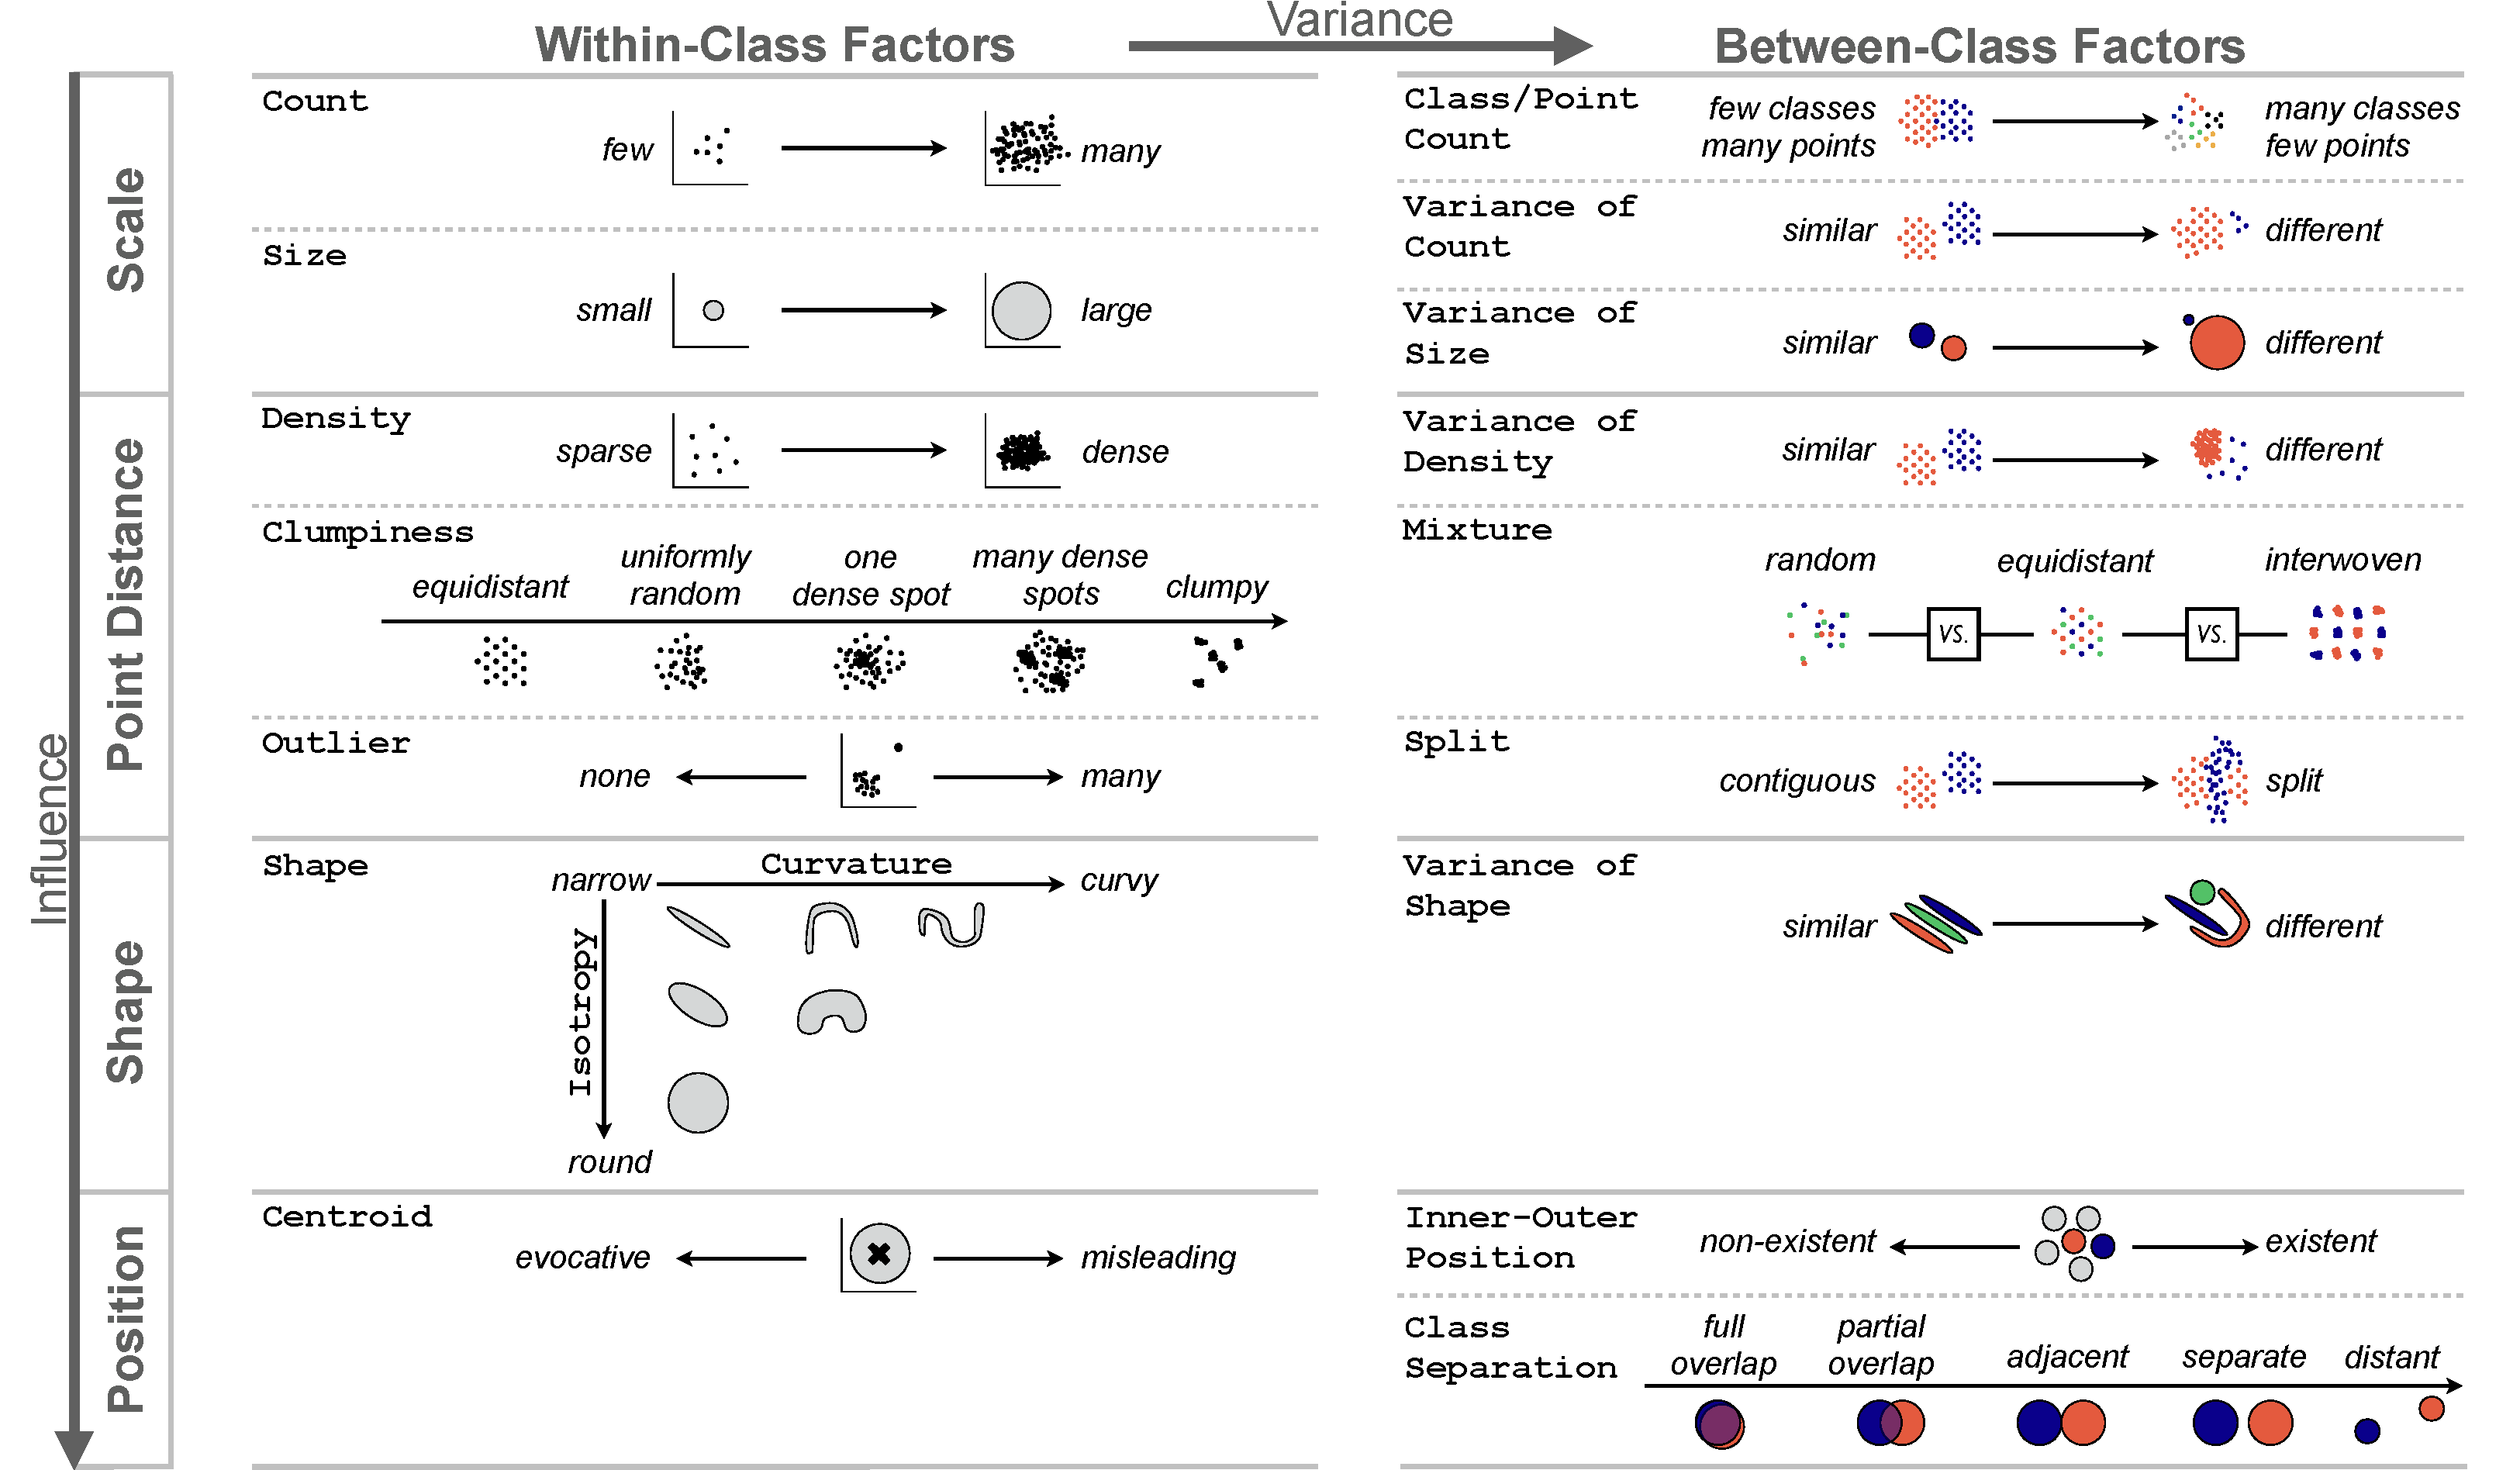
\includegraphics[width=1\textwidth]{images/sedlmair2012taxonomyFull}
\caption{An indirect mapping taxonomy of data characteristics with respect to class separation in scatterplots. Courtesy of Sedlmair et al.\ \cite{sedlmair2012taxonomy}} \label{fig: sedlmair2012taxonomy}
\end{center}
\end{figure}

%\item \textit{Classification Dimensions:}
%\begin{itemize}
%\item[~]\begin{center} Classification Structure: 2D Hierarchical \end{center}
%%\item[List:]
%\item[Y:] Influence
%\item[Y$^1$:] Size: [Count, Size, Class/Point Count, Variance of Count, Variance of Size]
%\item[Y$^2$:] Point Distance: [Density, Clumpiness, Outlier, Variance of Density, Mixture, Split]
%\item[Y$^3$:] Shape: [Shape, Variance of Shape]
%\item[Y$^4$:] Position: [Centroid, Inner-Outer position, Class Separation]
%\item[X:] Within-Class Factors, Between Class Factors.
%
%\item \textbf{Site:} n/a \url{}
%\item \textbf{Papers:} 39 Papers cited in Survey \{1923-2015\}\\

%\end{itemize}

%\item \textit{Unsolved Problems/Future Research:} 
Sedlmair et al.\ suggest that the taxonomy could be extended with new dataset characteristics. 
%\end{enumerate}


%Title: \textit{State of the Art of Performance Visualization} by Isaacs et al.\ \cite{isaacs2014state}.
%\begin{enumerate}
%\item \textit{The Concept:}
Isaacs et al.\ present a survey focused on reviewing hardware and software performance data as well as performance visualization techniques \cite{isaacs2014state}. Performance data is defined as data generated to measure the effectiveness and behavior of a process. The survey develops a taxonomy to aid selection of the appropriate techniques to display performance data for both analysts and developers.
%\item \textit{The Scope:}
They introduce the concepts behind performance visualization, including how it is acquired, what form it can take, and the goals of using performance data. The paper discusses the taxonomy by discussing visualization types based on the source of performance data. Hardware visualization examines performance data of hardware and aims to visualize complex hardware topology. Software visualization describes performance data of software, such as software maintenance. Task performance investigates performance of tasks. The final category, application visualization, discusses context-specific performance data. Isaacs et al.\ also provide an interactive literature browser related to this topic. We provide a full list of these browsers in Table \ref{table:literatureBrowsers}.

%\item \textit{Classification:}
Isaacs et al.\ present their design space by looking at the context, scale and goal of each paper. How each paper fits in the presented taxonomy (hardware, software, task, application), scalability, what it visualizes, and what it presents are discussed (see Figure \ref{fig: isaacs2014state}).

\begin{figure}[p]
\begin{center}
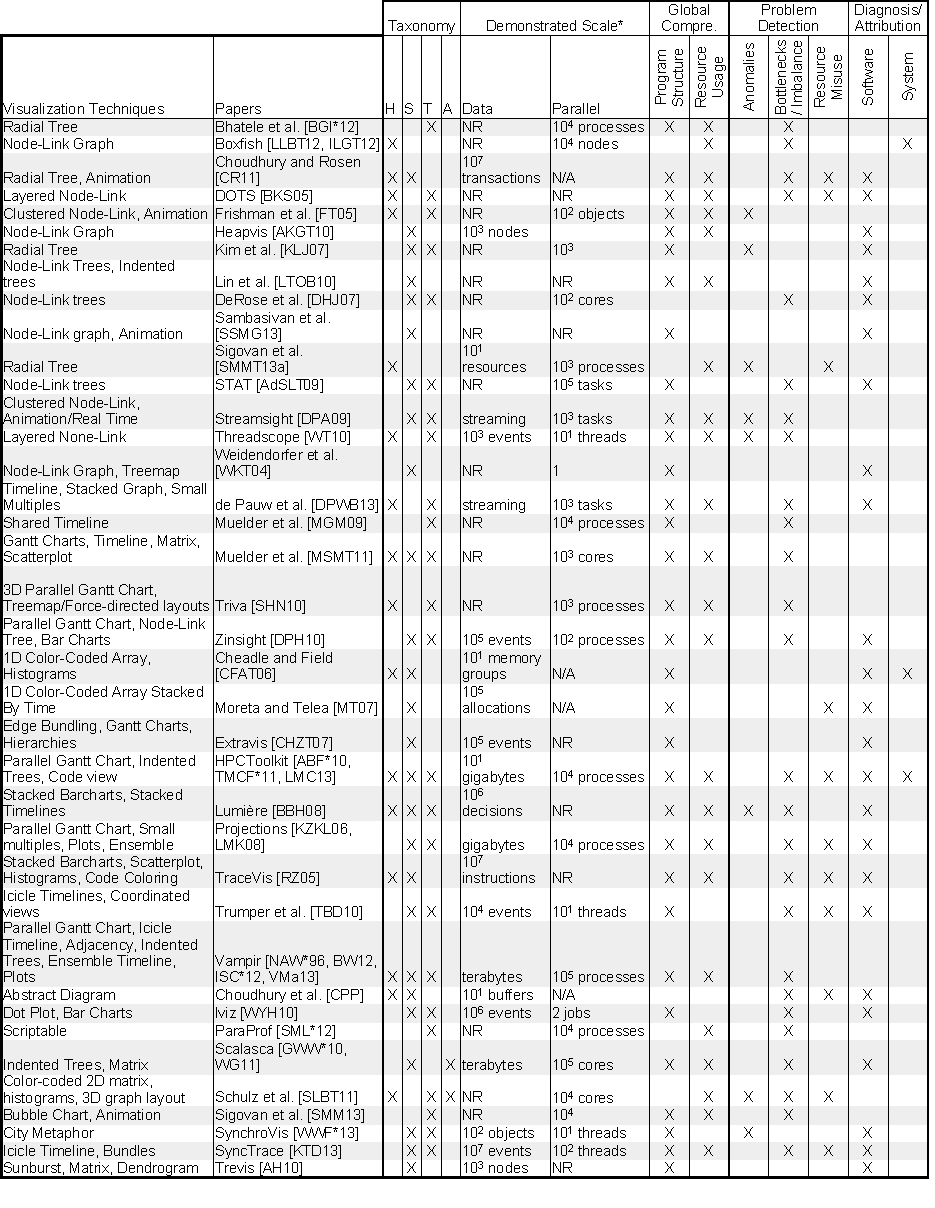
\includegraphics[width=1\textwidth]{images/isaacs2014stateFull}
\caption{Isaacs et al.\ present a 1-N design space that classifies literature based on the context, scale and goal of each paper. Image courtesy of Isaacs et al.\ \cite{isaacs2014state}} \label{fig: isaacs2014state}
\end{center}
\end{figure}

%\item \textit{Classification Dimensions:}
%\begin{itemize}
%\item[~]\begin{center} Classification Structure: 2D Linear \end{center}
%%\item[List:]
%\item[Y:] Techniques
%\item[X$^1$:] Taxonomy: [Hardware, Software, Task, Application]
%\item[X$^2$:] Demonstrated Scale: [Data, Parallel]
%\item[X$^3$:] Global Comprehension: [Program Structure, Resource Usage]
%\item[X$^4$:] Problem Detection: [Anomalies, Bottlenecks and inbalance, Resource Misuse]
%\item[X$^5$:] Diagnosis/Attribution: [Software/System]
%
%\item \textbf{Site:} n/a \url{}
%\item \textbf{Papers:} 108 Papers cited in Survey \{1978-2014\}\\
%
%\end{itemize}

%\item \textit{Unsolved Problems/Future Research:}
The paper presents future challenges that are found within the landscape of performance visualization. These include, scalability, the increase in system complexity and it's result on performance visualization, comparing performance differences and ensemble datasets, integration of performance visualization across each taxonomy point, and the creation of performance visualization that facilitates software development and debugging.

%\end{enumerate}

\begin{table}[] \ra{1.2} \centering \rowcolors{0}{}{black!05} \begin{tabularx}{0.9\linewidth}{|X|c|} %\hline
\hline
\fillCellTitle Interactive Literature Browsers & \fillCellTitle  URLs\\ \hline
Cartogram Visualization & \cite{cartogramVis}\\ 
Dynamic Graph Visualization & \cite{dynamicVis} \\
Financial Visualization & \cite{financeVis} \\
High-Dimensional Visualization & \cite{highdemVis} \\
Matrix Reordering & \cite{matrixreorderingVis}\\
Performance Visualization & \cite{performanceVis} \\
Scientific Literature \& Patents Vis & \cite{litVis} \\
Set Visualization & \cite{setVis} \\
Software Reuse Tasks & \cite{reuseTasks}\\
SoS Literature Browser & \cite{surVis}\\
Space-Time Cube Visualization & \cite{stcVis} \\
Text Visualization & \cite{textVis} \\
Time Visualization & \cite{timeVis} \\
Visualizing Group Structures in Graphs & \cite{groupVis} \\
%-------------------------------------------------------------------------------------------------------% 
\hline \end{tabularx} \caption{%$*$ Surveys not added are: \cite{blackwell1998taxonomy}.
 The tables provides an overview of interactive literature browsers found during the literature search. Sorted in alphabetical order}\label{table:literatureBrowsers} \end{table}


%Title: \textit{A Survey of Colormaps in Visualization} by Zhou and Hansen.\ \cite{zhou2015survey}.
%\begin{enumerate}
%\item \textit{The Concept:}
Zhou and Hansen present a comprehensive review of color-map generation techniques, and provide a reference for readers who are faced with color mapping decisions \cite{zhou2015survey}.
%\item \textit{The Scope:}
The paper aims to provide a comprehensive overview of various color-map generation techniques. The paper also presents a hierarchical taxonomy of color-mapping literature to guide readers when choosing appropriate literature to review, and classifies representative visualization techniques that discuss usage of color-maps.

%\item \textit{Classification:}
The hierarchical classification divides papers into various different color-map generation techniques based on the type of data used in the form of a flow chart. The taxonomy subdivides the data into either discrete or continuous. The discrete data type is split into either nominal or ordinal data types, another division of data comprehension. Both ordinal data and continuous data are linked to color-map transformation literature. The taxonomy also takes into consideration the type of paper and examples.


\begin{figure}[t]
\begin{center}
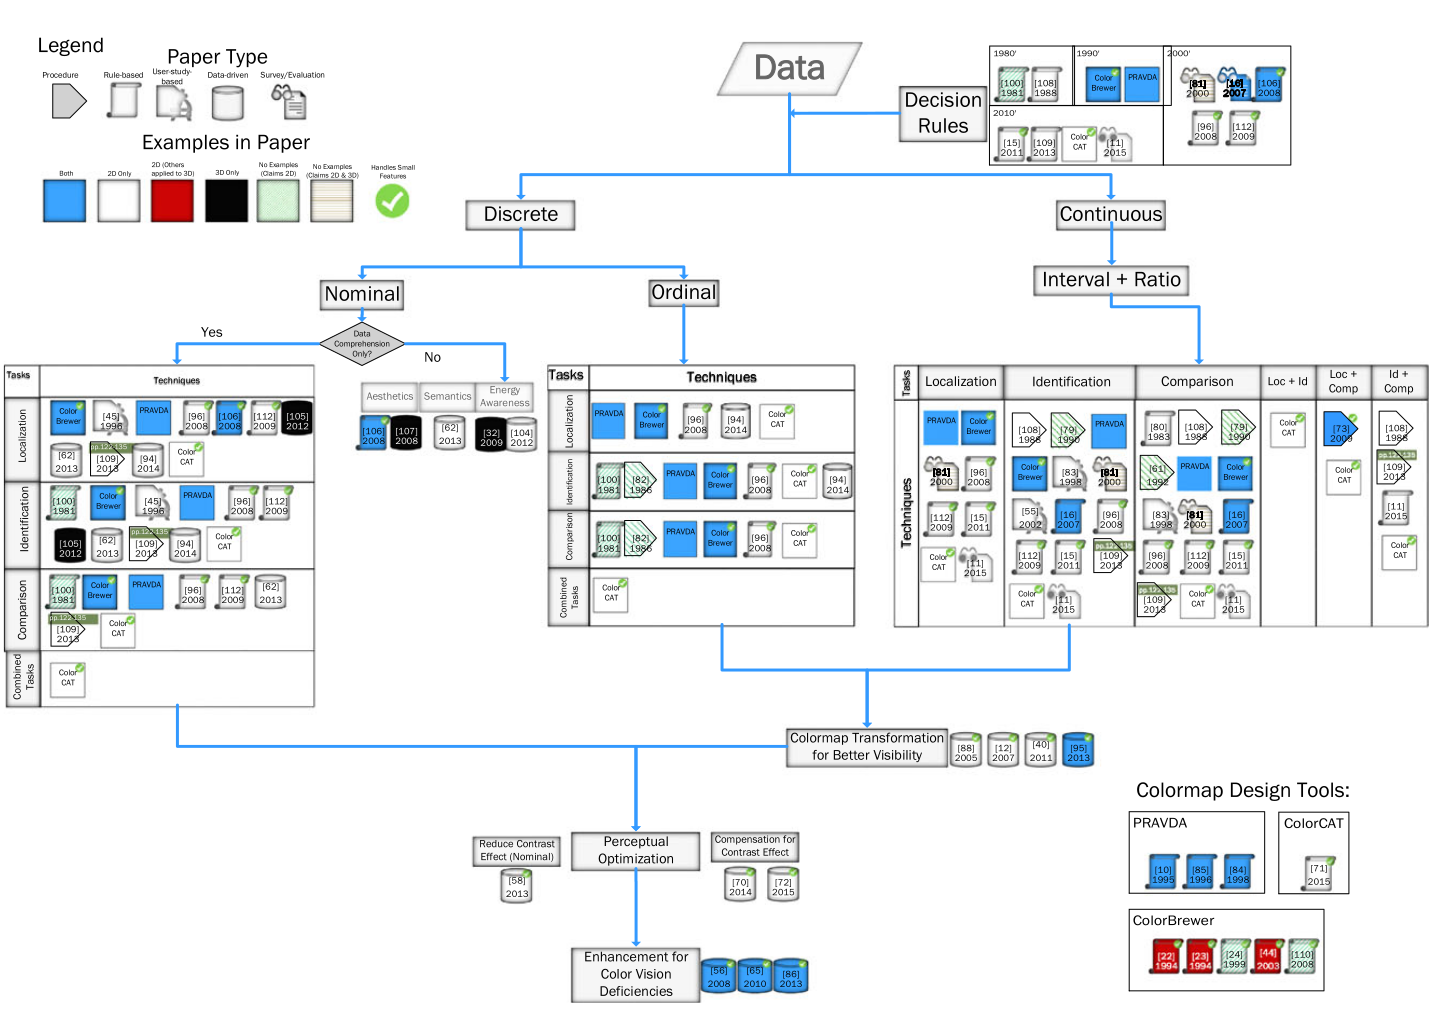
\includegraphics[width=1\textwidth]{images/zhou2015survey}
\caption{The hierarchical taxonomy presents literature by looking at the type of data mapped, and the task of the visualization. The taxonomy uses icons to present the paper-type, and color to signify which examples are present within. Courtesy of Zhou and Hansen \cite{zhou2015survey} .} \label{fig: zhou2015survey}
\end{center}
\end{figure}

%\item \textit{Classification Dimensions:}
%\begin{itemize}
%\item[~]\begin{center} Classification Structure: 4D Hierarchical \end{center}
%%\item[List:]
%\item[X:] Data: [Discrete, Continous]
%\item[Y:] Tasks: [Localization, Identification, Comparison, Combined Tasks, Loc+Id, Loc+Comp, Id+Comp]
%\item[Z$^1$:] Paper Type: [Procedure, Rule-based, User-study, Data driven, Survey/Evaluation]
%\item[Z$^2$:] Examples: [Both, 2D Only, 2D-Focus, 3D Only, No Examples
%\item[\cmark :] Handles small features 
%
%\item \textbf{Site:} n/a \url{}
%\item \textbf{Papers:} 114 Papers cited in Survey \{1942-2015\}\\
%
%\end{itemize}

%\item \textit{Unsolved Problems/Future Research:}
Zhou and Hansen recommend more research into multivariate or high-dimensional color-mapping as a future research direction. Further research into aesthetically pleasing color maps that still provide insight into data, and the use of meta-data to optimize color-mapping suggestions are also potential future research directions in the field.

%\end{enumerate}

\subsubsection{Text-Focused Surveys}
The text visualization literature is evolving rapidly. This section includes surveys focused on understanding and visualizing text. The section contains four survey papers. The first paper analyses how different text sources are used in visualization with event detection methods. The second focuses on advancement in the field of close and distant reading. The third presents a classification of text visualization techniques. The last survey focuses on the visualization of `scientific literature and patent' text sources. Table \ref{table: classificationTableClusters} cites a number of other text surveys as well.

%Title: \textit{State-of-the-art report of visual analysis for event detection in text data streams} by Wanner et al. \cite{wanner2014state}
%\begin{enumerate}
%\item \textit{The Concept:}
With the growth of social media and micro-blogging, Wanner et al.\ take the opportunity to explore the use of analytical processes on real-time data and divulge key event-detection approaches that can be used for textual data \cite{wanner2014state}.
%\item \textit{The Scope:}
They review the different available data sources when working the text-data streams including news, email, micro-blogging, research papers, and metadata. They discuss methods that are used to process text. The study examines the event detection methods that are grouped including: clustering techniques, classification-based, statistic based, and miscellaneous techniques such as the Kalman Filter and Fourier Analysis. They finish  by discussing evaluation methods that can be applied to text-data. 

%\item \textit{Classification:}
Wanner et al.\ classify 51 papers across their survey. They classify these in various ways including: data source, text-processing methods, automatic event detection methods, visualization methods, and tasks supported. The main taxonomy displays the use of automatic event detection methods on the y-axis, and then characterizes each research paper via the visualization technique along the x-axis. By doing this, they can investigate the correlation between these two fields. (Shown in Figure \ref{fig: wanner2014state}).

\begin{figure}[t]
\begin{center}
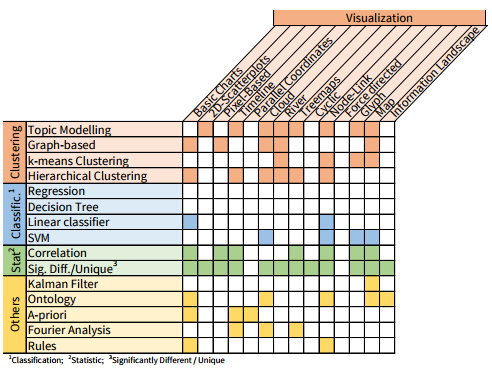
\includegraphics[width=0.8\textwidth]{images/wanner2014state.png}
\caption{This 1-N table identifies event detection techniques and displays the the use of visualization with each. The table reveals that clustering techniques are  often represented using the river metaphor. Image courtesy of Wanner et al.\ \cite{wanner2014state}} \label{fig: wanner2014state}
\end{center}
\end{figure}

%\item \textit{Classification Dimensions:}
%\begin{itemize}
%\item[X:]Visualization:[ Basic Charts, 2D Scatterplots, Pixel-Based, Timeline, Parallel Coordinates, Cloud, River, Treemaps, Cyclic, Node-Link, Force Directed, Glyph, Map, Information Landscape].
%\item[Y:] Clustering, Classification, Statistic, Others. \\
%Topic Modelling, Graph-Based, K-Means Clustering, Hierarchical Clustering, Regression, Decision Tree, Linear Classifier, SVM,Correlation, Significantly Different Unique, Kalman Filter, Ontology, A-Priori, Fourier Analysis, Rules.
%\item \textbf{Papers:} 51 Papers cited in Survey \{1965-2014\}
%\end{itemize}

%\item \textit{Unsolved Problems:}
The reviewed papers had little focus on discussion forums. Demand for more sophisticated techniques such as topic modeling is something that will become more apparent in the future, and event detection algorithms seem to exclude important information for deciding whether items are newsworthy or not. This could be considered new research in this area.
%\end{enumerate}

%Title: \textit{On Close and Distant Reading in Digital Humanities: A Survey and Future Challenges} by Janicke et al.\ 
%\begin{enumerate}
%\item \textit{The Concept:}
J{\"a}nicke et al.\ present recent advancements in the field of visualizations that support close and distant reading of textual data \cite{janicke2015on}. Nancy Boyles defines close reading as "reading to uncover layers of meaning that lead to deep comprehension" \cite{boyles2012closing}, whilst Moretti describes distant reading with the statement, "a little pact with the devil: we know how to read texts, now let's learn how not to read them" \cite{moretti2013distant}. The paper focuses on quantitative literary text analysis using statistical analysis methods for visual analytics and visualization. Literature in the digital humanities is also covered. These are categorized using a taxonomy for applied methods \cite{janicke2015on}.
%\item \textit{The Scope:}
The paper looks at different types of techniques, such as color mapping or heat-maps, for close-reading analysis, distant-reading analysis, and combinations of both.

%\item \textit{Classification:}
J{\"a}nicke et al.\ classify papers based on the type of reading analysis provided, which is broken down for each paper. This is compared to the method of analysis, which includes single text analysis, parallel-text analysis, and corpus analysis.

\begin{figure}[p]
\begin{center}
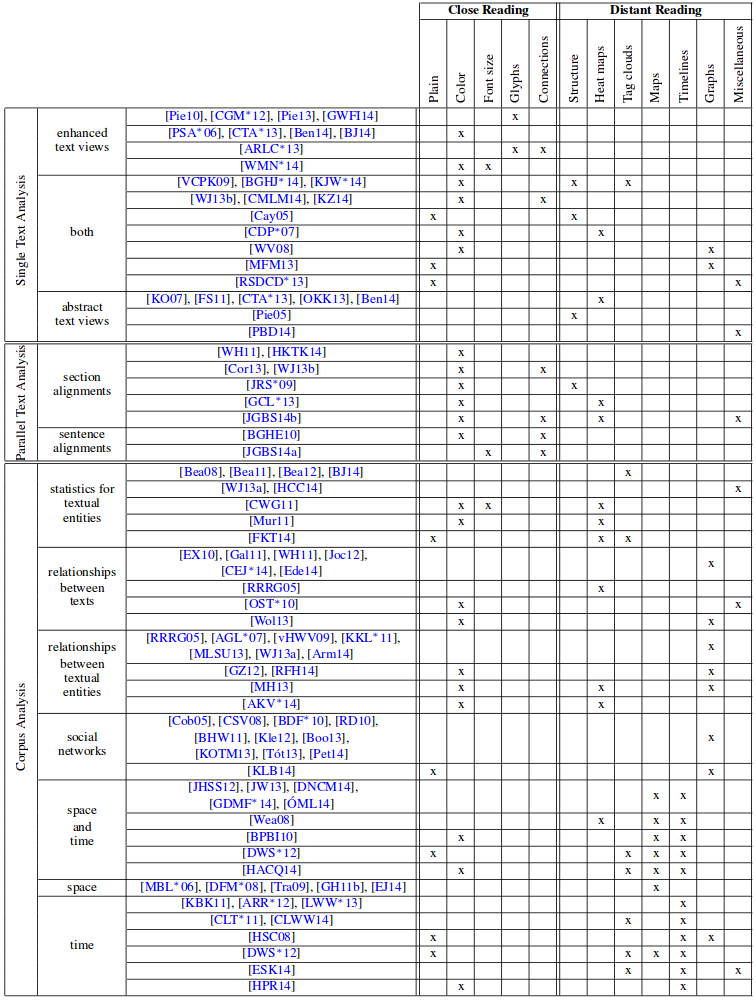
\includegraphics[width=1\textwidth]{images/janicke2015on}
\caption{A 1-N Taxonomy by J{\"a}nicke et al.\ to map reading techniqes found within different analysis methods. Image courtesy of Janicke et al.\ \cite{janicke2015on}} \label{fig: janicke2015on}
\vspace{-0.3cm}
\end{center}
\end{figure}

%\item \textit{Classification Dimensions:}
%\begin{itemize}
%\item[~]\begin{center} Classification Structure: 2D Hierarchical \end{center}
%%\item[List:]
%\item[X$^1$:] Single-Text Analysis: [Enhanced text views, abstract text view, both]
%\item[X$^2$:] Parallel-Text Analysis: [Section Alignments, Sentence Alignments]
%\item[X$^3$:] Corpus Analysis: [statistics for textual entities, relationships between texts, relationships between textual entities, social networks, space and time, space, time]
%\item[Y$^1$:] Close Reading: [Plain, Color, Font Size, Glyphs, Connections]
%\item[Y$^2$:] Distant Reading: [Structure, Heat maps, tag clouds, maps, timelines, graphs, miscellaneous]
%\item \textbf{Url: } n/a \url{}
%\item \textbf{Papers: } 162 Papers cited in Survey \{1996-2015\}\\
%
%\end{itemize}

%\item \textit{Unsolved Problems/Future Research:}
They provide a large collection of areas for future research which includes novel techniques for close reading, visualizing transposition in parallel texts, geospatial and temporal uncertainty, usability studies, and the development of design guidelines for scholars. All these areas are ripe with unsolved problems in the field. J{\"a}nicke et al.\ published an extended version of this survey \cite{janicke2016visual}.
%\end{enumerate}

%Title: \textit{Text Visualization Techniques: Taxonomy, Visual Survey, and Community Insights} by Kucher et al.\ \cite{kucher2015text}
%\begin{enumerate}
%\item \textit{The Concept:}
Text visualization is becoming a more mature field within information visualization and Kucher and Kerren aim to classify the literature using an interactive browser \cite{kucher2015text}. See also Table \ref{table:literatureBrowsers}.
%\item \textit{The Scope:}
They examine the field of text visualization and closely related surveys. Kucher and Kerren then present the taxonomy they have created to look at different areas within text visualization and how they can be subdivided (the figure is provided in the supplementary material).

%\item \textit{Classification:}
Kucher and Kerren categorize text visualization techniques into 5 main categories: Analytic Tasks, Visualization Tasks, Domain, Data, and Item Visualization.


\begin{figure}[t]
\begin{center}
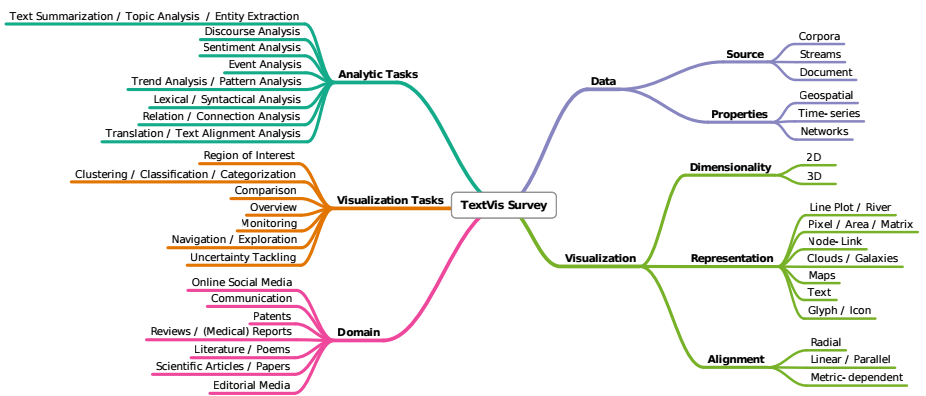
\includegraphics[width=1\textwidth]{images/kucher2015text}
\caption{Kucher et al.\ present a hierarchical taxonomy used to classify text visualization techniques \cite{kucher2015text}  .} \label{fig: kucher2015text}
\end{center}
\end{figure}

%\item \textit{Classification Dimensions:}
%\begin{itemize}
%\item[~]\begin{center} Classification Structure: Hierarchical \end{center}
%%\item[List:]
%\item[1:] Analytic Tasks: [Text Summary, Discourse Analysis, Sentiment Analysis, Event Analysis, Trend Analysis, Lexical, Relation, Translation]
%\item[2:] Visualization Tasks: [Region of Interest, Clustering, Comparison, Overview, Monitoring, Navigation, Uncertainty]
%\item[3:] Domain: [Social Media, Communication, Patents, Reviews, Literature, Scientific Articles, Editorial Media]
%\item[4:] Data: [Corporate, Streams, Document, Geospatial, Time-series, Networks]
%\item[5:] Visualization: [2D, 3D, Line Plot, Pixel, Node-Link, Clouds, Maps, Text, Glyph, Radial, Linear, Metric-Dependent]
%
%
%\item \textbf{Site:} \url{http://textvis.lnu.se/}
%\item \textbf{Papers:} 35 Papers cited in Survey \{1992-2015\}\\
%
%\end{itemize}

%\item \textit{Unsolved Problems/Future Research:}
%n/a (Short Paper)

%\end{enumerate}

%Title: \textit{A Survey on Visual Approaches for Analyzing Scientific Literature and Patents} by Federico et al.\ \cite{federico2016survey}.
%\begin{enumerate}
%\item \textit{The Concept:}
Federico et al.\ present a survey that addresses literature papers with an emphasis on visual approaches for scientific literature and patents. Literature is classified looking at the data-type and the fulfilled task of each \cite{federico2016survey}.
%\item \textit{The Scope:}
The paper identifies four types of data found within scientific literature papers and patents. These include text, citations, authors, and meta-data. The data types create the main structure of the paper, with each data-type divided to explore how tasks are analyzed for each category. The paper also provides a breakdown of literature that handles multiple data types, which focus on different tasks.

%\item \textit{Classification:}
Their indirect classification uses two tables. The first table displays the total number of publications that match the criteria at the axis intersections, which examine the four data-types and different tasks such as lookups, relation seeking, and patterns. The second table is similar but records how multiple data-types are mapped to a new set of tasks. This includes aggregation, labeling, composition, tight integration, and multiple views. The table shows that most literature in the field attempts to analyze patterns within text.

\begin{figure}[t]
\begin{center}
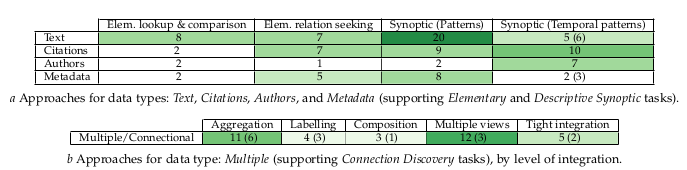
\includegraphics[width=1\textwidth]{images/federico2016survey}
\caption{Table \textit{a} presents the distribution of papers for each single data category, whilst \textit{b} contains the distribution papers which look at multiple data-types. Both tables distribute papers based on  tasks. Numbers in parentheses are papers identified as a secondary classification. Image courtesy of Federico et al.\ \cite{federico2016survey} .} \label{fig: federico2016survey}
\end{center}
\end{figure}

%\item \textit{Classification Dimensions:}
%\begin{itemize}
%\item[~]\begin{center} Classification Structure: 2D Linear \end{center}
%%\item[List:]
%\item[X:] Tasks
%\item[Y:] Data-Type
%\item[Z:] Colour: Visual Aid
%
%\item \textbf{Site:} \url{http://www.paperviz.org}
%\item \textbf{Papers:} 151 Papers cited in Survey \{1977-2016\}\\
%
%\end{itemize}

%\item \textit{Unsolved Problems/Future Research:}
Federico et al.\ break down future research directions for each data-type. Research on text data identifies contextual identification in compact space. Research into author data suggests uncertainty analysis of ambiguities with synonyms and homonyms. Limited work is provided with citation data and meta-data, with citation data focusing on citation count and meta-data ignoring many pieces of gathered data, which narrows the fields significantly. Some other broader examples include quantitative and qualitative evaluations, scalability, user interaction, and research into user-tasks.

%\end{enumerate}

\subsection{Multivariate \& Hierarchical}
This category discusses multivariate, high-dimensional, and hierarchical visualization. These are grouped together due to their association within large datasets. The reviewed content on this subject can be broken down to look at hierarchical visualization, an overview of high-dimensional visualizations, parallel coordinate plots, and glyph-based visualization.
\subsubsection{Hierarchical Surveys}
This section includes surveys that have an emphasis on hierarchical structures. The first survey focuses on the classification of hierarchical aggregation strategies for visualization. The second survey provides a design space of implicit hierarchy visualization to compare literature in the field. The final survey looks at set-typed data and how set-typed data visualizations relate to different tasks.

%Title: \textit{Hierarchical Aggregation for Information Visualization: Overview, Techniques, and Design Guidelines} by Elmqvist and Fekete. \cite{elmqvist2010hierarchical}.
%\begin{enumerate}
%\item \textit{The Concept:}
Elmqvist and Fekete review the use of hierarchical aggregation within Information Visualization. Hierarchical Aggregation is based on iteratively building a tree of aggregate items. Elmqvist and Fekete use this review to present a model that enables augmentation of existing techniques with multiscale functionality \cite{elmqvist2010hierarchical}.
%\item \textit{The Scope:}
They first describe related reading  before discussing hierarchical aggregation and presenting various related techniques (scatter-plots, parallel coordinates, etc). The paper then presents examples of hierarchical aggregation within visualization before presenting their classification and guidelines (the figure is provided in the supplementary material). Elmqvist and Fekete end by describing design guidelines for hierarchical aggregation.

%\item \textit{Classification:}
Elmqvist and Fekete derive a classification of visual aggregation strategies. The table looks at the data-structure used, visualization mapping type, type of visualization, type of aggregation, the visual  aggregate, and what is being visualized.

\begin{figure}[t]
\begin{center}
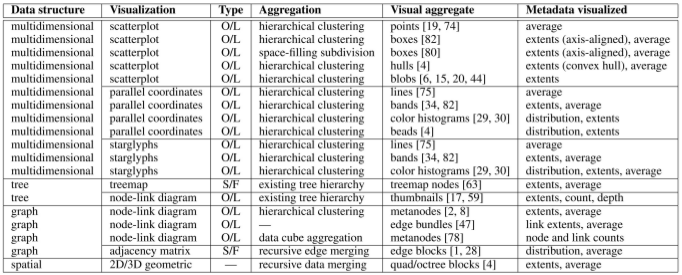
\includegraphics[width=1\textwidth]{images/elmqvist2010hierarchical}
\caption{A hierarchical classification of aggregation strategies for Information Visualization techniques. Image courtesy of Elmqvist and Fekete \cite{elmqvist2010hierarchical} .} \label{fig: elmqvist2010hierarchical}
\end{center}
\end{figure}

%\item \textit{Classification Dimensions:}
%\begin{itemize}
%\item[~]\begin{center} Classification Structure: Hierarchical \end{center}
%
%\item[X$^1$:] Data Structure: [multidimensional, tree, graph, spatial]
%\item[X$^2$:] Visualization: [scatterplot, parallel coordinates, starglyphs, treemap, node-link diagram, adjacency matrix, 2D/3D geometric]
%\item[X$^3$:] Type: [Overlapping, Space-Filling]
%\item[X$^4$:] Aggregation: [Hierarchical Clustering, Space-Filling Subdivision, Existing Tree Hierarchy, Data Cube Aggregation, Recursive Edge Merging, Recursive Data Merging]
%\item[X$^5$:] Visual Aggregate: [points, boxes, hulls, blobs] 
%\item \textbf{Site:} n/a \url{}
%\item \textbf{Papers:} 60 Papers cited in Survey \{1983-2010\}\\
%
%\end{itemize}

%\item \textit{Unsolved Problems/Future Research:}
Elmqvist and Fekete discuss future work which includes model refinements, as well as investigating the trade-off between accuracy and usability. Finally, they look at the idea of reviewing different hierarchical structures such as Directed Acyclic Graphs (DAGs).
%\end{enumerate}

%Title: \textit{The Design Space of Implicit Hierarchy Visualization: A Survey} by Schulz et al.\ \cite{schulz2011design}.
%\begin{enumerate}
%\item \textit{The Concept:}
Schulz et al.\ construct a survey categorizing the design space of techniques for hierarchy visualization, with the aim of guiding researchers to unexplored research areas within the field \cite{schulz2011design}. Examples of techniques for implicit hierarchy visualization include spatial dimensions and node representation.
%\item \textit{The Scope:}
Schulz et al.\ present their aims, before presenting the design space for hierarchy visualization (see Figure \ref{fig: shulz2011design}). They follow this by discussing some of the limitations of the design space such as techniques with \textit{mixed Treemaps}. Using the design space, they present novel techniques that are not explored with visual representations, using their own rapid visualization prototyping software.

%\item \textit{Classification:}
The survey paper investigates four main classification topics. Spatial dimensionality, how nodes are represented (such as their shape), how edges are represented (Do they overlap? Are they included?), and the layout (subdivision or packing).

\begin{figure}[p]
\begin{center}
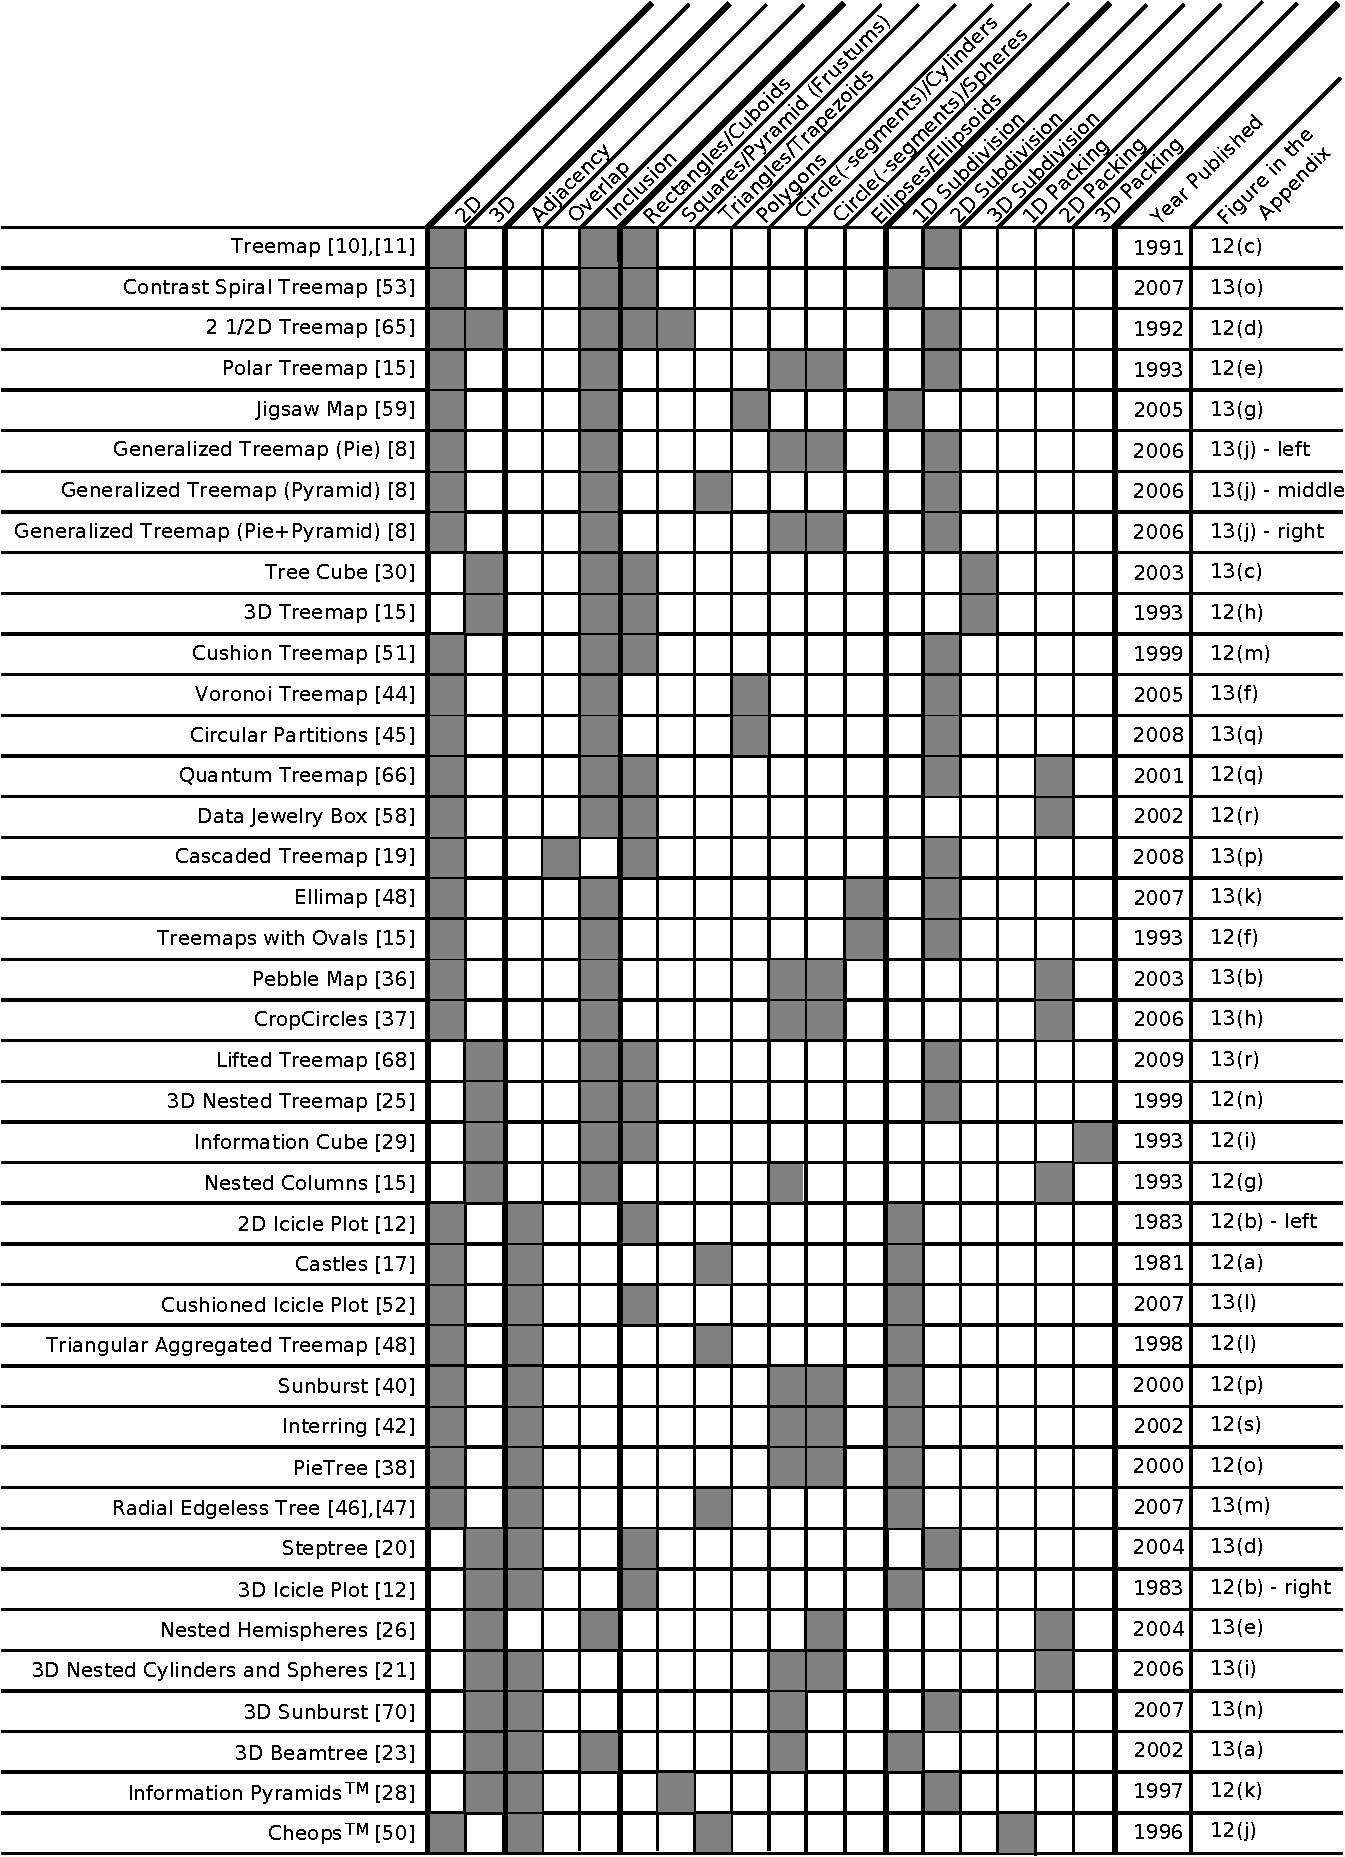
\includegraphics[width=0.9\textwidth]{images/schulz2011designFull}
\caption{Design space for implicit hierarchy visualization created by Schulz et al.\ to compare techniques in the field. Image courtesy of Schulz et al.\ \cite{schulz2011design}} \label{fig: shulz2011design}
\end{center}
\vspace{-0.5cm}
\end{figure}

%\item \textit{Classification Dimensions:}
%\begin{itemize}
%\item[~]\begin{center} Classification Structure: 2D Hierarchical \end{center}
%%\item[List:]
%\item[Y:] Techniques
%\item[X$^1$:] Dimensionality: [2D,3D]
%\item[X$^2$:] Edge Representation: [Adjacency, Overlap, Inclusion]
%\item[X$^3$:] Node Representation: [Rectangles/Cuboids, Squares/Pyramid (Frustrums), Triangles/Trapezoids, Polygons, Circle/Cylinders], Spheres, Ellipses]
%\item[X$^4$:] Layout: [1D Subdivision, 2D Subdivision, 3D Subdivision, 1D Packing, 2D Packing, 3D Packing]
%\item[X:] Year Published.
%
%\item \textbf{Site:} n/a \url{}
%\item \textbf{Papers:} 79 Papers cited in Survey \{1969-2011\}\\
%
%\end{itemize}

%\item \textit{Unsolved Problems/Future Research:}
Schulz et al.\ propose that the design space presented in the paper can be used to create more surveys within the field of hierarchy visualization. New layouts can also be created using the characterization of implicit hierarchy visualization.

%\end{enumerate}

%Title: \textit{Visualising Sets and Set-Typed Data} by Alsallakh et al. \cite{alsallakh2014visualising}
%\begin{enumerate}
%\item \textit{The Concept:}
Visualization of sets can be a demanding task due to the wide variety of possible relations between them. Sets are defined as items that are grouped into sets based on specific properties. Alsallakh et al.\ present an overview of state-of-the-art techniques for visualizing different forms of set data (defined as a collection of unique objects called set elements) which can be used to select appropriate techniques for different scenarios \cite{alsallakh2014visualising}.
%\item \textit{The Scope:}
They first define set-type data before looking at some common tasks. The tasks are either related to elements, element attributes, or relationships between sets. The paper then provides examples of different ways to visualize set-typed data such as using euler diagrams, bubble-sets, pivot-paths, and scatter views.

%\item \textit{Classification:}
Alsallakh et al.\ classify literature by constructing an overview of different tasks and techniques that are supported, partially supported, or supported with an interaction requirement. These techniques include Euler-based techniques, overlays, node-link's, matrices, aggregation, and scatter techniques (the figure is provided in the supplementary material).

\begin{figure}[p]
\begin{center}
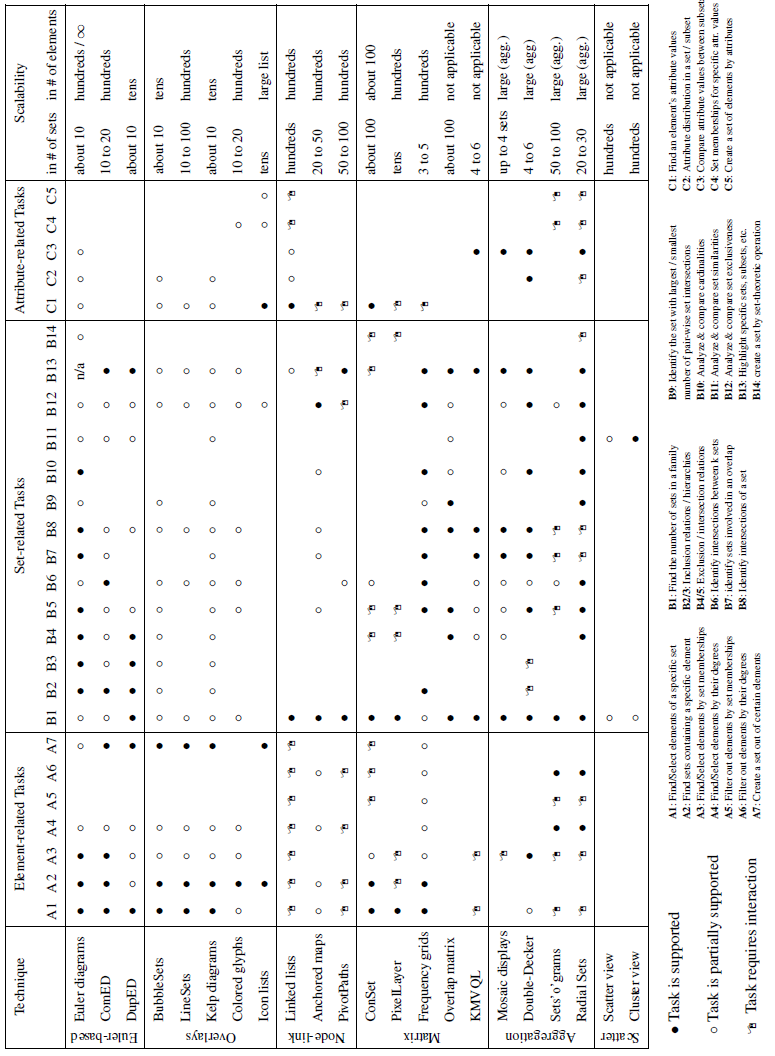
\includegraphics[width=1\textwidth]{images/alsallakh2014visualising}
\caption{A 1-N taxonomy of set-types data showing a comparision between tasks and techniques. Courtesy of Alsallakh et al.\ \cite{alsallakh2014visualising}} \label{fig: alsallakh2014visualising}
\end{center}
\end{figure}

%\item \textit{Classification Dimensions:}
%\begin{itemize}
%\item[X:] Tasks: [Element-Related Tasks, Set-Related Tasks, Attribute-Related Tasks]
%\item[Y:] Techniques: [Euler-Based, Overlays, Node-Link, Matrix, Aggregation, Scatter]
%\item[Z:] Support-Type: [Supported, Partially-Supported, Requires Interaction, Not Supported]
%\item \textbf{Papers:} 106 Papers cited in Survey \{1935-2015\}\\
%\end{itemize}

%\item \textit{Unsolved Problems/Future Research:}
The paper presents an abundance of future research in this area. These include scalability within set-typed data, re-ordering sets to reveal clusters, a user study on the effectiveness of techniques, visualizing uncertainty, temporal set-typed data, generating euler diagrams with specific properties, visualizing set in context of other data types, and comparing multiple set families. There is also a discussion of improvements with coordinated multiple views and matrix-based representations of set-type data.

%\end{enumerate}

\subsubsection{High-Dimensional Surveys}
The high-dimensional section focuses on surveys that provide a broad overview of the field of high-dimensional visualization. "High-Dimensional" is defined as `any data set with a dimensionality that is too high to easily extract meaningful relations across the whole set of dimensions' by Bertini et al.\ \cite{bertini2011quality}. The section covers two surveys papers. The first paper reviews quality metrics for high-dimensional visualization. The second survey discusses the recent advancements for visualization of high-dimensional data.

%Title: \textit{Quality Metrics in High-Dimensional Data Visualization: An Overview and Systematization} by Bertini et al.\ \cite{bertini2011quality}.
%\begin{enumerate}
%\item \textit{The Concept:}
Bertini et al.\ review techniques that use quality metrics, defined as \textit{"a metric calculated at any stage of the information visualization pipeline, that captures properties useful for the extraction of meaningful information about the data"}, to find meaningful results for the exploration of high-dimensional data. By analyzing literature related to the topic, Bertini et al.\ provide a systematization of approaches that use quality metrics in high-dimensional data. \cite{bertini2011quality}.
%\item \textit{The Scope:}
They begin by describing the background and search methodology used within the survey. The paper presents the quality metrics pipeline, a modified version of Card et al.'s information visualization pipeline \cite{card1999readings}, which we also use, before discussing their systematic analysis of the literature. Bertini et al.\ then give examples of quality metrics factors such as what is measured, where, and its purpose.

%\item \textit{Classification:}
The survey classifies each work of literature by examining the visualization technique, the metrics measured which range from clusters to image quality, where the measurements take place, the purpose of the metrics, and any interaction techniques available.

\begin{figure}[p]
\begin{center}
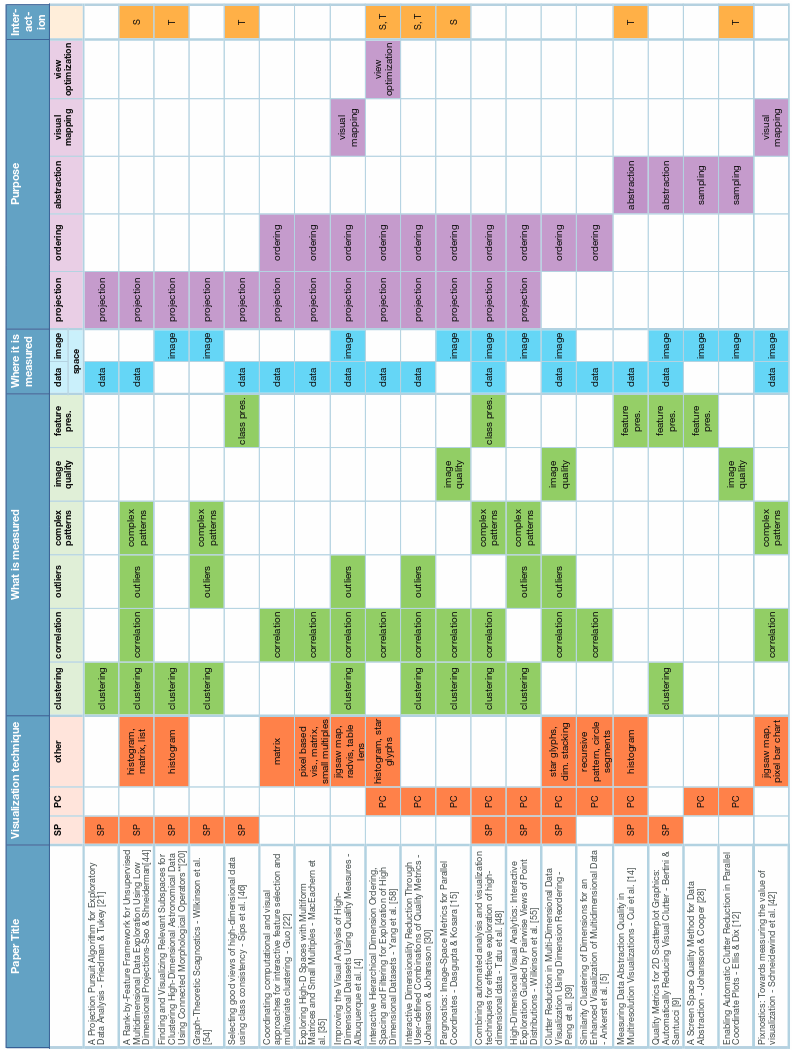
\includegraphics[width=1\textwidth]{images/bertini2011quality}
\caption{A 1-N classification created to systemise quality metrics factors for high-dimensional data. Courtesy of Bertini et al.\ \cite{bertini2011quality}} \label{fig: bertini2011quality}
\end{center}
\end{figure}

%\item \textit{Classification Dimensions:}
%\begin{itemize}
%\item[~]\begin{center} Classification Structure: 2D \end{center}
%
%\item[X$^1$:] Visualization Technique: [Scatter Plot, Parallel Coordinates, Other]
%\item[X$^2$:] What is Measured: [Clustering, Correlation, Outliers, Complex Patterns, Image Quality, Feature Presentation]
%\item[X$^3$:] Where it is measured: [Data, Image, Space]
%\item[X$^4$:] Purpose: [Projection, Ordering, Abstraction, Visual Mapping, View Optimization]
%\item[X$^5$:] Interaction: [Select Metric, Set Threshold] 
%\item \textbf{Site:} n/a \url{}
%\item \textbf{Papers:} 60 Papers cited in Survey \{1974-2011\}\\
%
%\end{itemize}

%\item \textit{Unsolved Problems/Future Research:}
Four main areas for future research are highlighted in the paper. Evaluation is poorly represented within the field with a small representation of the papers using a real-world setting and data. This could pave a path for future research. Perceptual Tuning is another area with weak focus, as well as scalability of data representation. Metrics systematization is the final area for directed future research. There are a wealth of different metrics which makes them very hard to compare and without guidance could end up as redundant metrics usage. Composite visualization of quality metrics is also discussed.
%\end{enumerate}

%Title: \textit{Visualising High-Dimensional Data - Advances in the Past Decade} by Liu et al. \cite{liu2015visualising}
%\begin{enumerate}
%\item \textit{The Concept:}
Liu et al.\ provide a comprehensive survey focused on the advances of high-dimensional visualization techniques between 2000 and 2014 \cite{liu2015visualising}. The study aims to help practitioners understand the recent advances in this area with the hope of inspiring the creation of new visualizations and the comprehension of future opportunities with high-dimensional data.
%\item \textit{The Scope:}
They first discuss their classification and methodology before discussing various sections or the information visualization pipeline. Similar to ours, this includes data transformation, visual mapping, and view transformation.

%\item \textit{Classification:}
The taxonomy of the survey is based on the information visualization pipeline (the figure is provided in the supplementary material). The classification clearly represents when techniques are to be used within the pipeline, as well as some action-driven classification signifying the time of use for each technique. Some examples of this are histograms, jigsaw maps, and glyphs. Liu et al.\ have also created custom action-driven classifications to further improve their taxonomy.

\begin{figure}[t]
\begin{center}
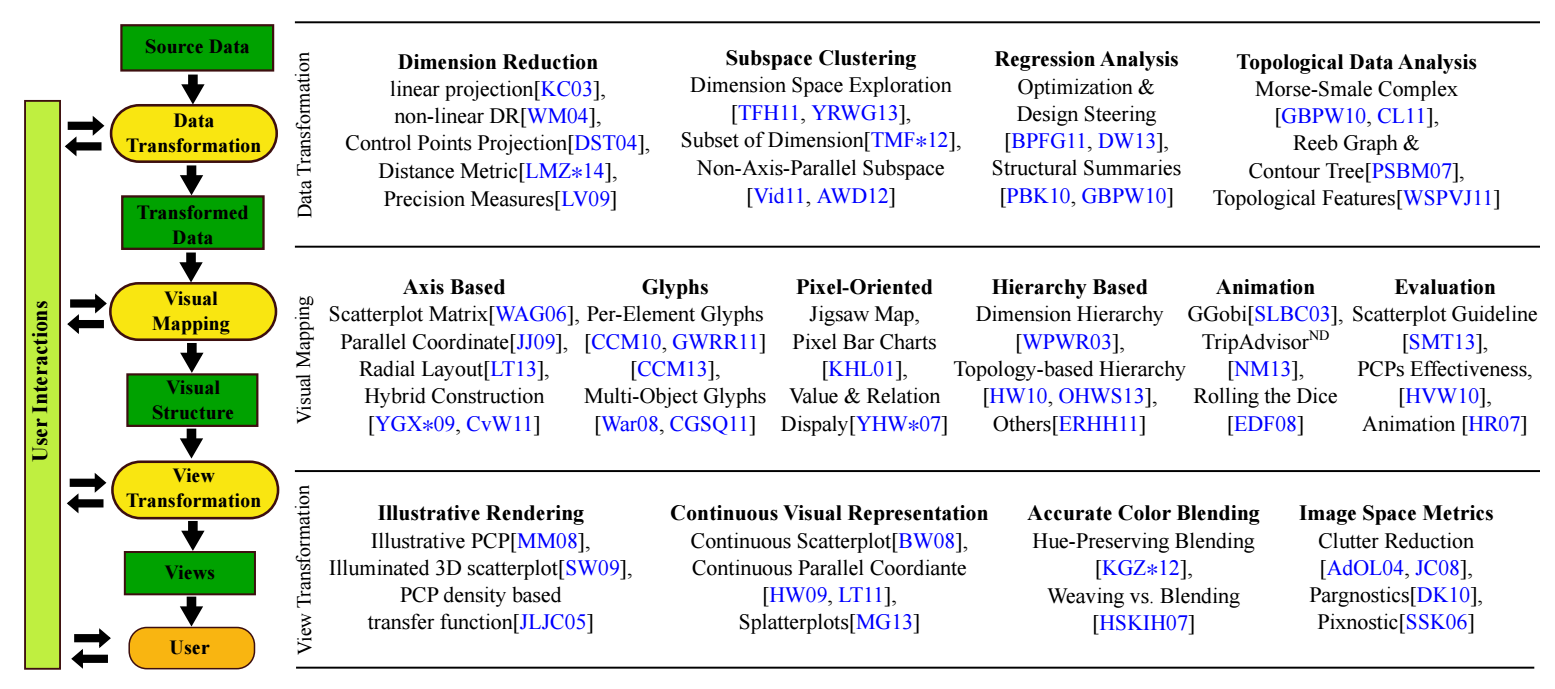
\includegraphics[width=1\textwidth]{images/liu2015visualising.png}
\caption{A 2D classification designed using the information visualization pipeline for the taxonomy of high dimensional data. Courtesy of Liu et al.\ \cite{liu2015visualising}} \label{fig: liu2015visualising}
\end{center}
\end{figure}

%\item \textit{Classification Dimensions:}
%\begin{itemize}
%\item[X:] Customised Subcategories: [Dimension Reduction, Subspace Clustering, Regression Analysis, Topological Data Analysis], 
%
%[Axis Based, Glyphs, Pixel-Oriented, Hierarchy Based, Animation, Evaluation],
%
%[Illustrative Rendering, Continuous Visual Representation, Accurate Color Blending, Image Space Metrics]
%\item[Y:] Visualization Pipeline: [Data Transformation, Visual Mapping, View Transformation]
%\item \textbf{Papers:} 215  Papers cited in Survey \{1974-2014\}\\
%
%\end{itemize}

%\item \textit{Unsolved Problems/Future Research:}
Liu et al.\ take great care to expose multiple directions for future research. Subspace clustering is an important technique used when visualizing high-dimensional data, and exploring non-axis-aligned methods may lead to new view-selection techniques. Understanding uncertainty within data is also an important research area. As the amount of data increases, so does the understanding of the quality of data and the best way to visualize this high-dimensional data will become more apparent. Liu et al.\ also discuss model manipulation, topological data analysis, as well as problems occurring with multivariate volume visualization and machine learning with a link to high-dimensional data visualization.

%\end{enumerate}
\subsubsection{Parallel Coordinates Surveys}
Parallel Coordinates are a technique used to visualize multivariate and high-dimensional data. Parallel coordinates are constructed by placing axes in parallel, the choice of layout depends on the number of axes, and the range of data \cite{heinrich2013state}. Included here are two survey papers focusing on Parallel Coordinates. One focuses on the design and structure of Parallel Coordinates and the second collects the findings of user-evaluation studies, comparing the use of a standard 2D parallel coordinate plot with other variations.


%Title: \textit{State of the Art of Parallel Coordinates} by Heinrich et al.\ \cite{heinrich2013state}.
%\begin{enumerate}
%\item \textit{The Concept:}
Heinrich and Weiskopf present the state of the art in visualization techniques for parallel coordinates, which is well-known for exploratory data analysis \cite{heinrich2013state}. The paper describes the parallel coordinate plane, and reviews different variations of the methodology, with the hope of directing research in new areas related to the topic.
%\item \textit{The Scope:}
The paper aims to provide (1) a taxonomy of techniques related to parallel coordinates, (2) a review of challenges in the field, (3) a reference to important literature in the domain, and (4) a guide to the use of parallel coordinates for applications.

%\item \textit{Classification:}
Heinrich and Weiskopf split their hierarchical taxonomy into four main topics: Geometry which focuses on the coordinate system creation; Image Generation maps data to the coordinate system; Image Analysis highlights visual perception of the mapped parallel coordinate; and Interaction emphasizes manipulation of the parallel coordinates (see Figure \ref{fig: heinrich2013state}).

\begin{figure*}[t]
\begin{center}
\includegraphics[width=1\textwidth]{images/heinrich2013stateFull}
\caption{An indirect hierarchical taxonomy of important topics withn Parallel Coordinate creation. Created by Heinrich and Weiskopf, the taxonomy reflects the different sections of their survey. Courtesy of Heinrich and Weiskopf \cite{heinrich2013state} .} \label{fig: heinrich2013state}
\end{center}
\end{figure*}

%\item \textit{Classification Dimensions:}
%\begin{itemize}
%\item[~]\begin{center} Classification Structure: Hierarchical \end{center}
%%\item[List:]
%\item[1:] Geometry: [Projective Geometry, Interpolation]
%\item[2:] Image Generation: [Samples, Axes]
%\item[3:] Image Analysis: [Automatic, Human]
%\item[4:] Interaction: [Samples, Axes]
%
%
%\item \textbf{Site:} n/a \url{}
%\item \textbf{Papers:} 149 Papers cited in Survey \{1885-2013\}\\
%
%\end{itemize}

%\item \textit{Unsolved Problems/Future Research:}
They state that an evaluation of existing tools would be required to identify issues in the implementation of parallel coordinate techniques. Additionally, more in-depth studies can test each category in order to find underrepresented research areas. They avoid evaluating techniques based on their applicability, correctness, usability, and performance. These are considered areas for future work within the field.
%\end{enumerate}

%Title: \textit{Evaluation of Parallel Coordinates: Overview, Categorization and Guidelines for Future Research} by Johansson and Forsell.\ \cite{johansson2016evaluation}.
%\begin{enumerate}
%\item \textit{The Concept:}
Johansson and Forsell provide a thorough literature review survey studying user-centered evaluations that investigate use and usability issues in the field of parallel coordinates. The paper aims to address issues within the domain and provide a set of guidelines for future research \cite{johansson2016evaluation}.
%\item \textit{The Scope:}
They first divide the 23 papers identified into 4 categories: evaluating axis layouts, comparing clutter reduction methods, showing practical applicability of different parallel coordinates, and comparing parallel coordinates with other analysis techniques. These categories are discussed in detail with reference to the evaluated papers.  The categories include cluster analysis, correlation analysis, outlier search, value retrieval, pattern detection, and line tracing.

%\item \textit{Classification:}
The paper provides a classification of how each paper compares with standard 2D Parallel Coordinates (2DPC). The table (provided in the supplementary material) maps the selection of aspects evaluated. The third dimension uses color to indicate how the advanced feature compares to a standard 2D Parallel Coordinates: Yellow identifies no significance variation in the results, Green signifies the extension is reviewed to be better than 2DPC, and red signifies the reviewed item compares unfavorably with 2DPC.


\begin{figure}[ht]
\begin{center}
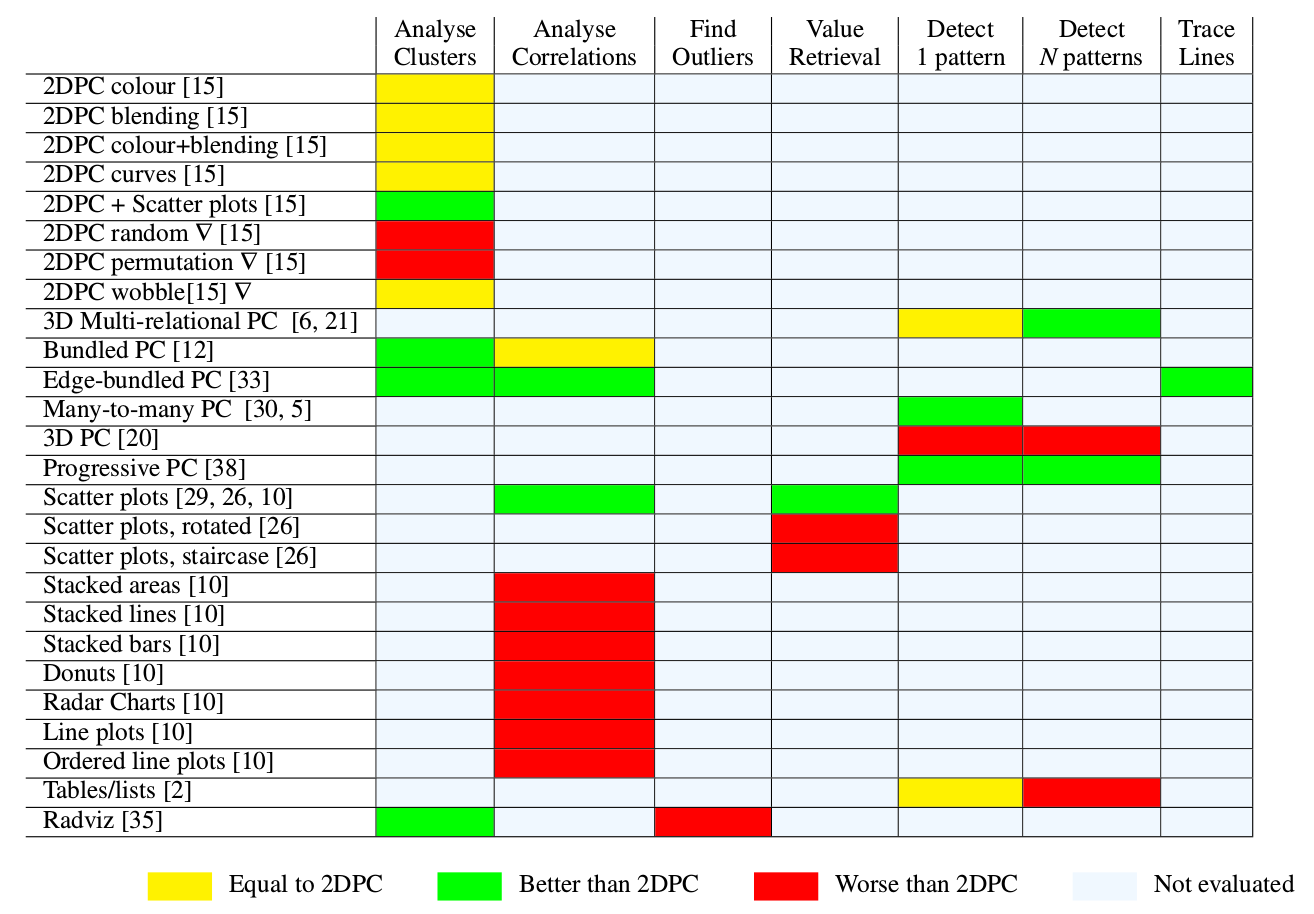
\includegraphics[width=1\textwidth]{images/johansson2016evaluation}
\caption{A 1-N classification of 26 techniques performed in relation to standard 2D parallel coordinates. Yellow colour indicates no significant difference in performance. Green colour means that the technique outperforms 2DPC for the specific task. Red colour shows the technique performs worse than 2DPC. Light blue colour reveals no evaluation has been found in the literature. $\nabla$ denotes that the technique is based on animation. Courtesy of Johansson and Forsell \cite{johansson2016evaluation} .} \label{fig: johansson2016evaluation}
\end{center}
\end{figure}

%\item \textit{Classification Dimensions:}
%\begin{itemize}
%\item[~]\begin{center} Classification Structure: 2D Linear \end{center}
%%\item[List:]
%\item[Y:] Identified Techniques
%\item[X:] Evaluation Tasks: [Analyse Clusters, Analyse Correlations, Find Outliers, Value Retrieval, Detect 1 Pattern, Detect N Patterns, Trace Lines]
%\item[Z:] Performance against 2DPC: [Equal, Better, Worse]
%\item[$\nabla$:] Animation
%
%\item \textbf{Site:} n/a \url{}
%\item \textbf{Papers:} 50 Papers cited in Survey \{1952-2014\}\\
%
%\end{itemize}

%\item \textit{Unsolved Problems/Future Research:}
Johansson and Forsell provide a plethora of different research directions in the field. The paper proposes that existing axis configurations in parallel coordinate plots have not been thoroughly studied, with an emphasis on 3D parallel coordinates. They discuss the lack of conclusive clutter reduction comparisons, and propose research in evaluating clutter reduction for complex patterns in parallel coordinates. Some other areas for future research discussed include longitudinal studies, temporal views in 3D parallel coordinates, and the aesthetic design of parallel coordinates.

%\end{enumerate}

\subsubsection{Glyph Surveys}
A glyph is defined as  \textit{`a small independent visual object that depicts attributes of a data record'} \cite{borgo2013glyph}. Glyphs use visual primitives to represent different attributes in multivariate data. This section contains two literature surveys. The first presents design guidelines for the creation of glyphs. The second paper presents a selection of glyph comparison papers to provide an evaluative perspective on glyph usage.

%\begin{figure}[h]
%\begin{center}
%\includegraphics[width=0.45\textwidth]{images/glyphExamples}
%\caption{Examples of different glyph designs by Fuchs et al.\ \cite{fuchs2016systematic}}
%\end{center}
%\end{figure}

%Title: \textit{Glyph-based Visualization: Foundations, Design Guidelines, Techniques and Applications} by Borgo et al. \cite{borgo2013glyph}
%\begin{enumerate}
%\item \textit{The Concept:}
Borgo et al.\ examine the fundamental concepts and design guidelines of glyph-based visualization, and how current implementation techniques adhere to them  \cite{borgo2013glyph}.
%\item \textit{The Scope:}
They first discuss the concepts and history of glyph usage. The paper covers the design and usage guidelines for glyphs, data mapping, shape design, glyph appearance, glyph placement, rendering, and glyph interaction. Borgo et al.\ then discuss the application of glyph-based visualization in different visualization scenarios.

%\item \textit{Classification:}
Borgo et al.\ categorize the literature by examining each technique and determining whether they fulfill the design guideline criteria. There are 13 tasks created that the papers are categorized according to, which range from complexity and prioritization to design and balance. The papers are also categorized according to the focus on different visual channels including color, shape, size, orientation, texture, and opacity (see Figure \ref{fig: borgo2013glyph}).

\begin{figure}[t]
\begin{center}
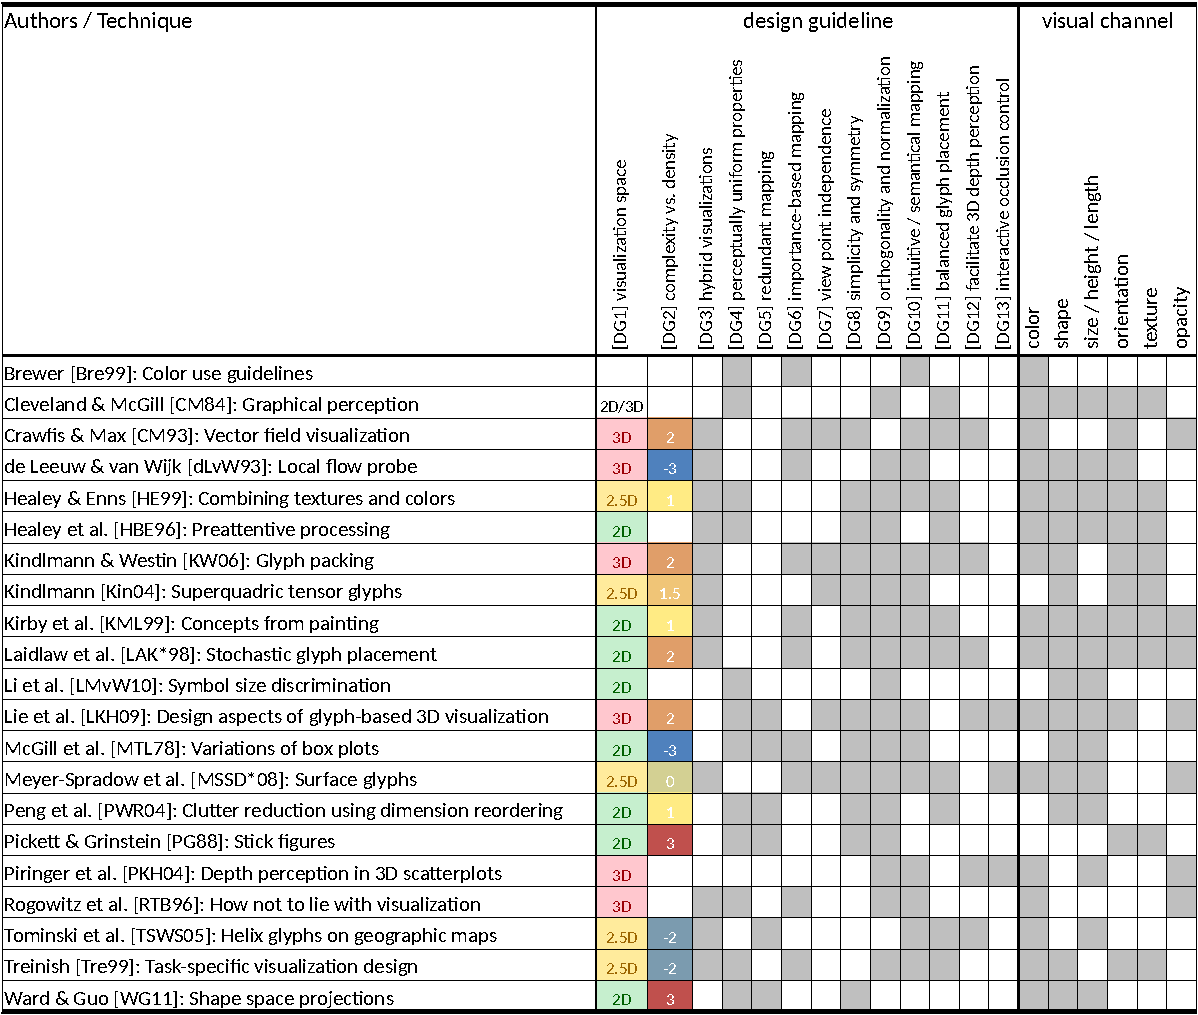
\includegraphics[width=1\textwidth]{images/borgo2013glyphFull}
\caption{A 1-N categorization of glyph-based approaches created by Borgo et al. In Desgin Guideline 2, -3 represents a small amount of complex glyphs with +3 displaying a large number of simple glyphs. Courtesy of Borgo et al.\ \cite{borgo2013glyph}} \label{fig: borgo2013glyph}
\end{center}
\end{figure}

%\item \textit{Classification Dimensions:}
%\begin{itemize}
%\item[Y:] Authors/Techniques
%\item[X$^1$:] Design Guideline: [Visualization Space, Complexity vs Density, Hybrid Visualizations, Perceptually uniform properties, redundant mapping, importance-based mapping, view point independence, simplicity and symmetry, orthogonality and normalisation, intuitive/semantical mapping, balanced glyph placement, facilitate 3D depth perception, interactive occlusion control]
%\item[X$^2$:] Visual Channel: [Color, Shape, Orientation, Size/Height/Length, Texture, Opacity]
%\item \textbf{Papers:} 130 Papers cited in Survey \{1964-2013\}\\
%\end{itemize}

%\item \textit{Unsolved Problems/Future Research:}
Borgo et al.\ suggest the need for a common framework to direct more energy to the field. They also suggest evaluating extended data dimensions using glyph representations.
%\end{enumerate}

\begin{figure}[p]
\begin{center}
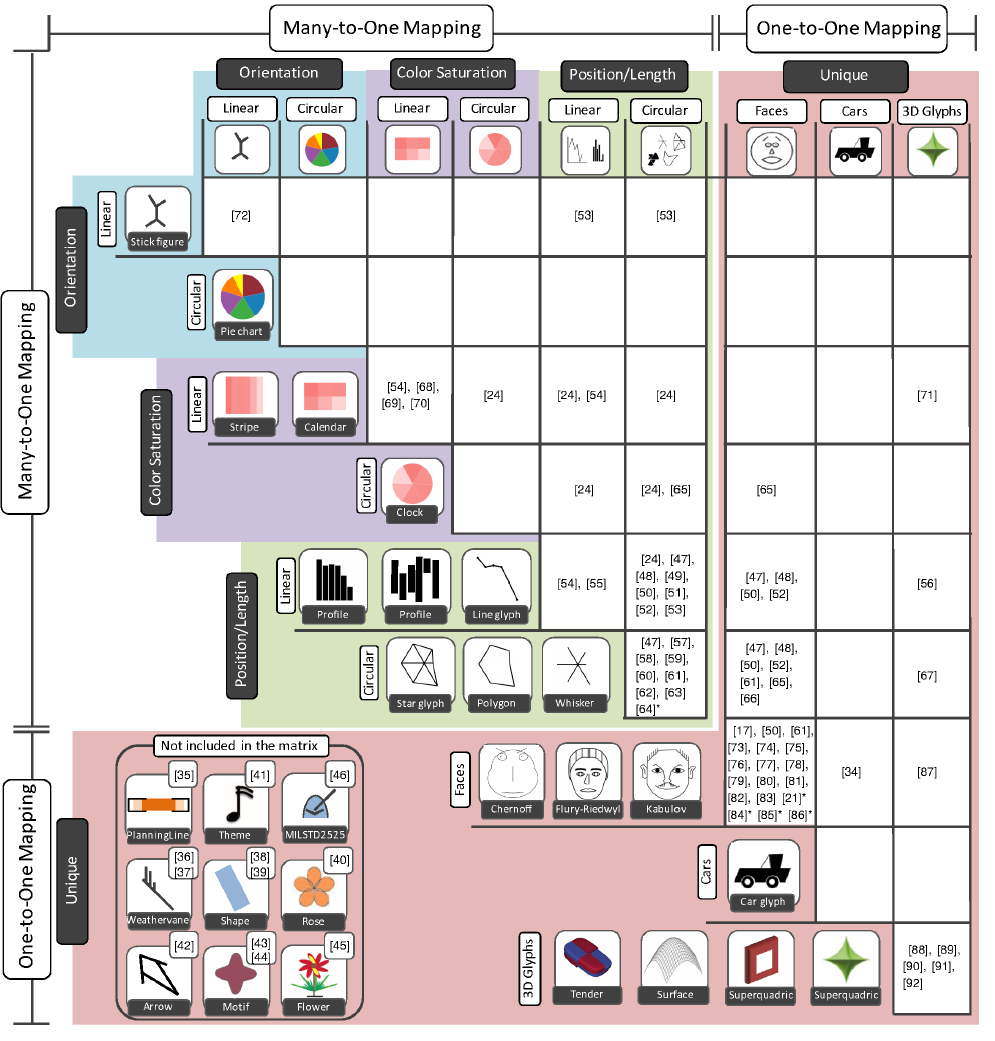
\includegraphics[width=1\textwidth]{images/fuchs2016systematic.png}
\caption{A 2-Dimensional table showing the classification of the literature in the glyph-based user-study survey. Courtesy of Fuchs et al.\ \cite{fuchs2016systematic}} \label{fig:fuchs2016systematic}
\end{center}
\end{figure}
%Title: \textit{A Systematic Review of Experimental Studies on Data Glyphs} by Fuchs et al. \cite{fuchs2016systematic}
%\begin{enumerate}
%\item \textit{The Concept:}
Fuchs et al.\ aim to assist researchers in gaining a stronger understanding of user-studies within the glyph design space \cite{fuchs2016systematic}. Data glyphs have a wide variety of designs and uses, with many studies carried out across different glyph-types, however an overview of these studies has never been recorded. They present how the expanse of user-studies in the field compare. There are many types of data glyphs analyzed within the paper including: orientation-based, which include angular representations to represent dimensions; color saturation, which uses various saturation's to represent dimension values; positional or length glyphs, which plot dimensional data to bars or lines; and Faces, which map dimensional data to different attributes of a face. 
%\item \textit{The Scope:}
They focus on studies with measurable tasks using data glyphs. Tasks are discussed within the classification. The three main goals identified are 1) a comparison of glyph designs based on observed performance with the aim of ranking each design. 2) A comparison of variation within glyph types to detect important features within the data type. 3) The comparison of glyphs as opposed to raw data tables in order to stimulate the use of visual representation rather than textual representations \cite{fuchs2016systematic}. Fuchs et al.\ present the results of their survey by reviewing the influence of background information or the layout, the quantity of data, data dimensionality, the influence of the task, and the effect of metaphoric glyph design.

%\item{Classification: }
The literature is classified according to data-to-visual primitive mapping. This classification allows Fuchs et al.\ to understand some comparisons with limited discussion and discuss the benefits of further work within the area (see Figure \ref{fig:fuchs2016systematic}).

\begin{figure*}[t]
\begin{center}
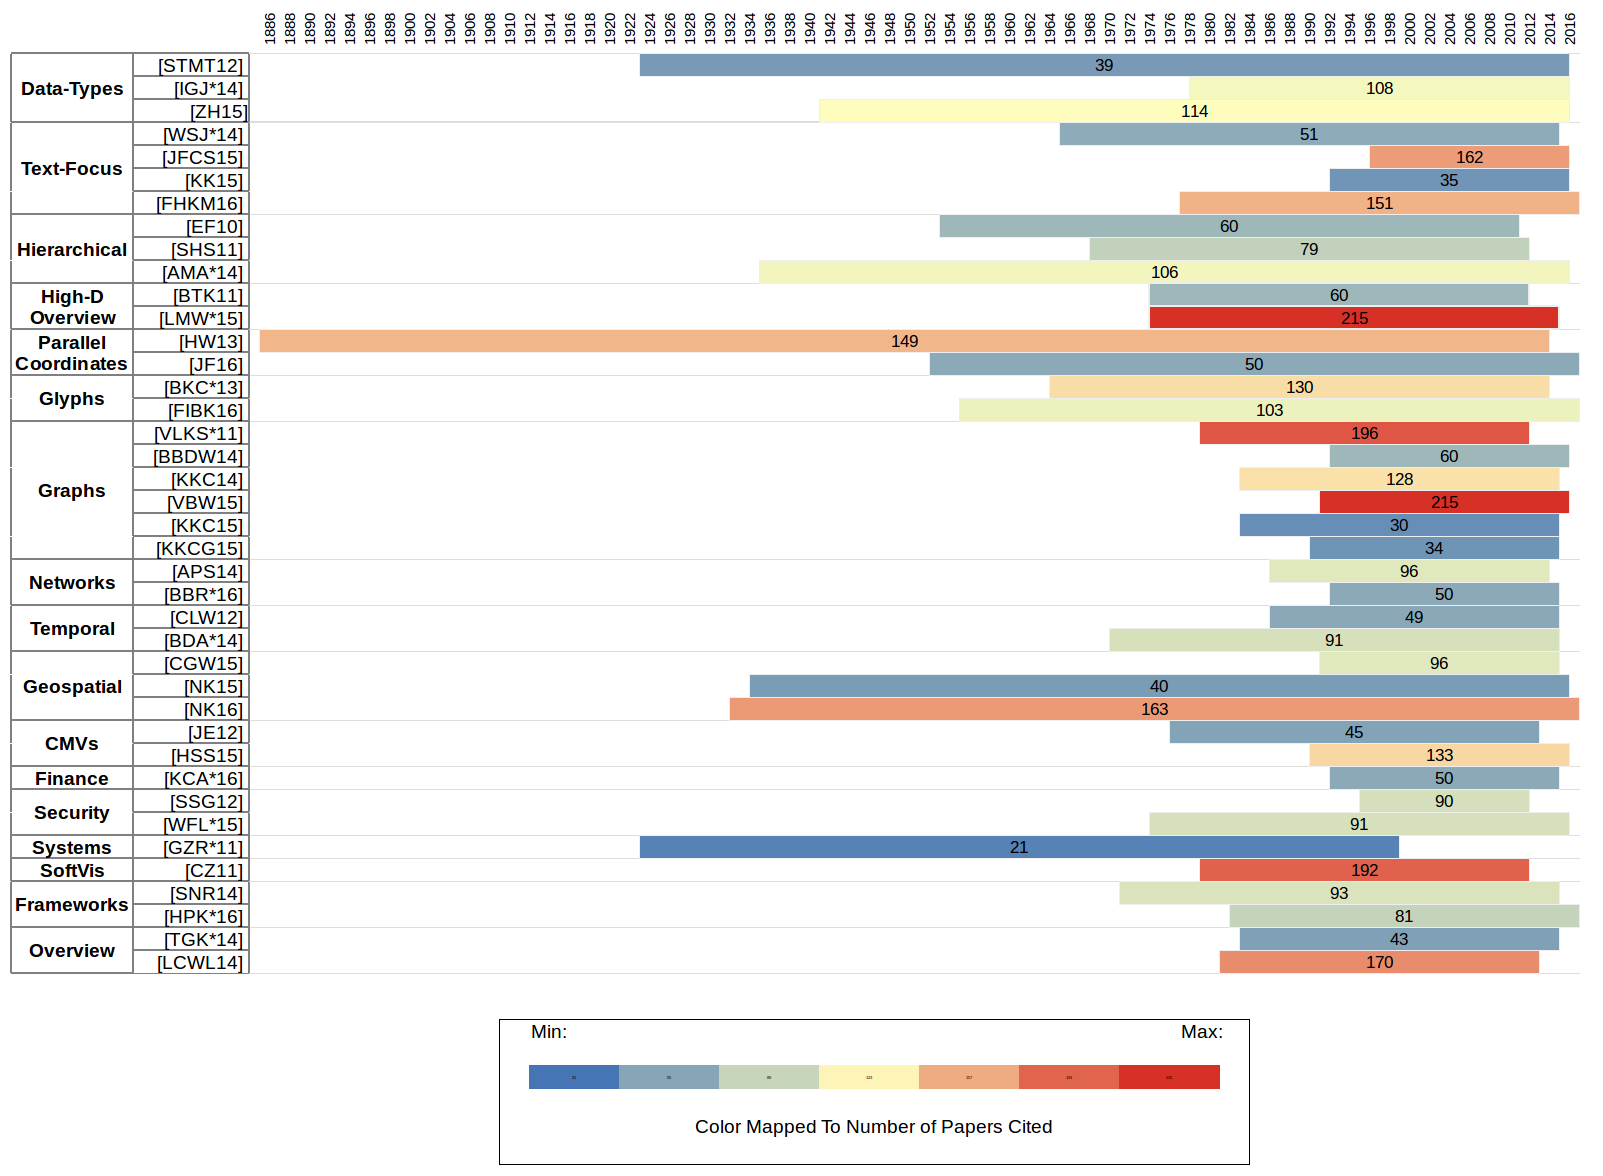
\includegraphics[width=1\textwidth]{images/citationvis5}
\caption{Visualization of the number of citations within each survey paper discussed, where the years spanned is mapped to the length of each bar along the x-axis. The color represents the number of papers cited within each survey.} \label{fig: citationvis}
\end{center}
\end{figure*}

%\item \textit{Classification Dimensions: }
%\begin{itemize}
%\item[X:]Glyph Type, Layout, Number of Dimensions,\\ Task type: [Lookup, 3D Navigation, Trend Detection, Similarity Search, Visual Search].
%\item[Y:]Type: [Single Glyph; Multiple Glyphs; Varying Glyphs.]
%\item \textbf{Papers:} 103 Papers cited in Survey
%\end{itemize}

%\item \textit{Unsolved Problems: }
Fuchs et al.\ provide many open research areas within their survey. There is a large contrast in the observations of data glyphs for quantitative data compared to observations with qualitative data. There is also little research on how data glyphs differ between synthetic and real data. Fuchs et al.\ find a high percentage of studies fail to look at the use of data-glyphs in exploring data and extracting information, but focus on presentation and simple output in it's stead. They propose that data glyphs can be explored in more complex layouts in order to understand further use and glyph influence in applications.
%\end{enumerate}

\subsection{Graphs \& Networks}
There is a large body of work published on graphs and networks with over 10 surveys about the topic. Graph papers tend to have a concise range of citation years, which can be seen in Figure \ref{fig: citationvis}. This figure shows the quantity and range of citations found for each survey paper.


\subsubsection{Graph Surveys}
This section includes surveys with a focus on graph papers. A graph is defined as \textit{`a diagram showing the relation between variable quantities'} \cite{sedig2016design}. The section includes six survey papers: an analysis of large graphs, a classification of dynamic graphs, the visualization of grouped structures in graphs, and three papers providing an understanding of temporal graph visualization.

%Title: \textit{Visual Analysis of Large Graphs: State-of-the-Art and Future Research Challenges} by Von Landesberger et al.\ \cite{von2011visual}.
%\begin{enumerate}
%\item \textit{The Concept:}
Von Landesberger et al.\ examine the visual analysis of graphs designed for large data sets. The survey reviews current techniques, with regards to the types of graph supported, and aims to present open research challenges in the field \cite{von2011visual}.
%\item \textit{The Scope:}
They give some key definitions for graphs and preprocessing techniques that are related to the survey, including different types of graphs (directed, dynamic, compound, etc.). They introduce some visual representations of these graphs, as well as how interaction in graphs is incorporated. Von Landesberger et al.\ finish the survey with graph analysis.

%\item \textit{Classification:}
Von Landesberger et al.\ classify graphs according to both time-dependency and structure. Time dependency can be split into either static graphs, or time-dependent graphs, whilst the structure can be classified as a tree structure, generic graph structure (directed, undirected) or compound graphs (the figure is provided in the supplementary material).

\begin{figure}[t]
\begin{center}
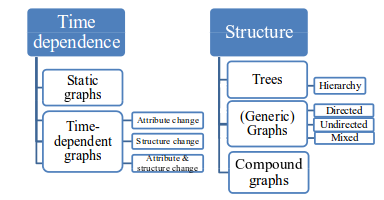
\includegraphics[width=0.7\textwidth]{images/von2011visual}
\caption{Classification of graphs with respect to the temporal or structural characteristics. Courtesy of Von Landesberger et al.\ \cite{von2011visual} .} \label{fig: von2011visual}
\end{center}
\end{figure}

%\item \textit{Classification Dimensions:}
%\begin{itemize}
%\item[~]\begin{center} Classification Structure: Hierarchical \end{center}
%%\item[List:]
%\item[1:] Time Dependence: [Static Graphs, Time-Dependenct Graphs]
%\item[1$^2$:] Time-Dependenct Graphs: [Attribute Change, Structure Change, Attribute \& Structure Change]
%\item[2:] Structure: [Trees, Generic Graphs, Compound Graphs]
%\item[2$^2$:] Generic Graphs: [Undirected, Directed, Mixed]
%
%
%\item \textbf{Site:} n/a \url{}
%\item \textbf{Papers:} 196 Papers cited in Survey \{1979-2011\}\\
%
%\end{itemize}

%\item \textit{Unsolved Problems/Future Research:}
They provide extensive insight into the future challenges within the field. These include scalability, uncertainty, perceptual evaluation, interaction, task evaluation, data-type analysis, generic frameworks, user studies, and graphing benchmark systems.
%\end{enumerate}

%Title: \textit{Visualising The State of the Art in Visualising Dynamic Graphs} by Beck et al.\ \cite{beck2014state}
%\begin{enumerate}
%\item \textit{The Concept:}
Using the SurVis system \cite{beck2016visual}, Beck et al.\ create a paper deriving a hierarchical taxonomy of dynamic graph visualization which is achieved by categorizing and tagging publications within the area, as well as evaluating and comparing the use of animated diagrams against time-line diagrams (see Table \ref{table:literatureBrowsers}). The paper first classifies a static graph as $G := (V,E)$, where \textit{V} represents the vertices and \textit{E} defines the edges. Understanding this allows a representation of a dynamic graph as $G_{i} := (V_{i}, E_{i})$, where \textit{i} defines the number of time steps for the graph \cite{beck2014state}. The paper could also be considered a survey within our temporal categorization.
%\item \textit{The Scope:}
The three main section discussed are animation, time-lines, and a hybrid of the two  (the figure is provided in the supplementary material).

%\item \textit{Classification:}
The hierarchical classification of dynamic graph visualization provides the density of reviewed papers per category, as well as some example techniques for each subsection. Beck et al.\ also provide an interactive system using SurVis \cite{beck2016visual} to provide extra categorization for user-exploration of the dynamic graph visualization field.

%\begin{figure}[ht]
%\begin{center}
%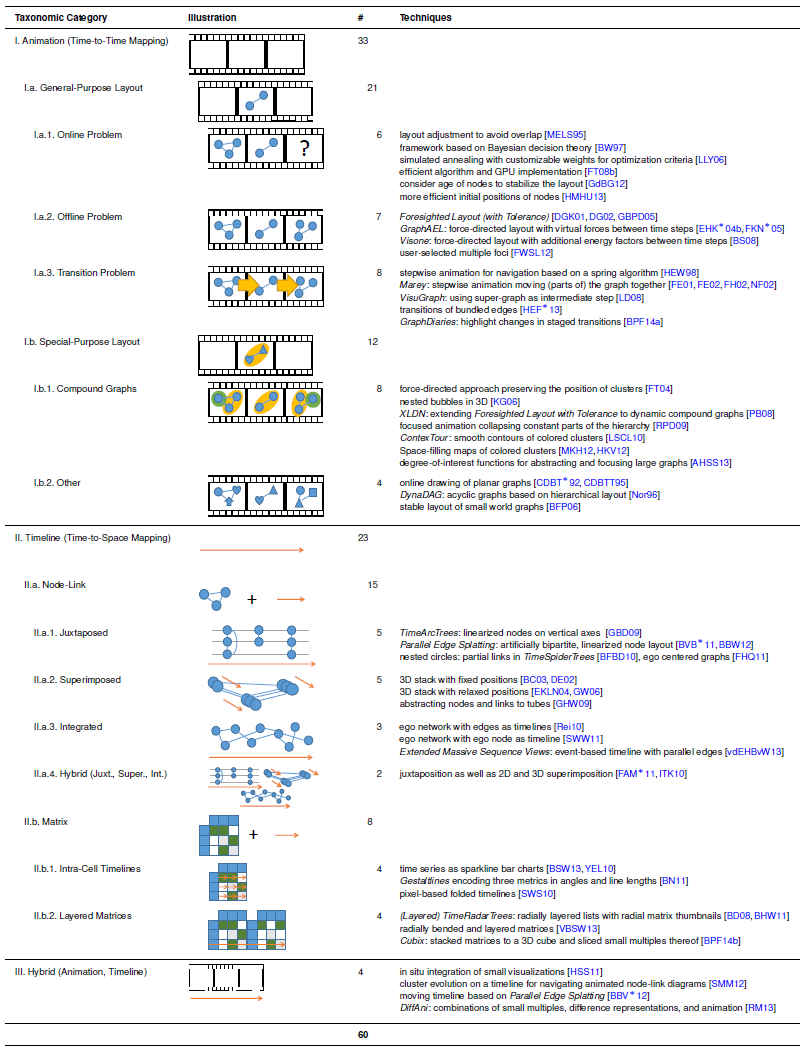
\includegraphics[width=0.5\textwidth]{images/beck2014state.png}
%\caption{Hierarchical taxonomy of dynamic graph visualization courtesy of Beck et al.\ \cite{beck2014state}.} \label{fig: beck2014state}
%\end{center}
%\end{figure}

%\item \textit{Classification Dimensions:}
%\begin{itemize}
%\item[X:] Category, Illustration, No. of Papers, Techniques
%\item[Y:] Categorization: [Time-to-time Mapping, Time-to-space Mapping]
%\item[Y$^1$:] Time-to-time Mapping: [General Purpose Layout: [Online Problem, Offline Problem, Transition Problem],\\ Special-Purpose Layout: [Compound Graphs, Other] ]
%\item[Y$^2$:]Time-to-space Mapping: [Node Link: [Juxtaposed, Superimposed, Integrated, Hybrid],\\ Matrix: [Intra-cell timelines, layered matrices] ]
%\item \textbf{Papers:} 60 Papers cited in Survey \{1992-2015\}\\
%\item{Site:} \url{http://dynamicgraphs.fbeck.com/}
%\end{itemize}

%\item \textit{Unsolved Problems/Future Research:}
Beck et al.\ point out a number of open research areas in the field including the evaluation of dynamic graph visualization techniques, scalability of dynamic graphs, a larger effort in hybrid visualization, extended dimensionality of data, new interaction approaches, and new applications for dynamic graph visualization itself.
%\end{enumerate}

%Title: \textit{The Design Space of Temporal Graph Visualization} by Kerracher et al. \cite{kerracher2014design}
%\begin{enumerate}
%\item \textit{The Concept:}
Kerracher et al.\ present a paper which identifies the design space of temporal graph visualization \cite{kerracher2014design}. They aim to identify this design space, expanding the classification to create an open research area, and raising awareness of the temporal graph visualization field.
%\item \textit{The Scope:}
The design space of temporal graph visualizations is divided into two categories, a graph structural dimension and a temporal dimension, before looking at a combined view. After showing a topology of their survey results, they discuss their findings.

%\item \textit{Classification:}
The design space presented specifies a correlation between specific temporal encodings and specific graph structural encodings. Kerracher et al.\ create a 7x5 matrix yielding a total of 35 different combination of temporal graph visualizations (Figure \ref{fig: kerracher2014design}). Of these 35, 14 are not filled. The design space also color shades  each cell based on the density of papers having this combination. This design space informs the reader that node-links within a sequential view are the most common type of temporal graph visualization.

\begin{figure*}[t]
\begin{center}
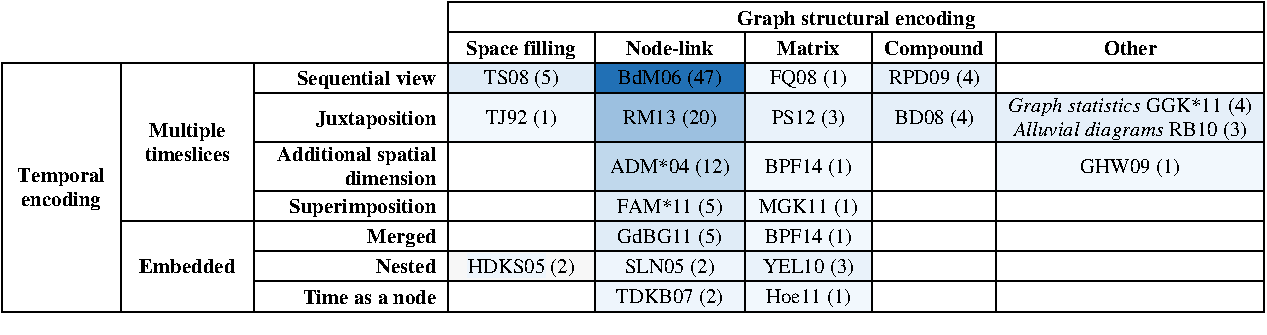
\includegraphics[width=1\textwidth]{images/kerracher2014designFull}
\caption{Design Space for Temporal Graph Visualization. Shading represents the number of papers found per combination (number in brackets). Courtesy of Kerracher et al.\ \cite{kerracher2014design}} \label{fig: kerracher2014design}
\end{center}
\end{figure*}

%\item \textit{Classification Dimensions:}
%\begin{itemize}
%\item[X:] Graph Structured Encoding: [Space Filling, Node-link, Matrix, Compound, Other]
%\item[Y:] Temporal Encoding: [Sequential View, Juxtaposition, Additional spatial dimension, Superimposition, Merged, Nested, Time as a node]
%\item[Z:] Color: Shading represents distribution of papers.
%\item \textbf{Papers:} 128 Papers cited in Survey \{1983-2014\}\\
%\end{itemize}
%
%\item \textit{Unsolved Problems/Future Research:}
Kerracher et al.\ suggest that there could be more research on temporal visualizations using space filling techniques, as well as matrices for dense networks. There are also many unexplored areas found within their design space. An example of this would be a space-filling graph with superimposed time-slices (refer to Figure \ref{fig: kerracher2014design}).
%\end{enumerate}

%Title: \textit{The State of the art in Visualising Group Structures in Graphs} by Vehlow et al. \cite{vehlow2015state}
%\begin{enumerate}
%\item \textit{The Concept:}
\textit{`Graphs or networks are used to model relationships between
objects of any kind'} \cite{vehlow2015state}. Vehlow et al.\ survey the use of these group structures within graph visualization in order to gain a meaningful insight into the underlying data. They provide a classification of techniques used to visualize these group structures.
%\item \textit{The Scope:}
Vehlow et al.\ present an overview of group structures in graphs and their encodings before presenting their classification table. The survey discusses node attributes, juxtaposed visualization, superimposed visualization, and nested visualizations.

%\item \textit{Classification:}
Vehlow et al.\ classify the surveyed papers based on group structure and group visualization. The group structure can be categorized as disjoint flat, overlapping flat, disjoint hierarchy and overlapping hierarchy (the figure is provided in the supplementary material). Of these four, disjoint hierarchy is the most densely populated. Color nodes, glyph nodes, juxtaposition, superimposition, and nested visualizations are identified visualization techniques (see Figure \ref{fig: vehlow2015state1}).

%\begin{figure}[ht]
%\begin{center}
%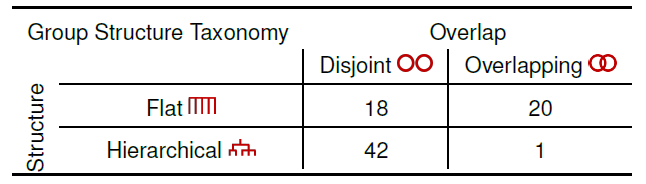
\includegraphics[width=0.48\textwidth]{images/vehlow2015state2.png}
%\caption{Classification of different group structures crourtesy of Vehlow et al.\ \cite{vehlow2015state}. \label{fig: vehlow2015state2}}
%\end{center}
%\end{figure}
\begin{figure}[p]
\begin{center}
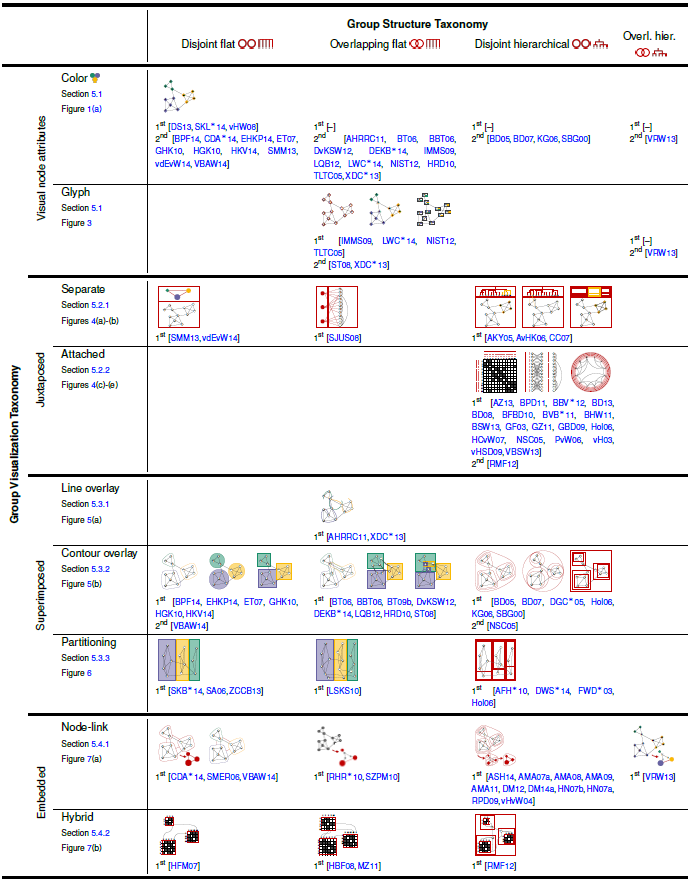
\includegraphics[width=1\textwidth]{images/vehlow2015state1.png}
\caption{Taxonomy table created by Vehlow et al.\ correlating group visualizations and group structures. Courtesy of Vehlow et al.\ \cite{vehlow2015state}} \label{fig: vehlow2015state1}
\end{center}
\end{figure}

%\item \textit{Classification Dimensions:}
%\begin{itemize}
%\item[X:] Group Structure: [Disjoint flat, Overlapping flat, Disjoint Hierarchical, Overlapping Hierarchical]
%\item[Y:] Group Visualization: [Embedded, Superimposed, Juxtaposed, Visual Node Attributes]
%\item \textbf{Papers:} 215 Papers cited in Survey \{1991-2015\}\\
%\end{itemize}

%\item \textit{Unsolved Problems/Future Research:}
Vehlow et al.\ interview 7 domain experts to identify 5 research challenges in the domain. These are time-varying groups and comparison, data complexity, scalability, and the use of interaction techniques such as providing alternative group structures based on users' instructions. The final research challenge identified focus on tasks and evaluation. This involves evaluating group structures based on given tasks in order to analyze the most appropriate group structure to visualize.
%\end{enumerate}

%Title: \textit{A Task Taxonomy for Temporal Graph Visualization} by Kurracher et al. \cite{kerracher2015task}
%\begin{enumerate}
%\item \textit{The Concept:}
Kerracher et al.\ look at the quickly-developing research area of visual representations of temporal graphs. This taxonomy reviews the design space  in a way that enables the reader to review overlapping task categories for the purpose of formalizing graph decisions based on these criteria. \cite{kerracher2015task, kerracher2015visual}.
%\item \textit{The Scope:}
Kerracher et al.\ incorporate the Andrienko Task Framework (ATF) \cite{andrienko2006exploratory}  as the foundation of their classification (the figure is provided in the supplementary material). They analyze the limitations of the framework and propose an extension to consider structural tasks. They then present a summary of tasks primarily for the use of temporal graphs.

%\item \textit{Classification:}
%Their task categorization includes a variation of comparison, relation seeking and lookup tasks, which are combined and reviewed as variants of inherent structural tasks.

Kerracher et al.\ use the Andrienko Task Framework (ATF) \cite{andrienko2006exploratory} to create an indirect classification for their survey. This  task categorization includes lookup tasks, comparison tasks, and relationship seeking tasks. This is combined with a classification of data items (the figure is provided in the supplementary material) discussed in their previous work, \textit{The Design Space of Temporal Graph Visualization} \cite{kerracher2014design}.

%\begin{figure}[ht]
%\begin{center}
%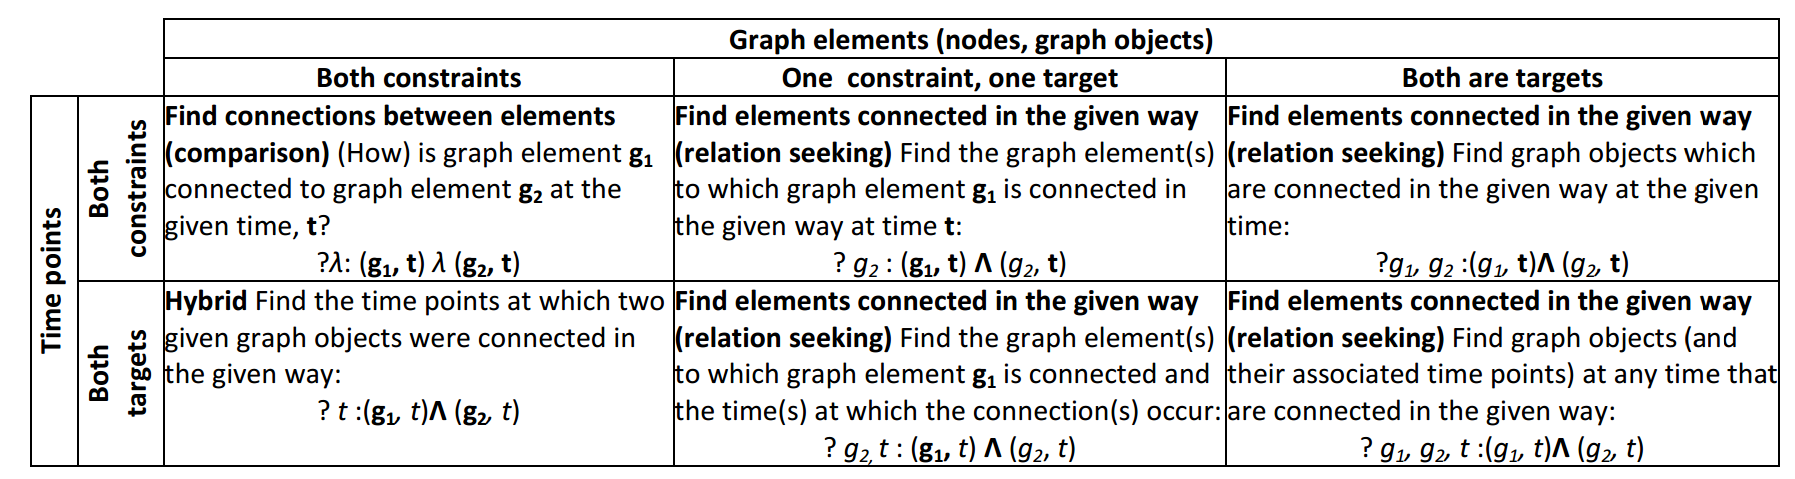
\includegraphics[width=0.5\textwidth]{images/kerracher2015task2.png}
%\caption{Classification of elementary structural task variations. Courtesy of Kerracher et al.\ \cite{kerracher2015task}} \label{fig: kerracher2015visualtask}
%\end{center}
%\end{figure}

%\item \textit{Classification Dimensions:}
%\begin{itemize}
%\item[~]\begin{center} Classifcation Structure: 2D Hierarchical \end{center}
%\item[X:] Graph Elements: [Both Constraints, One Constraint, One Target, Both are Targets]
%\item[Y:] Time Points: [Both Targets, Both Constraints]
%\item \textbf{Site:} n/a \url{}
%\item \textbf{Papers:} 30 Papers cited in Survey \{1983-2014\}\\
%\end{itemize}

%\item \textit{Unsolved Problems/Future Research:}
%Kerracher et al.\ point out a few areas for future research in the field. Using the task taxonomy, a new classification can be made for more than graph areas, such as static graphs, multivariate graphs, and graph comparison. The taxonomy also opens up more research into temporal graphs, with a focus on classification of visualization techniques and mapping tasks to real world scenarios.  These could lead to further research on edges cases or unsupported tasks.

%\end{enumerate}


%Title: \textit{Visual Techniques to Support Exploratory Analysis of Temporal Graph Data} by Kerracher et al. \cite{kerracher2015visual}
%\begin{enumerate}
%\item \textit{The Concept:}
Kerracher et al.\ examine the quickly-developing research area that is visual representation of temporal graphs, with a focus on techniques to support exploratory analysis tasks \cite{kerracher2015visual}.
%\item \textit{The Scope:}
Kerracher et al.\ discuss a task classification which is used to create groups of exploratory tasks based on data attributes. The paper then maps visualization techniques to the quadrant classification as well as the tasks categories and provides examples of the related systems (the figure is provided in the supplementary material).

%\item \textit{Classification:}


%\begin{figure}[ht]
%\begin{center}
%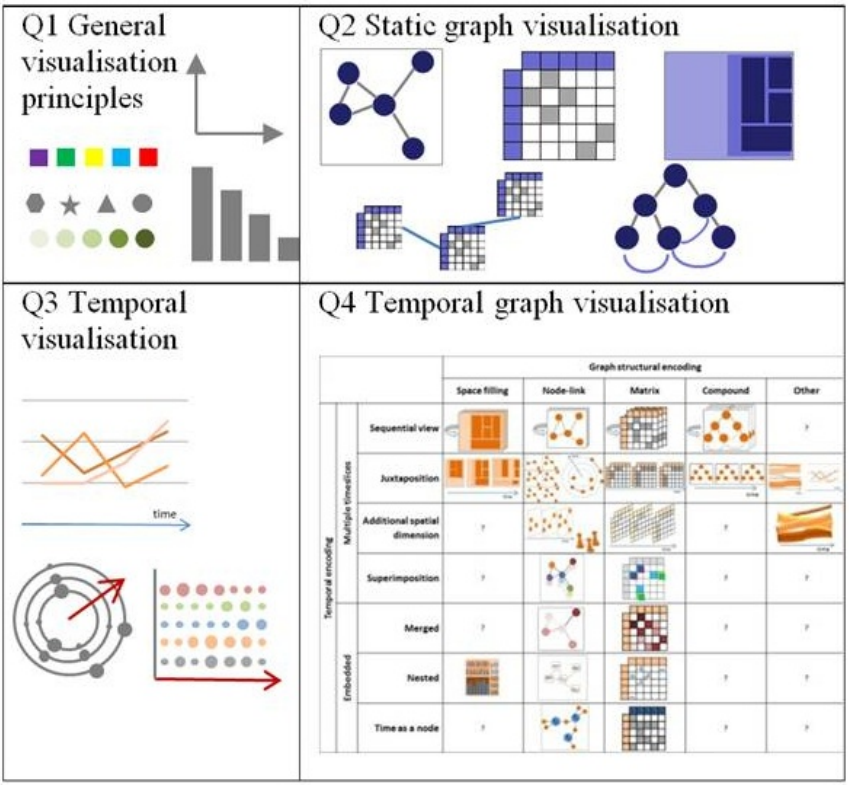
\includegraphics[width=0.47\textwidth]{images/kerracher2015visual.png}
%\caption{Research areas and techniques associated with data items by quadrant. Courtesy of Kerracher et al.\ \cite{kerracher2015visual}} \label{fig: kerracher2015visual}
%\end{center}
%\end{figure}

%\item \textit{Classification Dimensions:}
%\begin{itemize}
%\item[X:] Graph: [Element, Subgraph]
%\item[Y:] Time: [Interval, Point]
%\item \textbf{Site:} n/a \url{}
%\item \textbf{Papers:} 34 Papers cited in Survey \{1990-2014\}\\
%\end{itemize}

Kerracher et al.\ point out a few areas for future research in the field. Using the task taxonomy, a new classification can be made for more than graph areas, such as static graphs, multivariate graphs, and graph comparison. The taxonomy also opens up more research into temporal graphs, with a focus on classification of visualization techniques and mapping tasks to real world scenarios.  These could lead to further research on edges cases or unsupported tasks.

%\item \textit{Unsolved Problems/Future Research:}
They note that more research needs to be aimed at incorporating techniques from a wider range of research areas than the ones typically associated with temporal graph visualization. In particular, techniques used to support the comparisons of data items in temporal graph visualization. 
%\end{enumerate}

\subsubsection{Network Surveys}
This section provides an understanding of the survey landscape for network visualization. Bertin defines a network as the following: `\textit{when the correspondences on a plane can be established among all the elements of the same component, the graphic is a network}' \cite{bertin1983semiology}. This SoS discusses two surveys on this topic which include a task taxonomy with focus on network evolution analysis and a classification of matrix reordering methods for network visualization.

%Title: \textit{A Task Taxonomy for Network Evolution Analysis} by Ahn et al. \cite{ahn2014task}
%\begin{enumerate}
%\item \textit{The Concept:}
Ahn et al.\ provide a literature review with a focus on visualization tasks for network evolution analysis. The paper surveys 53 existing systems and creates a taxonomy with the aim of providing suggestions for designing future visualization tools in the domain \cite{ahn2014task}. This paper could also be categorized in the temporal space of the SoS but is presented here since networks are the primary focus.
%\item \textit{The Scope:}
The paper identifies three aspects of the systems: entities, properties, and temporal features. These aspects are broken down to create the design space for network evolution analysis. The paper uses the design space to analyze task frequency within network evolution analysis and surveys domain experts on their views of the design space. 
The results show 67\% of domain experts rated the design space as very positive (see Figure \ref{fig: ahn2014task}).


%\item \textit{Classification:}
The three aspects of the system identified (entities, properties, and temporal features) are used to create the design space for network evolution analysis. The entities are broken into three subcategories including node/link, groups, and networks. The entity signifies what is being analyzed. Temporal features are displayed on the Y-axis, looking at individual events, shape of changes, and the rate of changes. The properties of the task are displayed inside the table and provide guidance on when a task can be applied, and what information is needed.

\begin{figure}[p]
\begin{center}
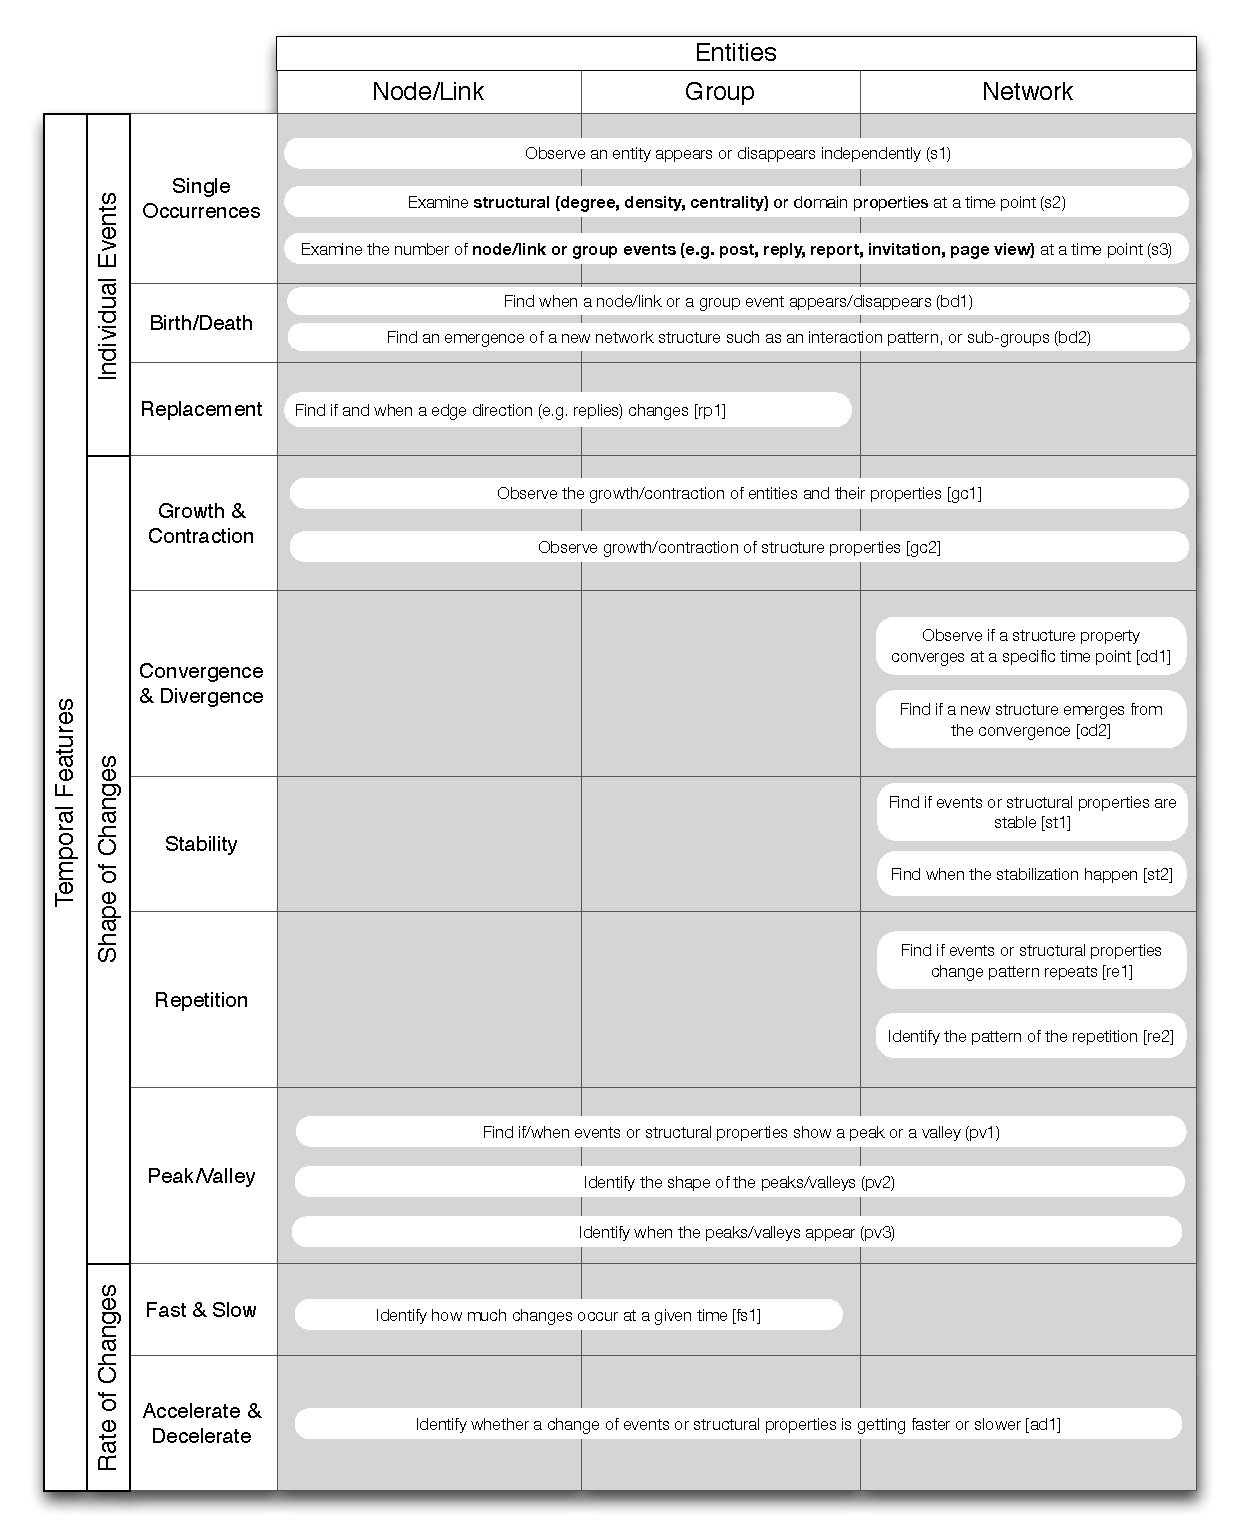
\includegraphics[width=1\textwidth]{images/ahn2014taskFull}
\caption{Design Space of network temporal evolution tasks courtesy of Ahn et al.\ \cite{ahn2014task}} \label{fig: ahn2014task}
\end{center} \vspace{-0.3cm}
\end{figure}

%\item \textit{Classification Dimensions:}
%\begin{itemize}
%\item[~]\begin{center} Classifcation Structure: Hierarchical \end{center}
%\item[L:] Emperical Methods: [Model, Evaluation],\\
%Interactions: [WIMP interactions, Post-WIMP interactions],\\
%Frameworks: [Systems and Frameworks],\\
%Applications: [Graph Visualization, Map Visualization, Multivariate Data Visualization].
%\item \textbf{Site:} n/a \url{}
%\item \textbf{Papers:} 96 Papers cited in Survey \{1986-2013\}\\
%\end{itemize}

%\item \textit{Unsolved Problems/Future Research:}
Future research directions for this field include reviewing the importance of domain properties, additional research on temporal features such as \textit{rate of changes}. Granularity or the scale for analysis had few related papers and is an option for future research. Finally, more research into compound tasks is considered a critical research direction by experts in the field.

%\end{enumerate}

%Title: \textit{Matrix Reordering Methods for Table and Network Visualization} by Behrisch et al.\ \cite{behrisch2016matrix}
%\begin{enumerate}
%\item \textit{The Concept:}
Behrisch et al.\ provide an overview of algorithms used to reorder visual matrices of tabular data. A visual matrix is defined as a visual representation of tabular data used to depict graphs and networks \cite{behrisch2016matrix}. Their survey provides a guide to reordering algorithms in a unified manner to enable a wide audience to understand their differences and subtleties, and provides an overview of how, and when these algorithms are used.
%\item \textit{The Scope:}
Behrisch et al.\ start by providing an introduction to the visual matrix. They discuss the different pattern types which can be used with matrices before deriving their taxonomy. They review some examples of each, before comparing the performance, and how they were tested. The paper finishes by describing directions on algorithm selection. 

%\item \textit{Classification:}
The matrix reordering algorithms are classified into seven families. These families are grouped by the type of algorithm which includes Robinsonian, Spectral, Dimension Reduction, Heuristic Approaches, Graph Theoretic, Bi-clustering, Interactive User-Controlled.

%\begin{figure}[ht]
%\begin{center}
%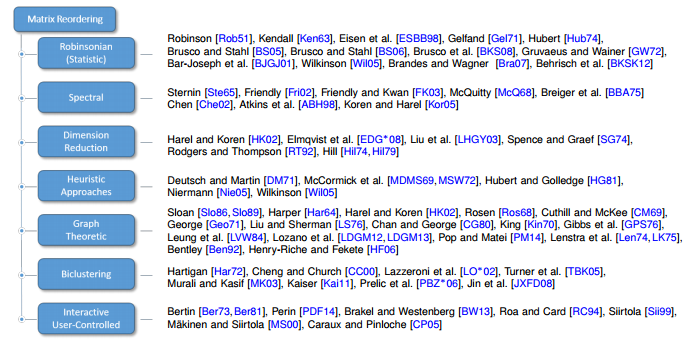
\includegraphics[width=0.5\textwidth]{images/behrisch2016matrix}
%\caption{Taxonomy presented by Behrisch et al.\ classifying different matrices reordering algorithms \cite{behrisch2016matrix} .} \label{fig: behrisch2016matrix}
%\end{center}
%\end{figure}

%\item \textit{Classification Dimensions:}
%\begin{itemize}
%\item[~]\begin{center} List  \end{center}
%\item[L:] Robinsonian (Statistic), Spectral, Dimension Reduction, Heuristic Approaches, Graph Theoretic, Biclustering, Interactive User-Controlled.
%\item \textbf{Site:} \url{http://matrixreordering.dbvis.de}
%\item \textbf{Papers:}  50 Papers cited in Survey \{1992-2014\}\\
%\end{itemize}

%\item \textit{Unsolved Problems/Future Research:}
Some of the open research directions include hybrid solutions to `global vs local' algorithms, and research into similarity, or distance calculation. Frameworks to assess the quality of patterns within matrices and craft objective functions  to optimize algorithms' performance, and human assisted reordering are important.

%\end{enumerate}



\subsection{Geospace + Time}
The section presents at two different visualization types, geospatial visualization and temporal visualization. We place time and geospace together since they are both traditionally dimensional types of data.
\subsubsection{Time Oriented Surveys}
Here we cover surveys with a primary emphasis on time-series data or visualization across multiple time-slices. The SoS summarizes two surveys. The first paper provides a classification for visualization of dynamic data. The second paper provides an understanding of different ways to review slices of data within a Space-Time Cube. 

%Title: \textit{Watch This: A Taxonomy for Dynamic Data Visualization} by Cottam et al.\ \cite{cottam2012watch}.
%\begin{enumerate}
%\item \textit{The Concept:}
Cottam et al.\ review the impact of dynamic data on Information Visualization, and how this data change can influence a visualization's discernability. This is done via the creation of a taxonomy that categorizes dynamic visualization techniques. The paper defines dynamic visualizations as "visualizations that change over time" \cite{cottam2012watch}.

%\item \textit{The Scope:}
Cottam et al.\ present the dimensions of their classification before presenting their technique matrix. Each cell of the technique matrix is reviewed, which gives an understanding of how the axes interact with each other. These are then grouped into higher-level identity groups, which represent how each classification cell would update to a new state. The paper ends by matching techniques to task scenarios.

%\item \textit{Classification:}
The classification has three dimensions. The first dimension envelopes retinal (visual-based) categories, which include: (1) unchanged (immutable) scales, (2) a known scale, (3) extreme bins which categorize catch-all bins such as "100+", and (4) mutable scales which are dynamic scales. The second dimension identifies spatial categories such as fixed spatial dimension, mutable spatial dimension, new spatial elements (create), and create and deleted spatial elements. The third dimension depicts the higher-level identity groups: identity preserving changes, transitional changes, and immediate changes (the figure is provided in the supplementary material).

%\begin{figure}[ht]
%\begin{center}
%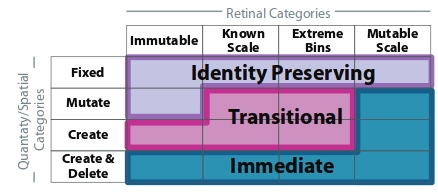
\includegraphics[width=0.49\textwidth]{images/cottam2012watch}
%\caption{A matrix created by Cottam et al.\ to classify different dynamic visualization techniques \cite{cottam2012watch}  .} \label{fig: cottam2012watch}
%\end{center}
%\end{figure}

%\item \textit{Classification Dimensions:}
%\begin{itemize}
%\item[~]\begin{center} Classification Structure: Hierarchical \end{center}
%%\item[List:]
%\item[x:] Retinal Categories: [Immutable, Known Scale, Extreme Bins, Mutable Scale]
%\item[y:] Spatial Categories: [Fixed, Mutate, Create, Create \& Delete]
%\item[3:] Higher-Level Identity Groups: [Identity Preserving, Transitional, Immediate]
%\item \textbf{Url: } n/a \url{}
%\item \textbf{Papers: }49 Papers cited in Survey \{1986-2012\}\\
%
%\end{itemize}

%\item \textit{Unsolved Problems/Future Research:}
Cottam et al.\ consider that the taxonomy could be extended by looking at additional spatial categories, such as "delete but not create." The categories are not distributed evenly, so a study into why is also suggested.
%\end{enumerate}


%Title: \textit{A Review of Temporal Data Visualizations Based on Space-Time Cube Operations} by Bach et al. \cite{bach2014review}
%\begin{enumerate}
%\item \textit{The Concept:}
Bach et al.\ survey a variety of temporal data visualization techniques and discuss how their operations can be used with space-time cubes in order to create a simple  visualization from the 2D+time model. \cite{bach2014review}
%\item \textit{The Scope:}
The paper discusses common static space-time cube operations which includes time-cutting, time flattening, time juxtaposition, space cutting, space flattening, sampling, and 3D rendering. Bach et al.\ then present the taxonomy of space-time cube operations that they have designed before giving the reader a selected sample of multi-operation systems.

%\item \textit{Classification:}
The taxonomy (see Figure \ref{fig: bach2014review}) presents a classification of elementary space-time cube operations such as drilling, cutting and chopping. These are broken down into sub-sections with schematic illustrations in order to enable the user to easily understand what effect the operation has. For example, the flattening section is broken down into planar flattening and non-planar flattening. Planar flattening is broken down into orthogonal flattening and oblique flattening.


\begin{figure}[p]
\begin{center}
\includegraphics[width=1\textwidth]{images/bach2014reviewFull}
\caption{Taxonomy of Space-Time cube operations created by Bach et al.\ \cite{bach2014review} Each operation gives a representation of how the operation may work. Bold font indicates complete operations. Gray shading indicates non-leaf nodes. Image courtesy of Bach et al.\ \cite{bach2014review}} \label{fig: bach2014review}
\end{center}
\end{figure}

%%\item \textit{Classification Dimensions:}
%\begin{itemize}
%\item[X:] Operations, Time, Space
%\item[Y:] Extraction: [Point Extraction, Planar Drilling, Planar Cutting, Non-Planar Cutting, Planar Chopping, Non-Planar Chopping],\\
%Geometry Transformation: [Rigid Transformation, Scaling, Bending, Unfolding],\\
%Content Transformation: [Recoloring, Labeling, Repositioning, Shading, Filtering, Aggregation],\\
%Flattening, Filling.
%\item \textbf{Site:} \url{http://spacetimecubevis.com/}
%\item \textbf{Papers:} 91 Papers cited in Survey \{1970-2013\}\\
%\end{itemize}

%\item \textit{Unsolved Problems/Future Research:}
There are many open research areas that are discussed within the paper. Some of these include interaction techniques such as focus+context to use with different operations, research into operations for extended data dimensions, and understanding which operation is most appropriate for a given task.

%\end{enumerate}

\subsubsection{Geospatial Focused Surveys}
This section focuses on surveys that examine geo-spatial visualization. The section provides an understanding, and classification, of tasks for cartograms, a view of geospatial traffic data, and another review of the use of cartographic visualization in information visualization.

%Title: \textit{A Survey of Traffic Data Visualization} by Chen et al. \cite{chen2015survey}
%\begin{enumerate}
%\item \textit{The Concept:}
Chen et al.\ analyze various ways traffic data can be recorded as well as some different approaches that are brought forward to depict a combination of spatial, temporal, dimensional, and categorical visualization \cite{chen2015survey}.
They systematically review how traffic data is captured. This is divided into three unique categories: Location-Based, which records data as it appears at a fixed point, or sensor range; Activity-Based, which may record data when a specific event is started or finished; Device-Based, recording from a device which records information periodically such as a GPS. Each of these has their own unique benefits and uses. Each data type can be broken down into the four types mentioned previously: spatial; temporal; dimensional; and categorical.
%\item \textit{The Scope:}
Chen et al.\ begin by looking at how the traffic data can be captured and discuss the different ways this data can be processed. The main focus of the survey is how the data is visualized. The paper provides examples of usual design for time, spatial properties, spatio-temporal data, and multi-property data.

%\item \textit{Classification:}
To further improve the taxonomy of traffic data, Chen et al.\ structure the visual design types into the three main goals: Situation-Aware Exploration and Prediction; Pattern Discovery and Clustering; and Visual Monitoring of Traffic Situations. These goals are clearly explained and then presented with relevant examples \cite{chen2015survey}. 

\begin{figure}[t]
\begin{center}
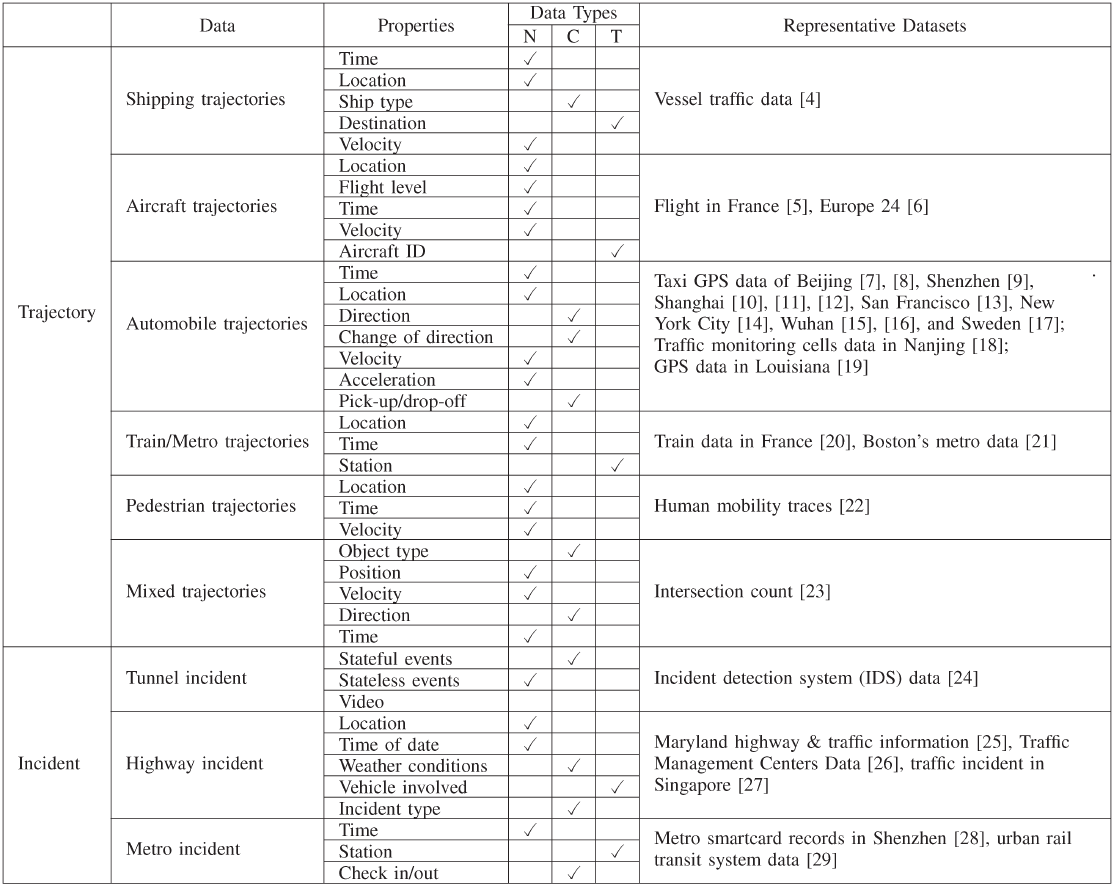
\includegraphics[width=1\textwidth]{images/chen2015survey.png}
\caption{The taxonomy displays different data types with their potential properties. These are then categorized into three data types: Numerical; Categorical; or Textual. Examples of related literature are also given. Courtesy of Chen et al.\ \cite{chen2015survey}}
\end{center}
\end{figure}

%\item \textit{Classification Dimensions: }
%\begin{itemize}
%\item[X:]Tools, Characteristics, Datasets, Platform.
%\item[Y:]Tasks: [Situation-aware exploration and prediction; Pattern discovery and clustering; traffic situations monitoring.]
%\item \textbf{Papers:} 96 Papers cited in Survey \{1991-2014\}\\
%\end{itemize}

%\item \textit{Unsolved Problems}
Chen et al.\ present analysis of situation-aware and immersive environments, as well as the design of huge spatio-temporal analysis of online or streamed data, as open challenges in the field. Visual Analysis of heterogeneous data, social transportation as an example, is another area that requires more focused research.
%\end{enumerate}

%Title: \textit{Task Taxonomy for Cartograms} by Nusrat and Kobourov \cite{nusrat2015task}.
%\begin{enumerate}
%\item \textit{The Concept:}
A cartogram is a type of visualization that aims to combine statistical and geographical information where areas are scaled dependent on statistical proportions. Nusrat and Kobourov study the effectiveness of cartograms as a visualization tool, as well as compare the effectiveness of different cartogram methods. The paper presents a set of cartographic visualization tasks and their application to information visualization \cite{nusrat2015task}.
%\item \textit{The Scope:}
Nusrat and Kobourov begin by providing an overview of cartograms, with related literature for those who want to expand their knowledge of the subject. They then present their design space for cartographic tasks and visual goals for cartogram usage. Both of these are coupled with clear examples of when they could be selected. 

%\item \textit{Classification:}
Nusrat and Kobourov classify tasks by reviewing two hierarchical dimensions, analytic tasks such as identification, location, sorts and clustering (see Figure \ref{fig: nusrat2015task}). The second axis maps visualization goals which includes the goal of the visualization, how a task is carried out, features of the task, and the cardinality. 

\begin{figure}[t]
\begin{center}
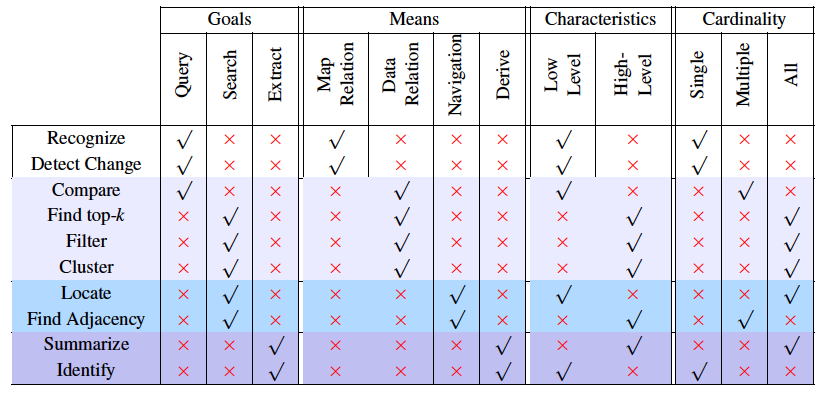
\includegraphics[width=1\textwidth]{images/nusrat2015taskFullp}
\caption{Task taxonomy for cartogram visualization courtesy of Nusrat and Kobourov \cite{nusrat2015task}.} \label{fig: nusrat2015task}
\end{center}
\end{figure}

%\item \textit{Classification Dimensions:}
%\begin{itemize}
%\item[~]\begin{center} Classification Structure: 2D Hierarchical \end{center}
%%\item[List:]
%\item[Y:] Analytic Tasks: [Recognize, Detect Change, Compare, Find top-k, Filter, Cluster, Locate, Find-Adjacency, Summarise, Identify]
%\item[X$^1$:] Goals: [Query, Search, Extract]
%\item[X$^2$:] Means: [Map Relation, Data Relation, Navigation, Derive]
%\item[X$^3$:] Characteristics: [Low-Level, High-Level]
%\item[X$^4$:] Cardinality: [Single, Multiple, All]
%
%
%\item \textbf{Site:} n/a \url{}
%\item \textbf{Papers:} 40 Papers cited in Survey \{1934-2015\}\\
%
%\end{itemize}

%\item \textit{Unsolved Problems/Future Research:}
%n/a
%\end{enumerate}


%Title: \textit{The State of the Art in Cartograms} by Nusrat and Kobourov. \cite{nusrat2016state}
%\begin{enumerate}
%\item \textit{The Concept:}
Nusrat et al.\ follow-up their previous survey with an extended version \cite{nusrat2016state}.
%\item \textit{The Scope:}
They start by presenting a history of cartographic visualization, beginning with their origins in 1870. The paper examines the literature surveys related to cartograms, discussing what is presented in each, before discussing the different design-types of cartographic layouts as well as a task taxonomy extension of `\textit{Task Taxonomy for Cartograms}' by Nusrat and Kobourov \cite{nusrat2015task}, their applications, and their effectiveness.

%\item \textit{Classification:}
They introduce the three major design dimensions of cartographic visualization:
Statistical accuracy, geographical accuracy, and topological accuracy. In addition, cartograms are sub-divided into four different types which include contiguous, non-contiguous, Dorling, and rectangular cartograms.

\begin{figure}[p]
\begin{center}
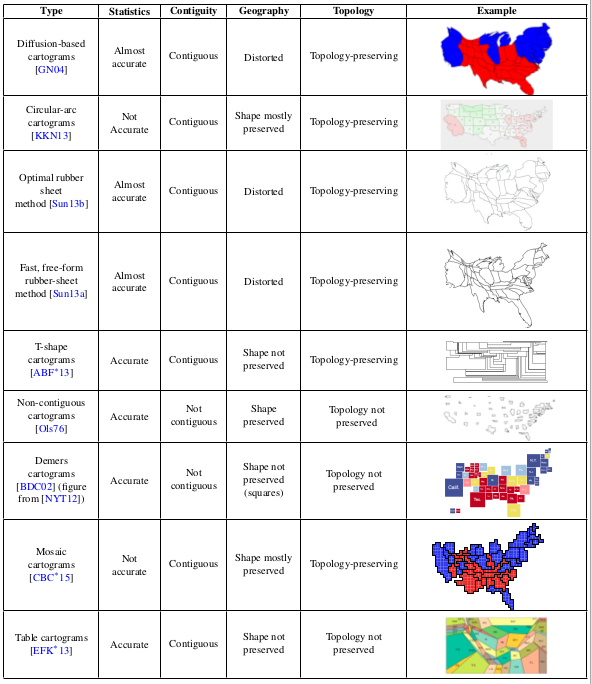
\includegraphics[width=1\textwidth]{images/nusrat2016state.png}
\caption{A 2D systematic overview of different types of cartograms, displayed with their categorizations. Courtesy of Nusrat and Kobourov \cite{nusrat2016state}} \label{fig: nusrat2016state}
\end{center}
\end{figure}

%\item \textit{Classification Dimensions:}
%\begin{itemize}
%\item[X:] Focus: Statistics, Continguity, Geography, Topology, Example
%\item[Y:] Cartogram Type
%\item \textbf{Site:} \url{http://cartogram.cs.arizona.edu/survis-cartogram/}
%\item \textbf{Papers:} 163 Papers cited in Survey \{1932-2016\}\\
%\end{itemize}

%\item \textit{Unsolved Problems/Future Research:}
Nusrat and Kobourov pose a multitude of areas for future cartogram research. Firstly, some of the design dimensions are under-utilized, which could facilitate a paper comparing usage with less used cartographic layouts. Cartograms normally only excel in one of the three design dimension, and a study to mitigate errors in the other two dimensions may allow for a better understanding of cartogram usage. Some other areas of interest are the mapping of multivariate data, memorability and recall within cartograms, uncertainty within cartograms, and 3D cartographic visualization.

%\end{enumerate}

\subsection{Coordinated Multiple View (CMV) Surveys }
Coordinated Multiple Views (CMVs) surveys focus on literature that examines the coordination or linkage between multiple views. This section summarizes two papers related to the subject. The first reviews the use of composite visualization and the second provides an understanding of multi-faceted graph visualization.

%Title: \textit{Exploring the Design Space of Composite Visualization} by Javed and Elmqvist. \cite{javed2012exploring}.
%\begin{enumerate}
%\item \textit{The Concept:}
Javed and Elmqvist examine different Composite Visualization Views (CVVs), which are defined as \textit{"a visual composition of two or more visual structures in the same view,"} and present their CVV design patterns created via a literature survey \cite{javed2012exploring}.
%\item \textit{The Scope:}
They start by discussing different CVVs, including their design patterns  and existing formalisms. This is followed with an in-depth look at the different types of views (juxtaposed, integrated, superimposed, etc), with examples of each. They then present their design space and guidelines, as well as their 1-N classification table.

%\item \textit{Classification:}
The authors look at different techniques and how the visualization's relations are classified. The grouping looks at the result of merging two visual designs, the composite relation (juxtaposed, integrated, superimposed, overloaded, nested), as well as what data-relation is created (item-item, item-group, etc).

\begin{figure}[t]
\begin{center}
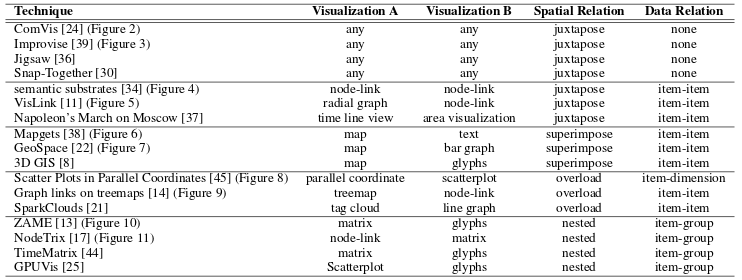
\includegraphics[width=1\textwidth]{images/javed2012exploring}
\caption{ Classification of common composite visualization techniques \cite{javed2012exploring} .} \label{fig: javed2012exploring}
\end{center}
\end{figure}

%\item \textit{Classification Dimensions:}
%\begin{itemize}
%\item[~]\begin{center} Classification Structure: 2D \end{center}
%
%\item[X$^1$:] Visualization A
%\item[X$^2$:] Visualization B
%\item[X$^3$:] Spatial Relation
%\item[X$^4$:] Data Relation
%\item[Y:] Technique
%
%\item \textbf{Site:} n/a \url{}
%\item \textbf{Papers:} 45 Papers cited in Survey \{1885-2013\}\\
%
%\end{itemize}

%\item \textit{Unsolved Problems/Future Research:}
Javed and Elmqvist suggest their design patterns are limited to literature reviewed and therefore work can be invested into extending their framework. The design pattern is also limited to only spatial relation and does not look at other composite visualization views, such as interaction or animation.
%\end{enumerate}

%Title: \textit{A Survey of Multi-faceted Graph Visualization} by Hadlak et al. \cite{hadlak2015survey}
%\begin{enumerate}
%\item \textit{The Concept:}
Many surveys focus on only a single additional facet in order to classify graphing techniques. Hadlek et al.\ aim to build on existing surveys in order to create a more in-depth observation of four common facets: partitions, attributes, time, and space. Each of these characteristics are discussed based on their relationship as well as examples of how these graphs can be represented depending on the hierarchy.
%\item \textit{The Scope:}
Hadlek et al.\ focus on an output oriented perspective, and optimize facet selection by focusing on their composition. These compositions are given a representative visualization (seen in Figure \ref{fig: hadlak2015survey}) to discuss in detail in the content of the survey. Hadlek et al.\ analyse visual design of the graph structure with a single additional facet and graph structure with multiple additional facets. These are sub-divided for each common facet. This is followed by analyzing multiple instances of graph facets.

%\item \textit{Classification:}
Each graph structure is split into five combinations. Whilst looking at the spatial composition, an example is given for structure as the base representation, partitions as the base representation, or a balanced representation. A temporal composition has an example for either structure as the base representation or partitions as the base representation.

\begin{figure}[t]
\begin{center}
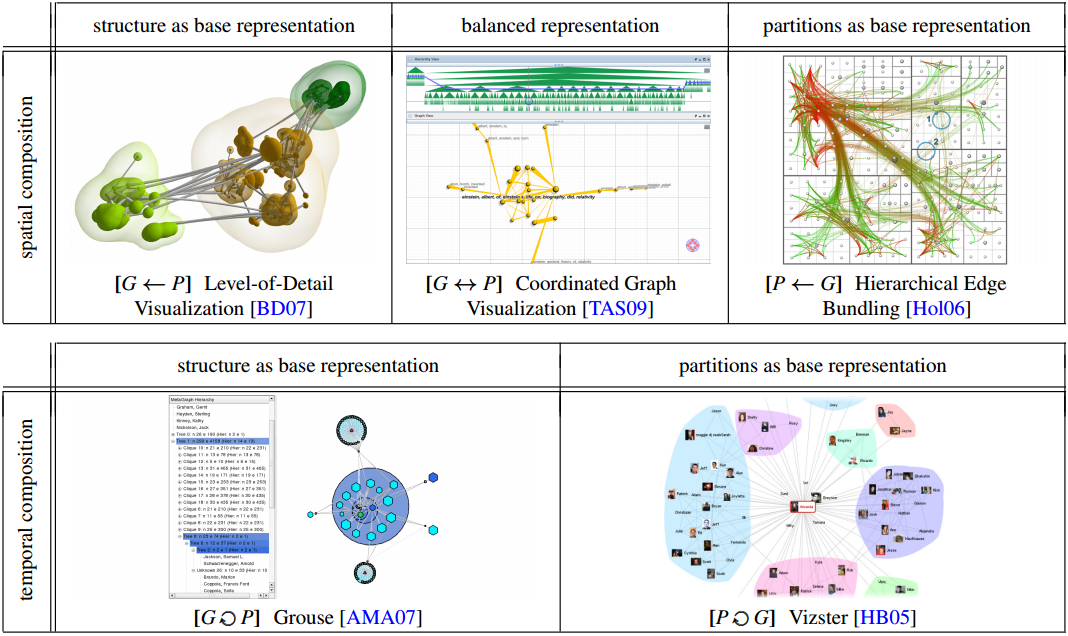
\includegraphics[width=0.8\textwidth]{images/hadlak2015survey.png}
\caption{Examples of multiple facet representations within visualization. Courtesy of Hadlak et al.\ \cite{hadlak2015survey}} \label{fig: hadlak2015survey}
\end{center}\vspace{-0.5cm}
\end{figure}

%\item \textit{Classification Dimensions:}
%\begin{itemize}
%\item[X:] Representation: [Structure as base, Balanced, Time as Base]
%\item[Y:] Compisition: [Spatial, Temporal]
%\item \textbf{Papers:} 133 Papers cited in Survey \{1990-2015\}\\
%
%\end{itemize}

%\item \textit{Unsolved Problems/Future Research:}
The paper notes the exploration of geo-spatial graph visualization, by reviewing output or task taxonomy, has yet to be published. Hadlek et al.\ also point out that some of the facets discussed had very sparse usage such as temporal compositions. Finally, only four facets were examined but there are many other extensions such as provenance, uncertainty, heterogeneity, or text/annotations that have little-or-no exposure which could be a new thread of research to investigate.
%\end{enumerate}

\subsection{Real-World and Applications}
Many literature surveys focus on real-world scenarios and applications. This area covers a wide range of surveys including finance, health-care, security, systems, software visualization, and visualization frameworks.
\subsubsection{Finance Focused Surveys}
This section has a focus on survey papers related to finance visualization. The survey summarizes one paper focused on different sources of financial data and how they are visualized.

%Title: \textit{A Survey on Visual Analysis Approaches for Financial Data} by Ko et al.\ \cite{ko2016survey}
%\begin{enumerate}
%\item \textit{The Concept:}
Ko et al.\ perform and present a study of visualization and visual analytics of financial data. Economy is an important field for any business which has led to financial data being a popular topic for visualization in industries. They aim to utilize existing papers in order to help researchers design better systems and understand new research fields within the area \cite{ko2016survey}.
%\item \textit{The Scope:}
After discussing the survey scope, Ko et al.\ explore the types of data analyzed and some data sources for each. Some examples of this include stock data, transaction data, and fund data. The paper derives a classification of techniques and provides examples of these uses before examining the interaction methods and evaluation methods. This is followed by an evaluation of the papers.

%\item \textit{Classification:}
Ko et al.\ examine multiple ways to classify the gathered information. The first classification tests the type of data used by each paper, which indicates a heavy focus on stock data. The second classification discusses papers based on automated techniques, such as K-means. The third looks at visualization techniques, based on Keim's technique taxonomy \cite{keim2002information} (see Figure \ref{fig: ko2016survey}). The fourth categorization considers interaction methods and the final organization examines evaluation methods.

\begin{figure*}[t]
\begin{center}
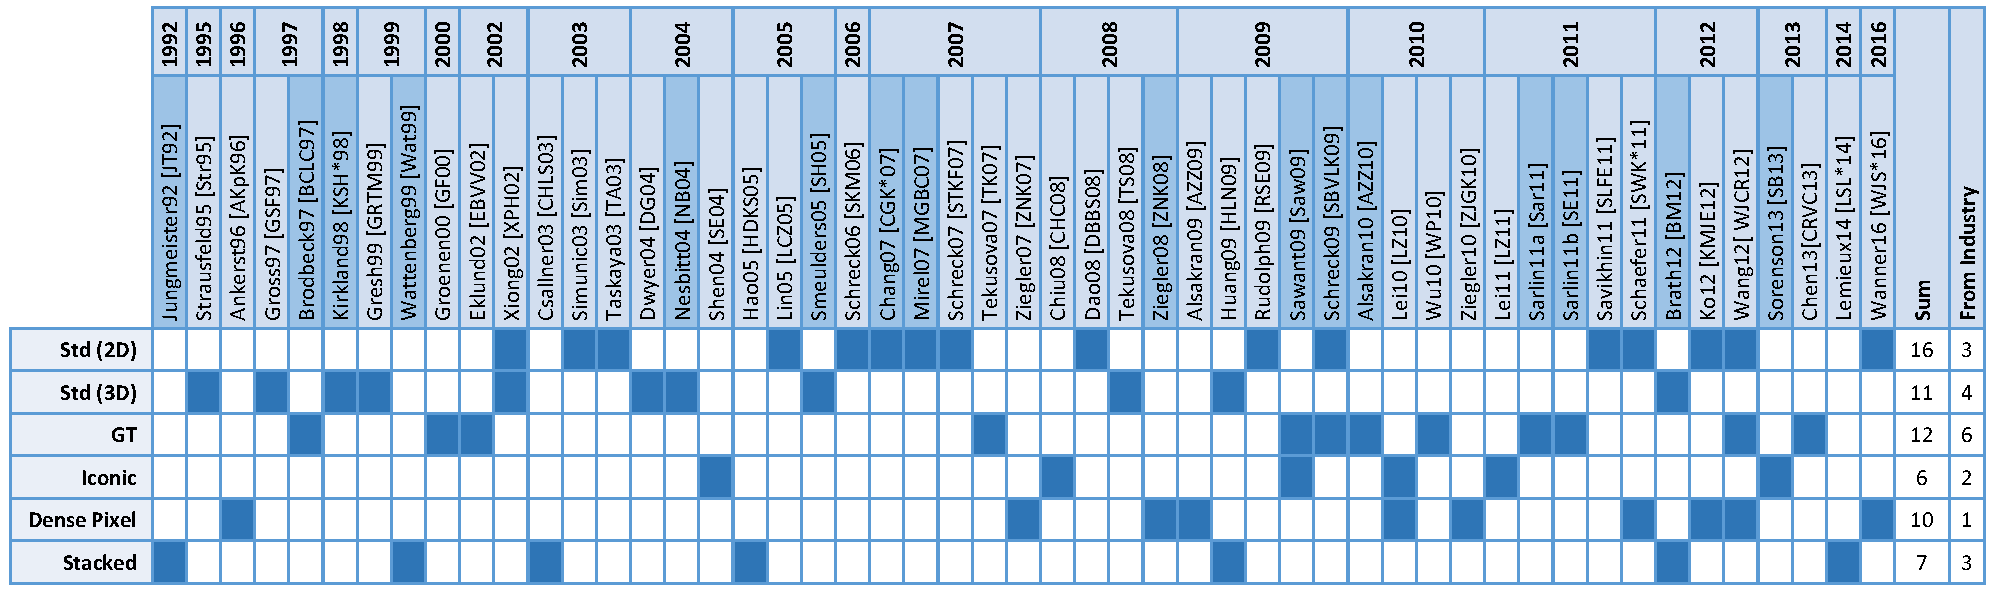
\includegraphics[width=1\textwidth]{images/ko2016surveyFull}
\caption{Ko et al.'s Categorization of surveyed papers via Keim's visualization techniques taxonomy \cite{ko2016survey,keim2002information} .} \label{fig: ko2016survey}
\end{center}
\end{figure*}

%\item \textit{Classification Dimensions:}
%\begin{itemize}
%\item[~]\begin{center} Classification Structure: 2D (x5) \end{center}
%%\item[List:]
%\item[X:] Paper
%\item[Y$^1$:] Data Sources: [Stock, Fund, Econ. Indi., Trans, Risk, Company Info]
%\item[Y$^2$:] Automated Techniques: [K-means, SOM, MDS, PCA, Sampling, Moving Avg., Regression, Decision Tree, Specific Models]
%\item[Y$^3$:] Visualization Techniques: [Std (2D), Std (3D), GT, Iconic, Dense Pixel, Stacked]
%\item[Y$^4$:] Interaction Methods: [Select, Explore, Reconfigure, Encode, Abstract, Filter, Connect]
%\item[Y$^5$:] Evaluation Methods: [Use Case, Case Study, User Feedback, User Study, Performance]
%
%\item \textbf{Site:} n/a \url{}
%\item \textbf{Papers:} 50 Papers cited in Survey \{1992-2014\}\\
%\footnotesize * literal count of cited papers and not papers surveyed.\\
%\end{itemize}

%\item \textit{Unsolved Problems/Future Research:}
They propose that there are nine more business domains which could have their visual analytics reviewed such as economic analysis, financial risk management, and portfolio management. They also discuss the lack of research into company performance with financial data and suggest this as an open field. An important area for research is with automated visualization techniques, which industry experts believe are important to facilitate a richer depth of information. The final point they discuss is the use of heterogeneous data to enable improved prediction models.

%\end{enumerate}
\subsubsection{Security-based Literature Surveys}
This section includes survey papers that present security systems. One features a focus on visualization systems for network security and  another on malware analysis.

%Title: \textit{A Survey of Visualization Systems For Network Security} by Shiravi et al.\ \cite{shiravi2012survey}.
%\begin{enumerate}
%\item \textit{The Concept:}
Shiravi et al.\  provide a comprehensive overview of network security visualization and present data sources for each. The paper also provides a taxonomy that includes literature across five use-cases \cite{shiravi2012survey}.
%\item \textit{The Scope:}
They present a table that provides potential data sources for security visualization before giving an in-depth view of five use-cases for reviewing network security and their related papers. The use-cases are host/server monitoring, internal/external monitoring, port activity, attack patterns, and routing behavior.

%\item \textit{Classification:}
The taxonomy takes the form of a 2D table, sub-divided into five sections representing the five use-cases. The taxonomy reviews the type of visualization techniques and data source of each research paper. It also includes the number of citations a paper has to emphasize systems that have more references, as well as signifying whether the system is available online (the figure is provided in the supplementary material).

\begin{figure}[p]
\begin{center}
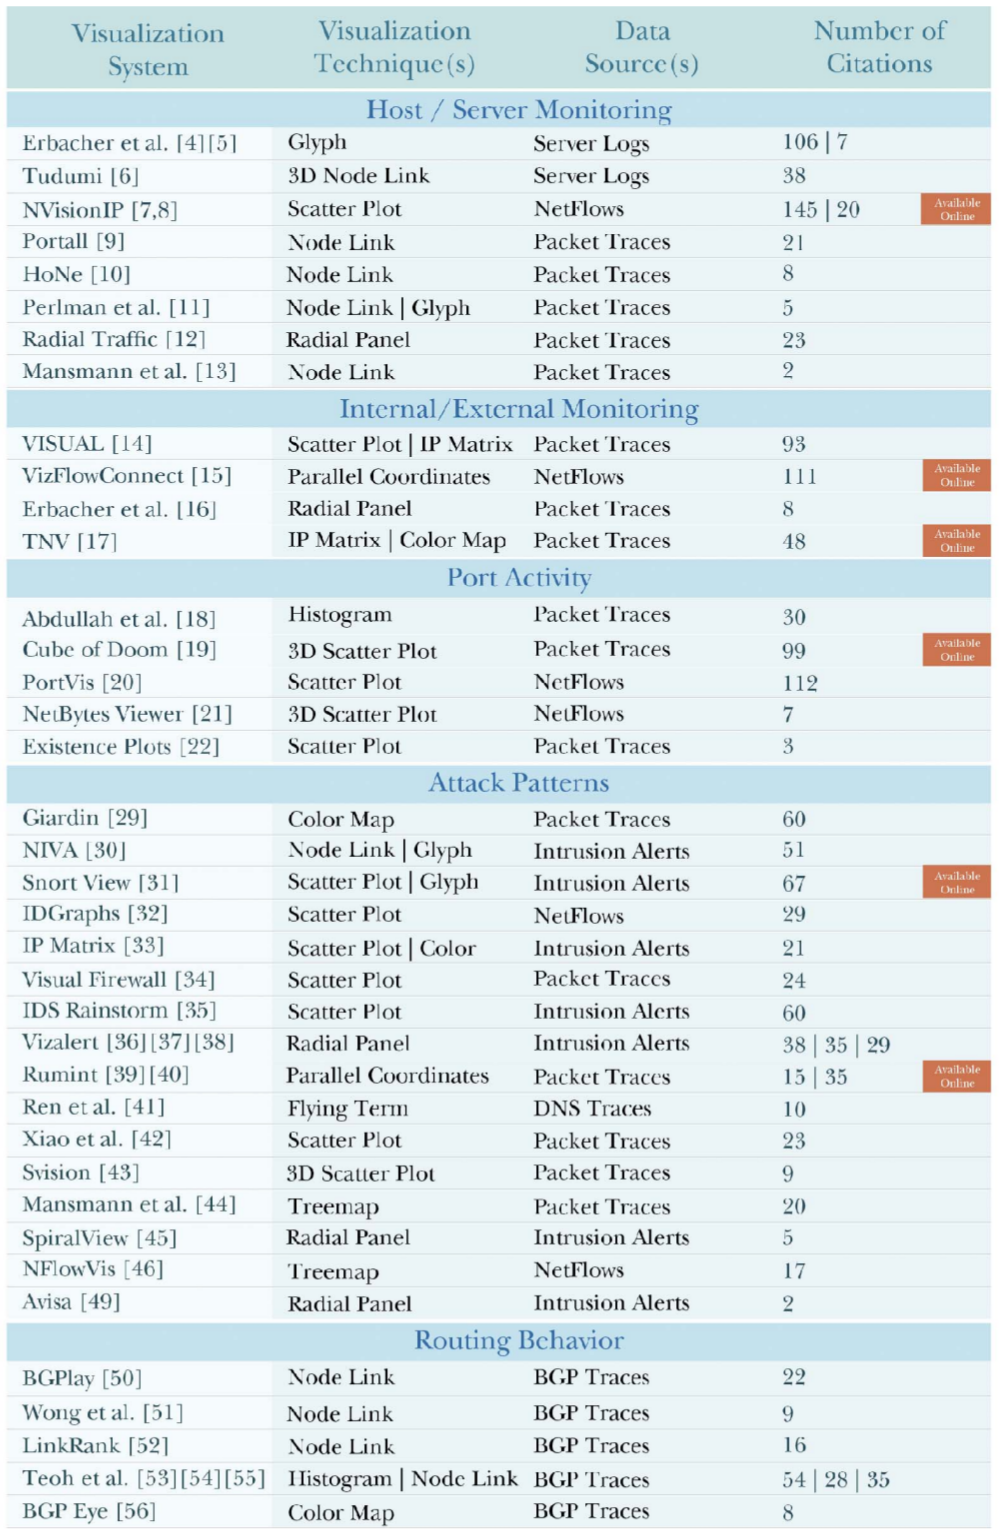
\includegraphics[width=0.8\textwidth]{images/shiravi2012survey}
\caption{Taxonomy of Security Visualization Systems, divided into different use-cases. Created by Shiravi et al.\ \cite{shiravi2012survey} .} \label{fig: shiravi2012survey}
\end{center}
\end{figure}

%\item \textit{Classification Dimensions:}
%\begin{itemize}
%\item[~]\begin{center} Classification Structure: 3D Hierarchical \end{center}
%%\item[List:]
%\item[X$^1$:] Visualization Technique
%\item[X$^2$:] Data Source
%\item[X$^3$:] Number of Citations
%\item[Y:] Visualization System
%\item[Z:] Online Availability
%
%\item \textbf{Site:} n/a \url{}
%\item \textbf{Papers:} 90 Papers cited in Survey \{1995-2011\}\\
%
%\end{itemize}

%\item \textit{Unsolved Problems/Future Research:}
Shiravi et al.\ present future research topics including situation awareness in presenting information, user experience evaluation, scalablity, occlusion in network security, privacy preservation and   novel ways to provide 3D imagery of the data.

%\end{enumerate}

%Title: \textit{A Survey of Visualization Systems for Malware Analysis} by Wagner et al. \cite{wagner2015survey}
%\begin{enumerate}
%\item \textit{The Concept:}
Wagner et al.\ present a systematic overview and classification of malware visualization systems used for visual analysis. The field is gaining more and more interest due to the increasing threat of malware attacks on user systems. Malware is defined as \textit{"any software that does something that causes harm to a user, computer or network"} \cite{wagner2015survey}.
%\item \textit{The Scope:}
They focus on malware systems for visual analysis. They first provide tools, discussed as \textit{data providers}, and provide a comparison of their usage. They present their malware visualization taxonomy and categorize each data provider in a number of different classification groups.

%\item \textit{Classification:}
Wagner et al.\  create three categories for malware visualization systems: (1) Individual malware analysis which enables the system to look at a single malware sample and learn about its individual behavior. (2) Malware comparison which facilitates comparison of a range of malware for viewing. (3) Malware summarisation that outlines the behavior of different malware samples (see Figure \ref{fig: wagner}).

\begin{figure*}[t]
\begin{center}
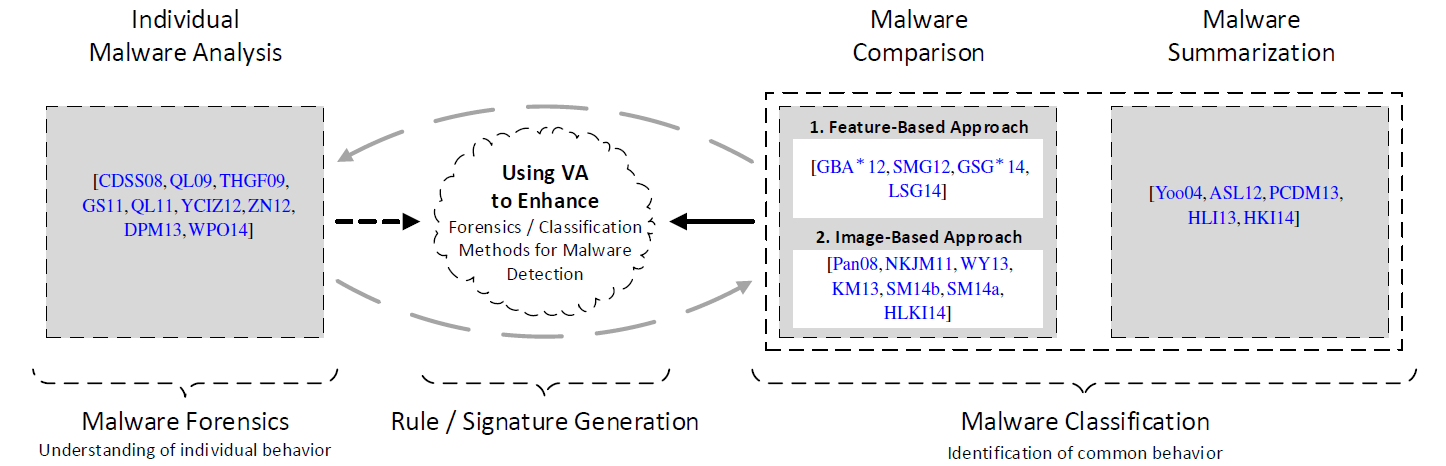
\includegraphics[width=1\textwidth]{images/wagner2015survey.png}
\caption{The 1D malware visualization taxonomy courtesy of Wagner et al.\ \cite{wagner2015survey}} \label{fig: wagner}
\end{center}
\end{figure*}

%\item \textit{Classification Dimensions:}
%\begin{itemize}
%\item[X:] Malware Analysis Tool
%\item[Y:] Base Data, Data Format, Visualization Techniques, Mapping and Representation Space, Temporal Aspects, Interactivity, Tasks.
%\item \textbf{Papers:} 91 Papers cited in Survey \{1974-2015\}\\
%\end{itemize}

%\item \textit{Unsolved Problems/Future Research:}
They find that malware visualization is cleanly partitioned between each classification category and believe more work needs to be done in creating a connection between  categories. Using different systems could cause unnecessary overlap for users which could be minimized with a system that could move through this categorization. Some other challenges in the field include the integration of more data sources, a stronger understanding of the requirements for malware visualization, enabling expert analysis and externalization, and an increased focus on the relation between analysis and visualization for malware.

%\end{enumerate}
\subsubsection{Systems-based Surveys}
This section focuses on Surveys that have an emphasis on classifying systems. We summarize one survey paper in this section which looks at performance visualization of large-scale systems.


%Title: \textit{Performance Visualization for Large-scale Computing Systems} by Gao et al.\ \cite{gao2011performance}
%\begin{enumerate}
%\item \textit{The Concept:}
Gao et al.\ present a review on papers designated for researching performance visualization on large-scale systems. Gao et al.\ define performance visualization as \textit{`the use of graphical display techniques for the visual analysis of performance data'}\cite{gao2011performance}. The paper aims to shed light on open research areas, and increased discussion on the design of visual tools for these systems. 
%\item \textit{The Scope:}
The paper provides a brief background of performance visualization and how it functions.

%\item \textit{Classification:}
Gao et al.\ classify performance visualization techniques using four main categories. Simple visual structures which include statistical charts with one or two variables, composed visual structures that include a combination of simple chart views, interactive visual structures featuring structures that provide a variety of user interactions, and focus+context which refers to visualizations with mapping that is automatically modified without the need of user interaction (the figure is provided in the supplementary material).


\begin{figure}[t]
\begin{center}
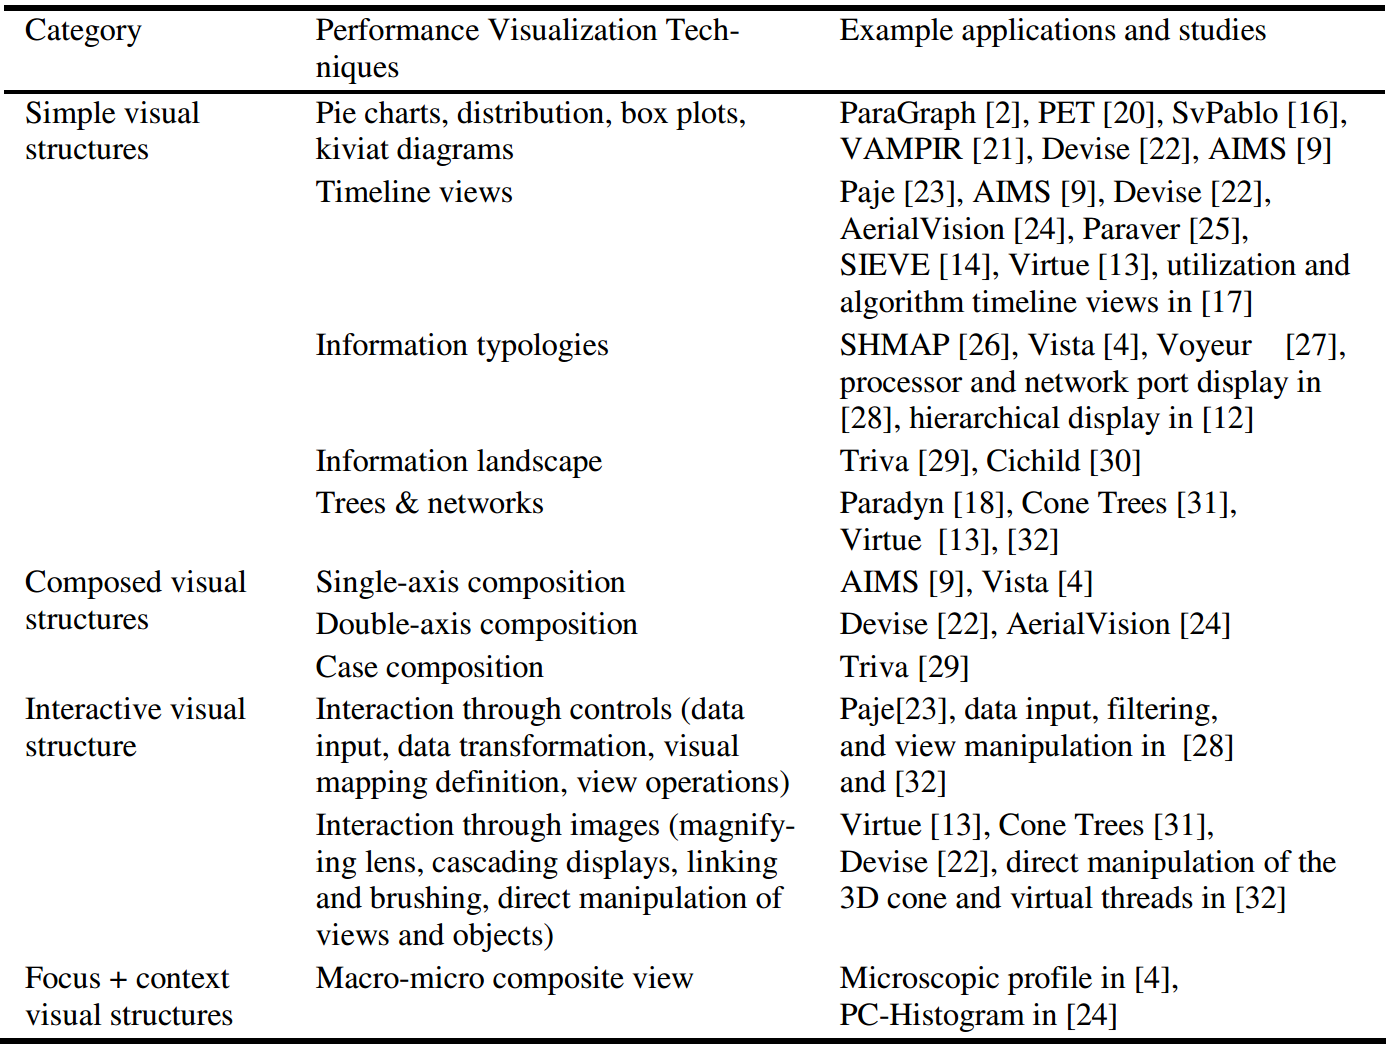
\includegraphics[width=1\textwidth]{images/gao2011performance}
\caption{A classification of performance visualization techniques courtesy of Gao et al.\ \cite{gao2011performance}.} \label{fig: gao2011performance}
\end{center}
\end{figure}

%\item \textit{Classification Dimensions:}
%\begin{itemize}
%\item[~]\begin{center} Classifcation Structure: Hierarchical \end{center}
%\item[L:]Simple Visual Structures: ["Pie Charts, Distribution, Box Plots, Kiviat Diagrams", "Timeline Views", "Information Typologies", "Information Landscape Trees \& Networks"],\\
%Composed Visual Structures: ["Single-Axis Composition", "Double-Axis Composition", "Case Composition"],\\
%Interactive Visual Structure: ["Interaction through controls", "Interaction through image"]\\
%Focus+Context Visual Structures: ["Macro-micro composite view"].
%
%
%\item \textbf{Site:}  n/a \url{}
%\item \textbf{Papers:} 21 Papers cited in Survey \{1923-1998\}\\
%\end{itemize}

%\item \textit{Unsolved Problems/Future Research:}
Some future work areas presented by Gao et al.\ include scalability, user studies, and the synthesis of high-level context with low-level detail.

%\end{enumerate}
\subsubsection{Software Visualization Surveys}
Software Visualization papers focus on visualizing aspects of software creation. Diehl defines the topic as follows:\textit{`Software visualization encompasses the development and evaluation of methods for graphically representing different aspects of software, including its structure, its execution, and its evolution'} \cite{diehl2007software}. The SoS summarizes one recent survey paper in this section that focuses on the static aspects of software visualization.

%Title: \textit{Visualization of the Static Aspects of Software: A Survey} by Caserta and Zendra \cite{caserta2011visualization}.
%\begin{enumerate}
%\item \textit{The Concept:}
Caserta and Zendra categorize visualization techniques that represent the static aspects of software and it's evolution. The paper defines visualization of the static aspects of software as `\textit{visualizing software as it is coded, and dealing with information that is valid for all possible executions of the software}' \cite{caserta2011visualization}. Evolution of software adds a temporal dimension to the visualization of the static aspects of software.
%\item \textit{The Scope:}
The paper provides a guide to papers that feature code-line-centered visualization, class-centered visualization, architecture visualization, and the visualization of software evolution. They provide examples of different types of visual design for each and how they may be applied.

%\item \textit{Classification:}
The hierarchical, 1-N, classification presents the representation and visualization techniques used for each paper, and shows how they fit into their taxonomy (see Figure \ref{fig: caserta2011visualization}).

\begin{figure}[t]
\begin{center}
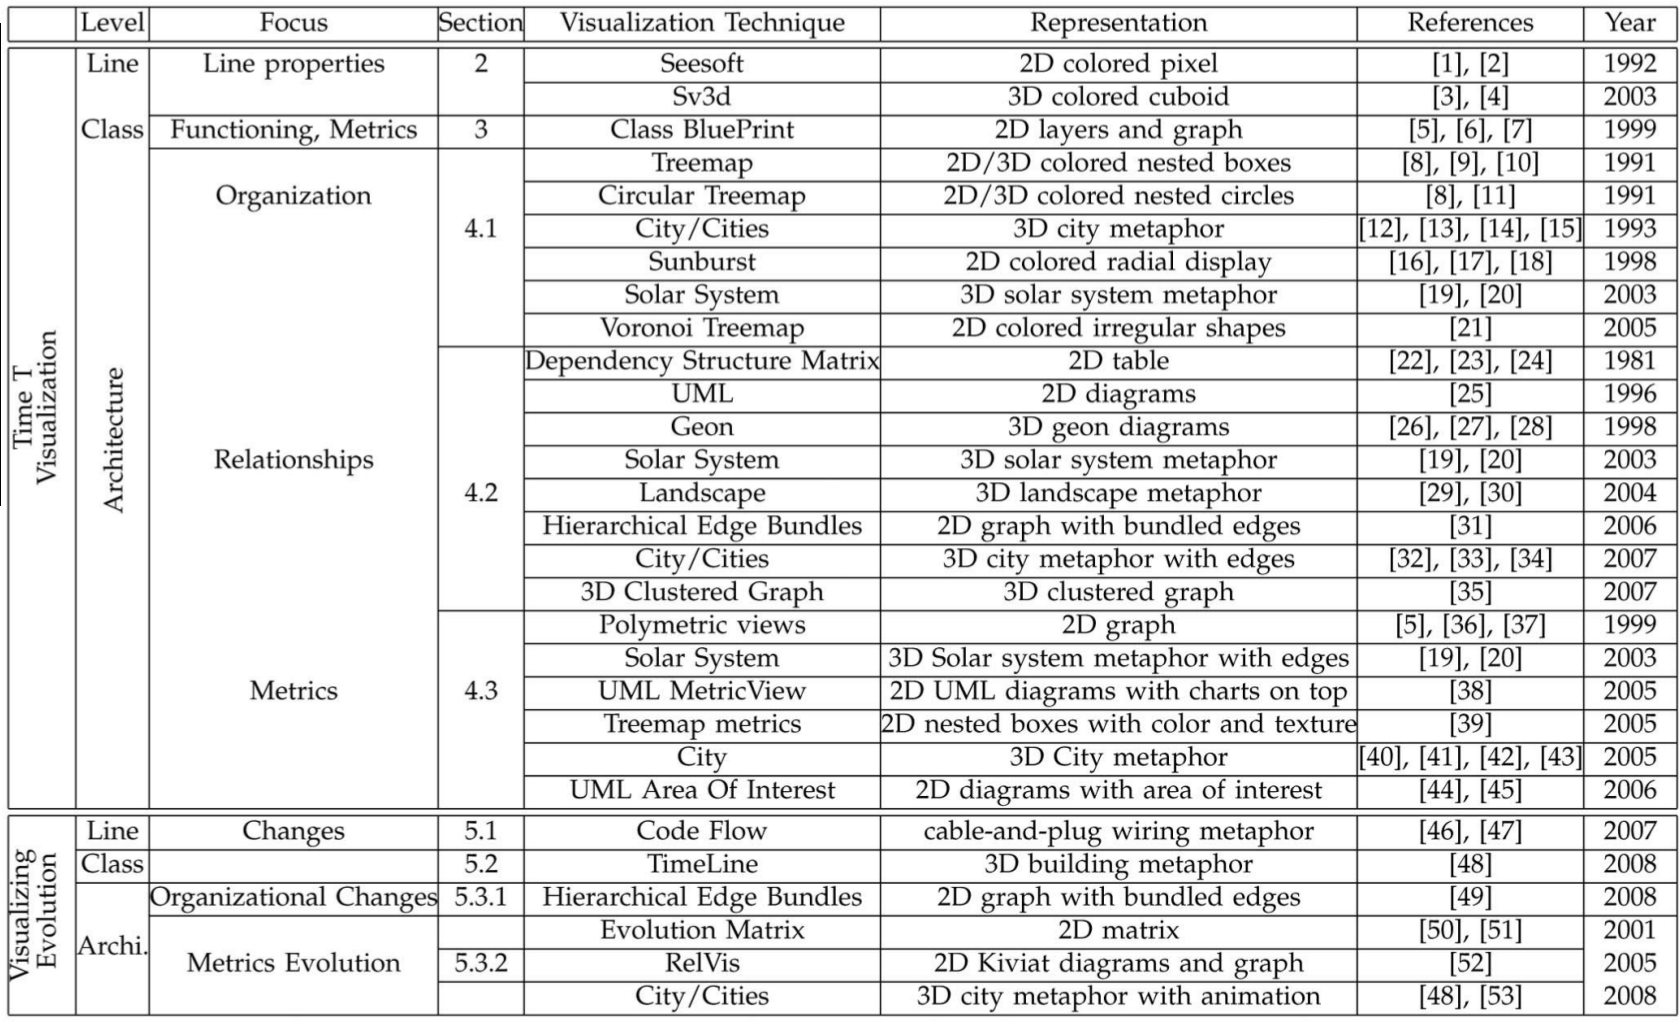
\includegraphics[width=1\textwidth]{images/caserta2011visualization}
\caption{Caserta and Zendra present a table that classifies methods that visualise the static aspects of software and the associated literature \cite{caserta2011visualization} .} \label{fig: caserta2011visualization}
\end{center}
\end{figure}

%\item \textit{Classification Dimensions:}
%\begin{itemize}
%\item[~]\begin{center} Classification Structure: 2D Hierarchical \end{center}
%%\item[List:]
%\item[Z$^1$:] Aspects of Software Visualization: [Static Aspects, Static Aspects + Time]
%\item[X$^2$:] Level: [Code-line-centered, Class-Centered, Architecture]
%\item[X$^3$:] Focus: [Line Properties, Functioning/Metrics, Organisation, Relationships, Metrics, Changes, Orginizational Changes, Metrics Evolution]
%\item[X$^4$:] Visualization Technique
%\item[X$^5$:] Representation
%
%
%\item \textbf{Site:} n/a \url{}
%\item \textbf{Papers:} 192 Papers cited in Survey \{1979-2011\}\\
%
%\end{itemize}

%\item \textit{Unsolved Problems/Future Research:}
Caserta and Zendra propose that it would be beneficial to invest research into usability evaluation to find the most effective ways to visualize the static aspects of software. There is also limited research in navigation and interaction for 3D visualization within the field.

%\end{enumerate}

\subsubsection{Surveys of Frameworks}
This section examines the review of frameworks, which is defined as \textit{`a basic structure underlying a concept'} \cite{frameworkdictionary}. The section covers two surveys: the first presents a design framework survey for bi-cluster visualizations and the second presents a framework for emphasis in visualizations.

%Title: \textit{A Five-Level Design Framework for Bicluster Visualizations} by Sun et al. \cite{sun2014five}
%\begin{enumerate}
%\item \textit{The Concept:}
Sun et al.\ provide a survey focused on bi-cluster visualization, design considerations, and applications. Bi-clusters \textit{"provide a rich high-level abstraction that represents coordinated relationships between groups of entities of different types"} \cite{sun2014five}. The advantages and disadvantages are compared, and a five-level relationship is presented to assist in design options that support user-tasks.
%\item \textit{The Scope:}
The paper describes the concept of bi-clustering and the five relationship levels of the bi-cluster visualization design framework. These include: entity level (single entity relationships), group level (entity group relationships), bi-cluster level (coordinated relationships), chain level (chained coordinated relationships), and the schema level (schema level relationships). The paper also examines four levels of interaction design: readability, navigation, parameter, and object level.

%\item \textit{Classification:}
Sun et al.\ provide a summary of the five-level design framework for bi-cluster visualization. This incorporates the interaction design level, major tasks, design choice, and trade-offs.

\begin{figure}[t]
\begin{center}
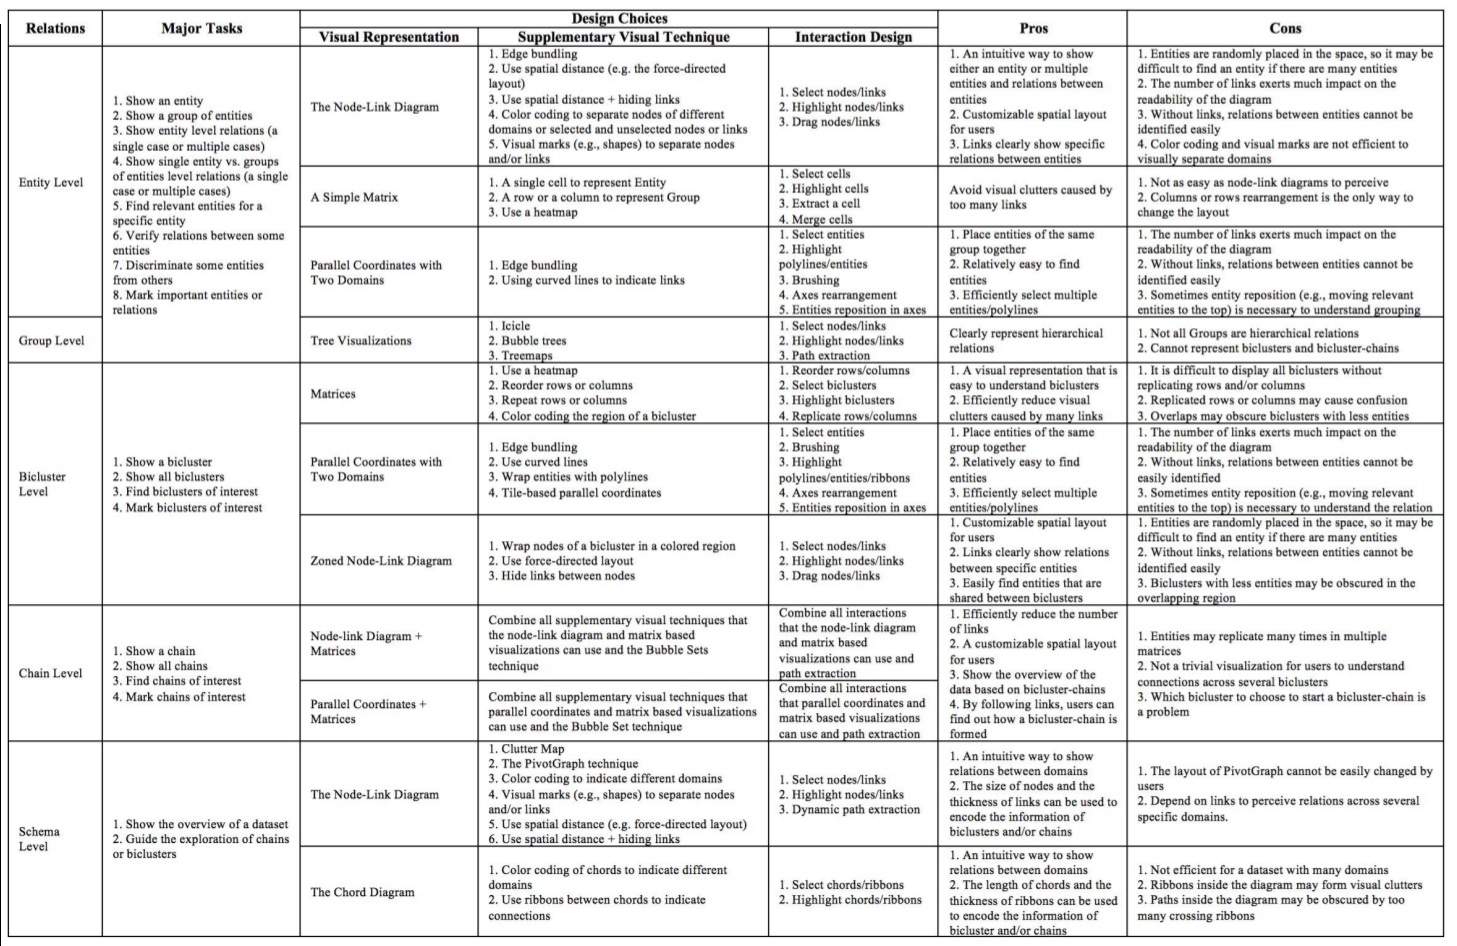
\includegraphics[width=1\textwidth]{images/sun2014five.png}
\caption{Design framework associated with bicluster visualization. Courtesy of Sun et al.\ \cite{sun2014five}.} \label{fig: sun2014five}
\end{center}
\end{figure}

%\item \textit{Classification Dimensions:}
%\begin{itemize}
%\item[~]\begin{center} Classifcation Structure: 2D Hierarchical \end{center}
%\item[X:] Major Tasks, Design Choices, Pros, Cons.
%\item[Y:] Relations: [Entity Level, Group Level, BiCluster Level, Chain Level, Schema Level]
%\item \textbf{Site:} n/a \url{}
%\item \textbf{Papers:} 93 Papers cited in Survey \{1972-2014\}\\
%\end{itemize}


%\item \textit{Unsolved Problems/Future Research:}
They identify three challenges in the field. The first challenge is the creation of an example  that implements design options across all five levels of the framework. The second challenge discusses traversal between the different levels. The final challenge suggests optimal layout of bi-cluster chains in visualization.

%\end{enumerate}

%Title: \textit{Formalizing Emphasis in Information Visualization} by Hall et al.\ \cite{hall2016formalizing}
%\begin{enumerate}
%\item \textit{The Concept:}
Hall et al.\ present a mathematical Framework for Information Visualization Emphasis (FIVE) by reviewing existing emphasis literature and frameworks \cite{hall2016formalizing}. Some examples of emphasis provided include highlighting regions of interest, animating data points, and altering the size of data points.
%\item \textit{The Scope:}
They first present a language for emphasizing sub-sets of data, and present a table displaying how their framework compares to previous solutions (see Figure \ref{fig: hall2016formalizing}). The paper then discusses different types of emphasis effects and how they can be used such as position, color, motion and transparency. Finally, the paper discusses the opportunities to use FIVE and some future directions for research.

%\item \textit{Classification:}
The frameworks are split into three categories. (1) \textit{Magnification} - papers that describe magnification emphasis effects. (2) \textit{Beyond magnification} - papers describing non-magnification emphasis effects. (3) \textit{Data suppression} - papers that focus on the creation of emphasis effects through data suppression. 

\begin{figure}[p]
\begin{center}
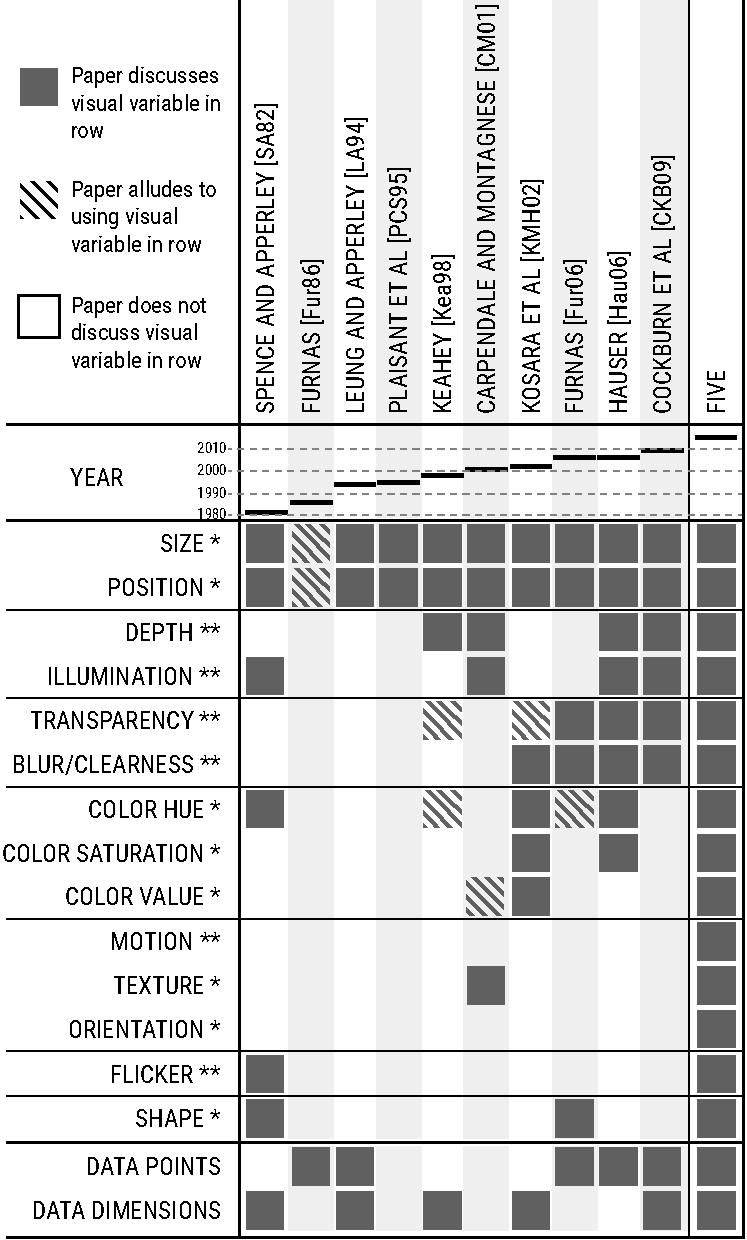
\includegraphics[width=0.8\textwidth]{images/hall2016formalizingFull}
\caption{Hall et al.\ present a table used to classify previous emphasis frameworks to diagnose what types of emphasis are discussed, and compare them to FIVE \cite{hall2016formalizing}  .} \label{fig: hall2016formalizing}
\end{center}
\end{figure}

%\item \textit{Classification Dimensions:}
%\begin{itemize}
%\item[~]\begin{center} Classification Structure: 4D \end{center}
%%\item[List:]
%\item[X:] Frameworks
%\item[Y:] Year, Size, Position, Depth, Illumination, Transparency, Blur/Clearness, Color Hue, Color Saturation, Color Value, Motion, Texture, Orientation, Flicker, Shape, Data Points, Data Dimensions.
%\item[Z$^1$:] Texture: [Variable discussed, Variable alluded, Variable not discussed]
%\item[Z$^2$:] $*$ - early visual variables,\\ $**$ - recent visual variables
%
%\item \textbf{Site:} n/a \url{}
%\item \textbf{Papers:} 81 Papers cited in Survey \{1982-2016\}\\
%\end{itemize}

%\item \textit{Unsolved Problems/Future Research:}
They provide four areas for future work: creating emphasis effects using under-explored visual variables and time variation, exploring alternative ways to vary data point prominence to create emphasis effects, providing a richer space of how to define and implement emphasis effects, and conducting empirical studies of emphasis effects.

%\end{enumerate}

\subsection{Overview Surveys}
Surveys that attempt to cover information visualization as a whole are presented here. This section summarizes two papers that review recent advancements in information visualization.

We summarize one survey that reviews the use of interactive lenses in visualization.
%Title: \textit{A Survey on Interactive Lenses in Visualization} by Tominski et al. \cite{tominski2014survey}
%\begin{enumerate}
%\item \textit{The Concept:}
Tominski et al.\ aim to analyze the use of interactive lenses in the context of visualization by reviewing the different techniques used to create lenses, whilst also helping researchers identify when to use interactive lenses. They discuss applicable data types such as geo-spatial data, why incorporating lenses is beneficial to the user experience, and some important techniques to be aware of if you are interested in this type of visualization. An interactive lens is defined as \textit{`to provide an on
demand alternative visual representation of the data underlying a local area of the screen'} \cite{tominski2014survey}.
%\item \textit{The Scope:}
After introducing the model of the interactive lens as well as the discussion of lens usage, they segment the research into interaction types. This includes examination of mouse and keyboard interaction, touch and multi-touch interaction, tangible interaction, tangible views and spatial interaction, gaze-based interaction and head tracking. \cite{tominski2014survey}

%\item \textit{Classification: }
The taxonomy of Tominski et al's survey examines both the data types that each visualization technique demonstrates (temporal, geospatial, flow, etc.), as well as the task that is achieved using it (across a total of 43 papers). This taxonomy enables discussion of possible future work such as the use of lenses for multi-user work (see Figure \ref{fig: tominski2014survey}).

\begin{figure}[p]
\begin{center}
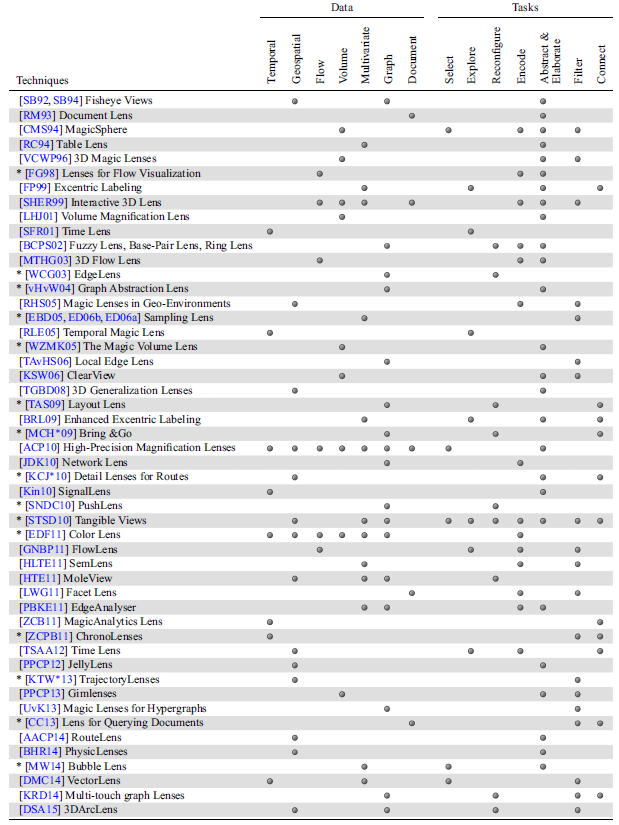
\includegraphics[width=0.85\textwidth]{images/tominski2014surveyFull}
\caption{Lens Techniques categorised according to data types and task. Courtesy of Tominski et al.\ \cite{tominski2016interactive}}\label{fig: tominski2014survey}
\end{center}
\end{figure}\vspace{-0.2cm}

%\item \textit{Classification Dimensions: }
%\begin{itemize}
%\item[X:]Data Type: [ Temporal, Geo-Spatial, Flow, Volume, Graph, Document],\\ Tasks: [Select, Explore, Reconfigure, Encode, Abstract \& Elaborate, Filter, Connect].
%\item[Y:] Magic Lens Techniques
%\item \textbf{Papers:} 43 Papers cited in Survey \{1983-2014\}
%\end{itemize}

%\item \textit{Unsolved Problems}
After reviewing some survey notes, they suggest that the need for more dynamic lenses with flexibility is an important design note as well as useful for a more varied use of functionality. Although mentioned in the survey, Tominski et al.\ would like to further investigate the development of multi-user or shared lenses, due to the growth in high-resolution and interactive displays. Finally, the idea of lens tool kits is an important focus area. Lenses are globally recognized visualization types but are in low use due to how interwoven they are with visualizations. With big data becoming a strong focus, this is something that needs further development. Tominski et al.\ also provide an extended version of the classification (see Figure \ref{fig: tominski2014survey}) \cite{tominski2016interactive}.

%\end{enumerate}
%Title: \textit{A Survey on Information Visualization - Recent Advances and Challenges} by Liu et al. \cite{liu2014survey}
%\begin{enumerate}
%\item \textit{The Concept:}
Liu et al.\ create a comprehensive study on the domain of information visualization. The aim of the paper is to derive an organization of the field, describing features, goals and state-of-the-art approaches for each category \cite{liu2014survey}.
%\item \textit{The Scope:}
The paper opens by examining the visualization pipeline and classification schemes. They proceed to present their 1-N taxonomy of the literature landscape within recent years, and present each topic whilst giving examples of papers in the related area. This continues on to communicating some technical challenges.

%\item \textit{Classification:}
Liu et al.\ break their taxonomy down into four main categories: empirical methodologies, interactions, frameworks, and applications. These categories are sub-divided into sub-categories (the figure is provided in the supplementary material). The classification has a lot of overlap with our organization. 


%\begin{figure}[ht]
%\begin{center}
%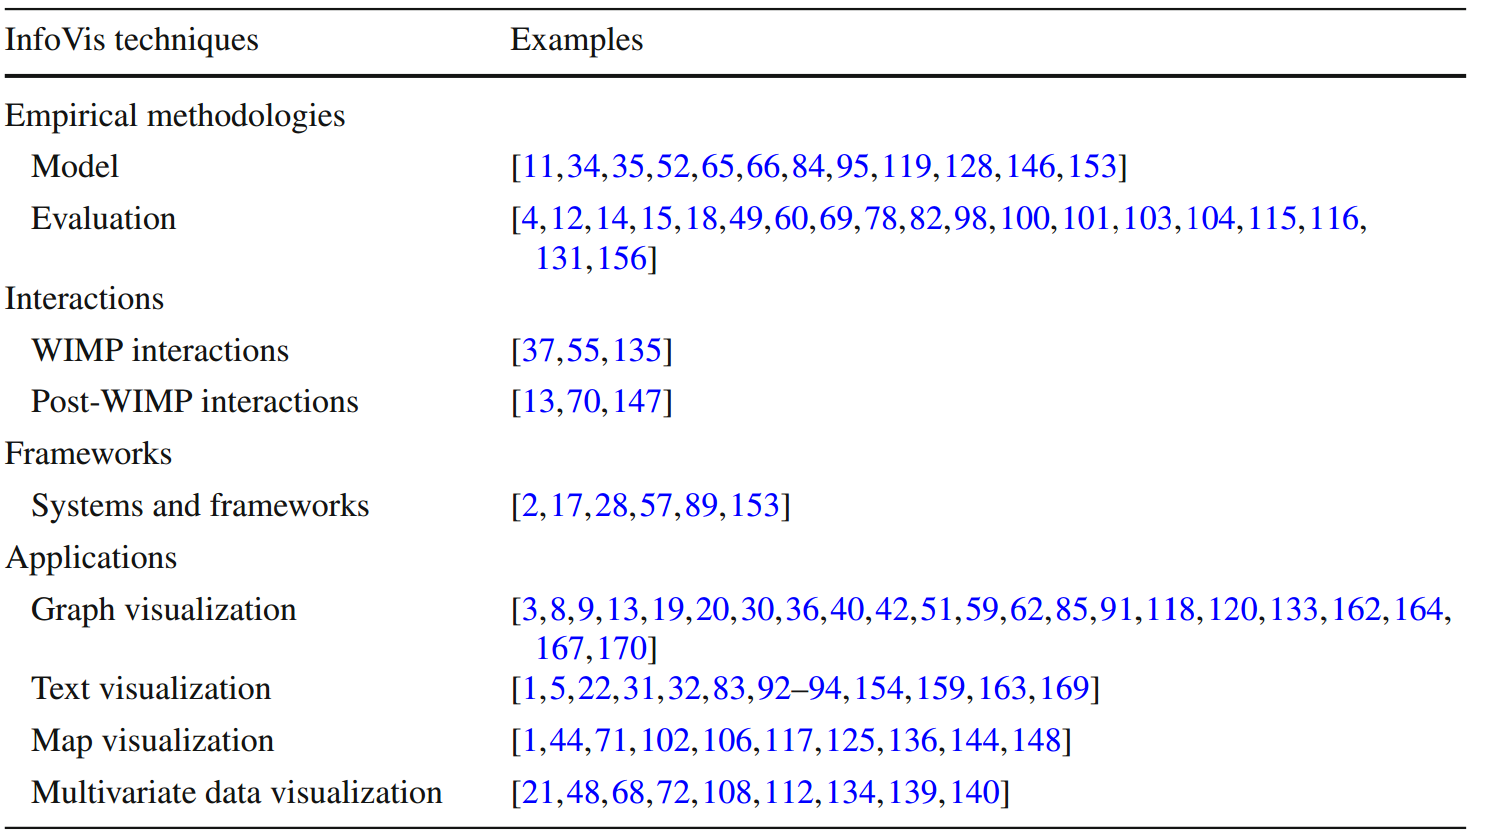
\includegraphics[width=0.5\textwidth]{images/liu2014survey.png}
%\caption{A taxonomy of InfoVis techniques created by Liu et al.\ \cite{liu2014survey}.} \label{fig: liu2014survey}
%\end{center}
%\end{figure}

%\item \textit{Classification Dimensions:}
%\begin{itemize}
%\item[~]\begin{center} Classifcation Structure: Hierarchical \end{center}
%\item[L:] Emperical Methods: [Model, Evaluation],\\
%Interactions: [WIMP interactions, Post-WIMP interactions],\\
%Frameworks: [Systems and Frameworks],\\
%Applications: [Graph Visualization, Map Visualization, Multivariate Data Visualization].
%\item \textbf{Site:} n/a \url{}
%\item \textbf{Papers:} 170 Papers cited in Survey \{1981-2012\}\\
%\end{itemize}

%\item \textit{Unsolved Problems/Future Research:}
Liu et al.\ describe an abundance of open research areas including usability, scalability, heterogeneous data, real-time visualization, and uncertainty.

%\end{enumerate}


%%%%%%%%%%%%%%%%%%%%%%%%%%%%%%%%
%%%CURRENT SURVEY SUMMARIES %%%%
%%%%%%%%%%%%%%%%%%%%%%%%%%%%%%%%






%%%%%%%%%%%%%%%%%%%%%%%%%%%%%%%%
%%%CURRENT SURVEY SUMMARIES %%%%
%%%%%%%%%%%%%%%%%%%%%%%%%%%%%%%%

\section{Future Work}
At the end of most survey papers, it is common for the authors to discuss future areas of work that are discovered over the course of the survey. These challenges and research directions have been compiled using SurVis, an online literature browser \cite{beck2016visual,surVis}. This enables us to find a number of future research areas within Information Visualization.

\begin{table}[p]
\scriptsize
\ra{1.15}
\centering


\begin{tabular}{|r|c|c|c|c|c|c|c|c|c|c|c|c|}

\rot{ \textbf{\textsc{Literature:}}}&\rot{\textsc{Evaluation}}&\rot{ \textsc{Missing Scenarios}}&\rot{ \textsc{Scalability}}&\rot{ \textsc{Interaction Techniques}}&\rot{ \textsc{Extended Data Dimensions}}&\rot{ \textsc{Tasks}~~~}&\rot{ \textsc{Tools}}&\rot{ \textsc{Fuzzyness \& Uncertainty}}&\rot{ \textsc{Time-Varying Data}}&\rot{ \textsc{Design Guidelines}}&\rot{ \textsc{heterogeneity}}\\ \hline
\fillCellSubHeader \cite{ahn2014task}					&&\fillItem &\fillItem &&&&&&\fillItem &&\\ \hline
\fillCellSubHeader \cite{alsallakh2014visualising}		&\fillItem &\fillItem &\fillItem &\fillItem &&&\fillItem &\fillItem &\fillItem &&\\ \hline
\fillCellSubHeader \cite{bach2014review}				&\fillItem &&&\fillItem &\fillItem &\fillItem &&&&&\\ \hline
\fillCellSubHeader \cite{beck2014state}				&\fillItem &\fillItem &\fillItem &\fillItem &\fillItem &&&&&&\\ \hline
\fillCellSubHeader \cite{behrisch2016matrix}			&\fillItem &&&&&&\fillItem &&&&\\ \hline
\fillCellSubHeader \cite{bertini2011quality}			&\fillItem &&\fillItem &&&&&&&&\\ \hline
\fillCellSubHeader \cite{borgo2013glyph}				&&&&&&&\fillItem &&&&\\ \hline
\fillCellSubHeader \cite{caserta2011visualization} 	&\fillItem &&&\fillItem &&&&&&&\\ \hline
\fillCellSubHeader \cite{chen2015survey}				&&&&&&&\fillItem &&&&\fillItem \\ \hline
\fillCellSubHeader \cite{cottam2012watch}				&\fillItem &\fillItem &&&&\fillItem &&&&&\\ \hline
\fillCellSubHeader \cite{elmqvist2010hierarchical}		&&&&&\fillItem &&&&&&\\ \hline
\fillCellSubHeader \cite{federico2016survey}			&\fillItem &\fillItem &\fillItem &\fillItem &&&&\fillItem &&&\\ \hline
\fillCellSubHeader \cite{fuchs2016systematic}			&\fillItem &\fillItem &&&&\fillItem &&&&&\\ \hline
\fillCellSubHeader \cite{gao2011performance}			&\fillItem &&\fillItem &&&&&&&&\\ \hline
\fillCellSubHeader \cite{hadlak2015survey}				&&\fillItem &&&&&&\fillItem &&&\fillItem\\ \hline
\fillCellSubHeader \cite{hall2016formalizing}			&\fillItem &\fillItem &&&&&&&&&\\ \hline
\fillCellSubHeader \cite{heinrich2013state}			&\fillItem &\fillItem &&&&\fillItem &&&&&\\ \hline
\fillCellSubHeader \cite{isaacs2014state}				&&\fillItem &\fillItem &&&&&&&&\\ \hline
\fillCellSubHeader \cite{janicke2015on}				&\fillItem &\fillItem &&&&&&\fillItem &&\fillItem &\\ \hline
\fillCellSubHeader \cite{javed2012exploring}			&&&&\fillItem &\fillItem &&&&\fillItem &&\\ \hline
\fillCellSubHeader \cite{johansson2016evaluation}		&&&&&\fillItem &&&&&&\\ \hline
\fillCellSubHeader \cite{kerracher2014design}			&&\fillItem &&&&&&&&&\\ \hline
\fillCellSubHeader \cite{kerracher2015task}			&&&&&&&\fillItem &&&&\\ \hline
\fillCellSubHeader \cite{kerracher2015visual}			&&\fillItem &&&&&&&&&\\ \hline
\fillCellSubHeader \cite{ko2016survey}					&\fillItem &\fillItem &&&&\fillItem &&&&&\\ \hline
\fillCellSubHeader \cite{kucher2015text}				&&&&&&&&&&&\\ \hline
\fillCellSubHeader \cite{liu2014survey}				&\fillItem &\fillItem &&&&\fillItem &&&&&\\ \hline
\fillCellSubHeader \cite{liu2015visualising}			&&&&\fillItem &&&&\fillItem &&&\\  \hline
\fillCellSubHeader \cite{nusrat2015task}				&&&&&&&&&&&\\ \hline
\fillCellSubHeader \cite{nusrat2016state}				&&\fillItem &\fillItem &&\fillItem &&&\fillItem &&&\\ \hline
\fillCellSubHeader \cite{schulz2011design}				&&&&&&&&&&\fillItem &\\ \hline
\fillCellSubHeader \cite{sedlmair2012taxonomy}			&&&&&&&&&&&\\ \hline
\fillCellSubHeader \cite{shiravi2012survey}			&&\fillItem &&\fillItem &&&&&&&\\ \hline
\fillCellSubHeader \cite{sun2014five}					&&&\fillItem &&&&\fillItem &&&\fillItem &\\ \hline
\fillCellSubHeader \cite{tominski2014survey}			&&&&\fillItem &&&\fillItem &&&&\\ \hline
\fillCellSubHeader \cite{vehlow2015state}				&\fillItem &&\fillItem &\fillItem &\fillItem &\fillItem &&&\fillItem &&\\ \hline
\fillCellSubHeader \cite{von2011visual}				&&&\fillItem &\fillItem &&\fillItem &&\fillItem &&&\\ \hline
\fillCellSubHeader \cite{wagner2015survey}				&&&\fillItem &\fillItem &\fillItem &&\fillItem &&&&\\ \hline
\fillCellSubHeader \cite{wanner2014state}				&\fillItem &\fillItem &\fillItem &&&&&&&&\\ \hline
\fillCellSubHeader \cite{zhou2015survey}				&\fillItem &&&&\fillItem &&&&&\fillItem &\\ 


%-------------------------------------------------------------------------------------------------------%
\hline
\end{tabular}
\caption{%$*$ Surveys not added are: \cite{blackwell1998taxonomy}.
The tables shows a breakdown of research directions discussed for each primary survey paper (highlighted \colorbox{lime}{green} in Table \ref{table: classificationTableClusters}). The directions displayed represent research areas that are discussed in more than one survey. This table corresponds to the 1-N classification example shown in Figure \ref{table:nMappingExamples} (B). }\label{table:futureWork}

\end{table}



The research topics found to have a high frequency (over 15\%) are listed in this section. Each topic provides a percentage of recently \textit{summarized} papers (40) that address a challenge found within the surveys.
\begin{enumerate}
\item \textbf{Evaluation (50\%):} The most frequent topic discussed for open-research directions is visualization evaluation. This includes user studies, qualitative studies, quantitative studies, and longitudinal studies. There is a strong focus on perceptual surveys, that would clearly show where studies are limited within each topic.
\item \textbf{Missing Scenarios (40\%):} Many topics point out vacant research scenarios within their classification tables. All of these topics are subject specific, and can be viewed using our literature browser \cite{surVis}.
\item \textbf{Scalability (35\%):} Scalability is still a very important trend in visualization design at the moment. This includes large datasets, the ability to move between views clearly, reducing clutter, and improving visual  understanding of complex views.
\item \textbf{Interaction Techniques (28\%):} The use of interaction techniques continues to be an essential part of visualization design in the recent decade. Research that discusses ways to filter or manipulate visualization seem to be an important topic in the upcoming future.
\item \textbf{Extended Data Dimensions (25\%):} Many surveys suggest that new data dimensions can be explored in the field. This differs from Item 2 by discussing the extension of a taxonomy.
\item \textbf{Tools (20\%):} A number of papers describe the need for new tools for their domain which includes a need for both generic tools or frameworks to enable users to quickly use techniques over multiple pieces of software, or context sensitive tools to allow specific test or an understanding within the field.
\item \textbf{Tasks (20\%):} 20\% of papers suggest that a stronger focus needs to be placed on exploring different tasks within each topic. This would enable researchers more understanding when a technique is appropriate, what approaches would produce the best output, and what can be gathered from visualization design choices.
\item \textbf{Fuzziness and Uncertainty (18\%):} Fuzziness and Uncertainty are a growing topic within Information Visualization and the results of our survey shows that this is a positive step. Visualization aims to represent clear findings and it is therefore essential that and uncertainty is represented. This open research topic was mainly suggested for text-focused surveys and multivariate surveys. Although there are uncertainty surveys published, only one of these fulfills one of our topics \cite{dasgupta2012conceptualizing}, while the other two are SciVis papers \cite{uncertain,brodlie2012}, so this research area is still open for research.
\end{enumerate}

Our paper presents some interesting findings. Graph surveys and text surveys have a large quantity of survey work in recent years. This enables quite a large overview of the current landscape of the topics but will also make it difficult to justify the creation of new surveys in the field. There is a large quantity of user studies across many fields yet there is little evidence of their use. Perceptual surveys are a great tool to analyze and document user-studies within a field, with the two papers summarized in this category giving a greater understanding of their benefit and contribution to the field \cite{johansson2016evaluation, fuchs2016systematic} (see Table \ref{table:futureWork} and figure \ref{fig: openresearch}). We also look how these papers are used in the field. We found that over 50\% of survey topics show a positive trend between surveys before and after 2010 (see Figure \ref{fig: cited}).


\begin{figure*}[t]
\begin{center}
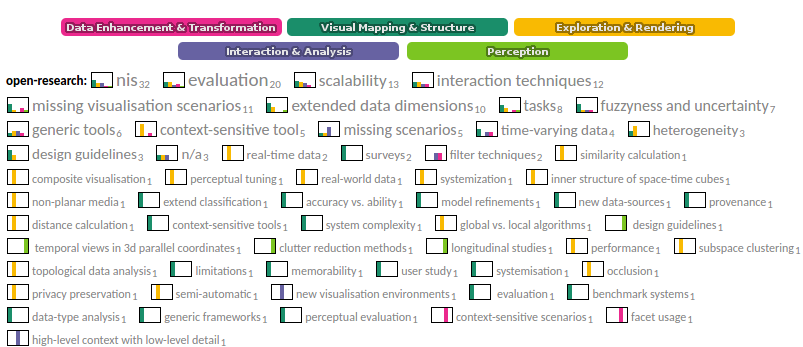
\includegraphics[width=0.98\textwidth]{images/open-research2.png}
\caption{Open research keywords collected across all recent, reviewed survey papers (2010-2017). \textit{`nis'} refers to papers not summarised. \textit{`n/a'} refers to summarised papers with no explicit open-research. Collected Keywords are reviewed using the SurVis Literature Browser \cite{beck2016visual, surVis}.} \label{fig: openresearch}
\end{center}
\end{figure*}

\section{Limitations}
There are some important considerations when looking at the implementation of the Survey of Surveys. The SoS uses natural topic clusters to classify literature in the field of information visualization. This means that topics reviewed are naturally biased towards surveys that have been published. A second limitation is that open-research is only based on what is discussed within each survey and this does not necessarily fully represent the current landscape of the domain, as there is a possibility that papers have been presented that fulfill open research directions between the publication of the survey and the publication of the SoS. This means that the older the paper, the more uncertain we are that the open research areas have matured.

\section{Conclusion}
The SoS contributes a quantum step forward in literature surveys. We present a novel classification of survey papers that enables the reader to find recently published literature among a wide variety of topics. The classification also enables users to easily spot areas of open-research for survey publication, as well as an understanding of broad open research topics in the field of information visualization. The paper provides a basic systematization of classification tables among the existing survey literature. It provides a valuable starting point for both newcomers and experienced researchers in visualization. We also believe it provides a valuable resource to readers outside of the information visualization and visual analytics communities. 

%\section{Acknowledgments}
%We would like to thank KESS for contributing funding towards this endeavor. Knowledge Economy Skills Scholarships (KESS) is a pan-Wales higher level skills initiative led by Bangor University on behalf of the HE sector in Wales. It is partially funded by the Welsh Government's European Social Fund (ESF) convergence programme for West Wales and the Valleys. We would also like to thank Richard Roberts, Dylan Rees, Thomas Basketter, and Dave Greten for help with proofreading the paper before submission. We also thank Wolfgang Aigner, Raimund Dachselt, Kyle Hall, Petra Isenberg, Johannes Kehrer, Catherine Plaisant, Alexander Rind, Ben Schneiderman, Christian Tominski, and Markus Wagner for providing feedback on the paper. We thank Helwig Hauser for the inspirational discussions on survey papers.

\begin{figure*}[t]
\begin{center}
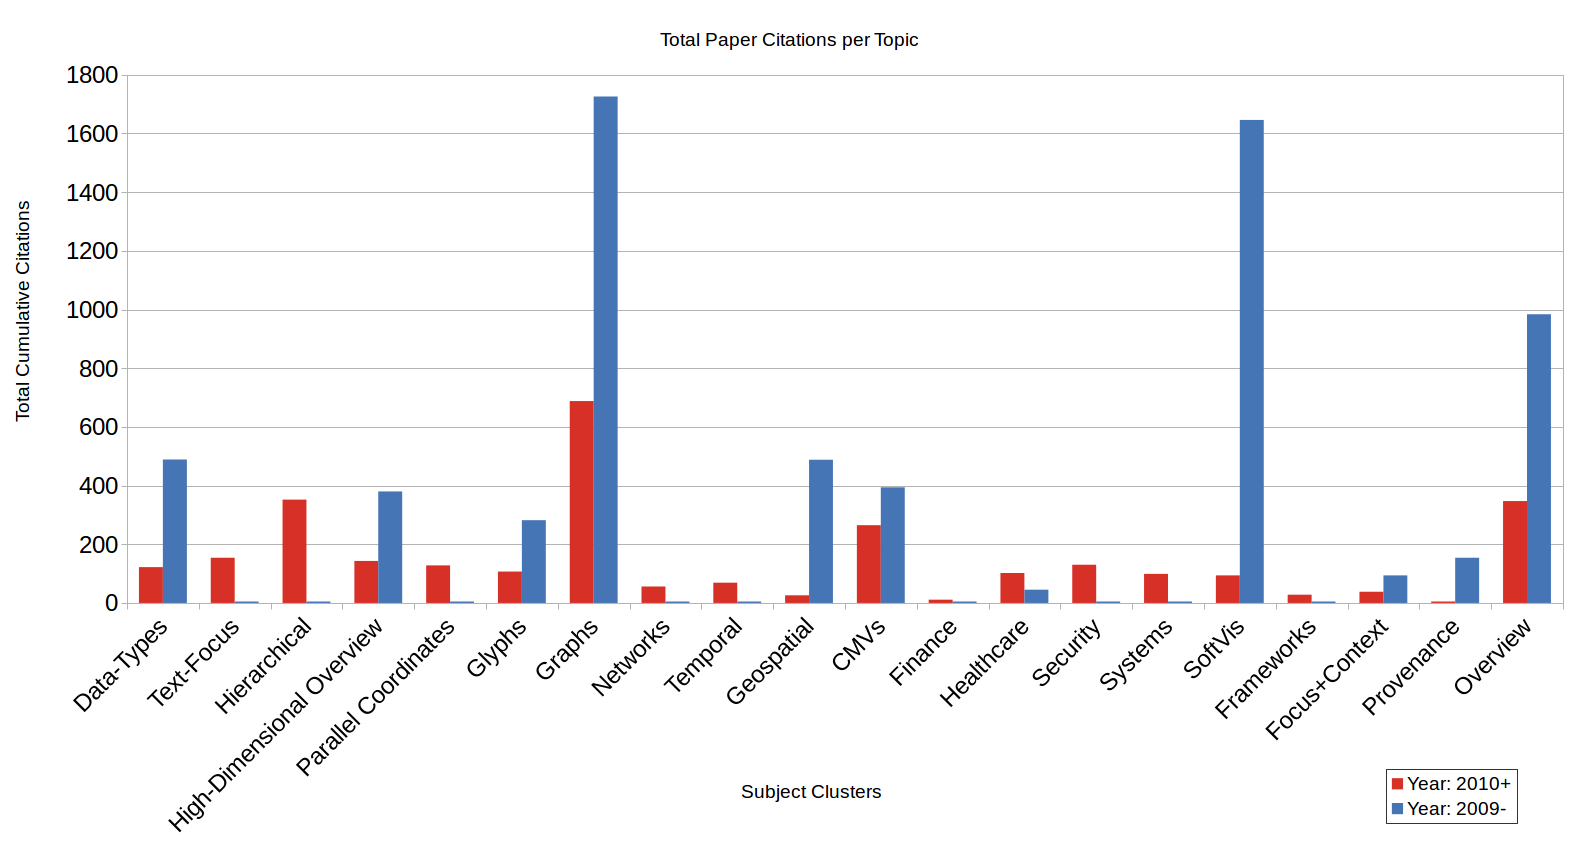
\includegraphics[width=1\textwidth]{images/CitedVis}
\caption{The graph provides a visualization of paper citations, ordered by topic, highlighting the difference between surveys published before and after 2010. The graph shows that 11 of the 20 show a positive trend, 10 of which are considered new subject clusters.} \label{fig: cited}
\end{center}
\end{figure*}